%%%%%%%%%%%%%%%%%%%%%%%%%%%%%%%%%%%%%%%%%%%%%%%%%%%%%%%%%%%%%%%%%%%%%%%%
% Uni Duesseldorf
% Lehrstuhl fuer Datenbanken und Informationssysteme
% Vorlage fuer Bachelor-/Masterarbeiten
% Optimiert fuer den Original-Latex-Kompiler LATEX.EXE (LaTeX=>PS=>PDF)
%%%%%%%%%%%%%%%%%%%%%%%%%%%%%%%%%%%%%%%%%%%%%%%%%%%%%%%%%%%%%%%%%%%%%%%%
% Ueberarbeitung f�r pdflatex (LaTeX=>PDF)
%%%%%%%%%%%%%%%%%%%%%%%%%%%%%%%%%%%%%%%%%%%%%%%%%%%%%%%%%%%%%%%%%%%%%%%%

% Die folgende Zeile NICHT EDITIEREN oder loeschen
%%%%%%%%%%%%%%%%%%%%%%%%%%%%%%%%%%%%%%%%%%%%%%%%%%%%%%%%%%%%%%%%%%%%%%%%
%%%% BEGINN EINSTELLUNG FUER DIE ARBEIT. UNBEDINGT ERFORDERLICH! %%%%%%%
%%%%%%%%%%%%%%%%%%%%%%%%%%%%%%%%%%%%%%%%%%%%%%%%%%%%%%%%%%%%%%%%%%%%%%%%
% Geben Sie Ihren Namen hier an:
\newcommand{\bearbeiter}{Michael Janschek}

% Geben Sie hier den Titel Ihrer Arbeit an:
\newcommand{\titel}{Classification of data\\ from the ATLAS experiments}

% Geben Sie das Datum des Beginns und Ende der Bachelorarbeit ein:
\newcommand{\beginndatum}{10. Dezember 2015}
\newcommand{\abgabedatum}{10.~März~2016}

% Geben Sie die Namen des Erst- und Zweitgutachters an:
\newcommand{\erstgutachter}{Prof. Dr. Stefan Harmeling}
\newcommand{\zweitgutachter}{Prof. Dr. Stefan Conrad}

% Falls Sie die Arbeit zweiseitig ausdrucken wollen,
% benutzen Sie die folgende Zeile mit
% \AN fuer zweiseitigen Druck
% \AUS fuer einseitigen Druck
\newcommand{\zweiseitig}{\AN}

% Falls die Arbeit in englischer Sprache verfasst 
% werden soll, dann benutzen Sie die folgende Zeile mit
% englisch fuer englische Sprache
% deutsch fuer deutsche Sprache
\newcommand{\sprache}{englisch}

% Hier wird eingestellt, ob es sich bei der Arbeit um eine Bachelor- 
% oder Masterarbeit handelt (unpassendes auskommentieren!):
\newcommand{\arbeit}{Bachelor Thesis}
%~ \newcommand{\arbeit}{Masterarbeit}
%%%%%%%%%%%%%%%%%%%%%%%%%%%%%%%%%%%%%%%%%%%%%%%%%%%%%%%%%%%%%%%%%%%%%%%%
%%%% ENDE EINSTELLUNGEN %%%%%%%%%%%%%%%%%%%%%%%%%%%%%%%%%%%%%%%%%%%%%%%%
%%%%%%%%%%%%%%%%%%%%%%%%%%%%%%%%%%%%%%%%%%%%%%%%%%%%%%%%%%%%%%%%%%%%%%%%

%%%%%%%%%%%%%%%%%%%%%%%%%%%%%%%%%%%%%%%%%%%%%%%%%%%%%%%%%%%
% Obere Titelmakros. Editieren Sie diese Datei nur, wenn
% Sie sich ABSOLUT sicher sind, was Sie da tun!!!
% (Z.B. zum Abaendern der BA-Vorlage in eine MA-Vorlage)
% Uni Duesseldorf
% Lehrstuhl fuer Datenbanken und Informationssysteme
% Version 2.2 - 2.3.2010
%%%%%%%%%%%%%%%%%%%%%%%%%%%%%%%%%%%%%%%%%%%%%%%%%%%%%%%%%%%
\newcommand{\AN}{twoside}
\newcommand{\AUS}{}
\newcommand{\englisch}{}
%\newcommand{\deutsch}{\usepackage[german]{babel}}

%% Die folgenden auskommentierten Optionen dienen der automatischen
%% Erkennung des Latex-Kompilers und dem Setzen der davon abhängigen
%% Einstellungen. Bei Problem z.B. mit dem Einbinden von verschiedenen
%% Grafiktypen bei Verwendung von PdfLatex oder Latex, einfach die
%% verschiedenen \usepackage(s) ausprobieren. (Mit diesen Einstellungen
%% funktionierte diese Vorlage bei der Verwenundg von latex.exe als
%% Kompiler bei den meisten Studierenden.)

%\newif\ifpdf \ifx\pdfoutput\undefined
%\pdffalse % we are not running pdflatex
%\else
%\pdfoutput=1 % we are running pdflatex
%\pdfcompresslevel=9 % compression level for text and image;
%\pdftrue \fi



\documentclass[11pt,a4paper, \zweiseitig]{article}

%used packages
%%%%%%%%%%%%%%%%%%%%%%%%%%notebook-packages%%%%%%%%%%%%%%%%%%%%%%%%%%%%%%%%%%%%%	
	\usepackage{graphicx} % Used to insert images
    %\usepackage{adjustbox} % Used to constrain images to a maximum size 
    %\usepackage{color} % Allow colors to be defined
    \usepackage[svgnames]{xcolor}
    \usepackage{listings}
    \usepackage{enumerate} % Needed for markdown enumerations to work
    \usepackage{amsmath} % Equations
    \usepackage{amssymb} % Equations
    \usepackage{eurosym} % defines \euro
    \usepackage[mathletters]{ucs} % Extended unicode (utf-8) support
    %\usepackage[utf8x]{inputenc} % Allow utf-8 characters in the tex document
    
%%%%%%%%%FOLLOWING HAS TO BE IN THIS VERY ORDER!!!%%%%%%%%%%
    \usepackage{fancybox,fancyvrb} % verbatim replacement that allows latex

    \usepackage{grffile} % extends the file name processing of package graphics 
                         % to support a larger range 
    % The hyperref package gives us a pdf with properly built
    % internal navigation ('pdf bookmarks' for the table of contents,
    % internal cross-reference links, web links for URLs, etc.)
    \usepackage{hyperref}
    \usepackage{longtable} % longtable support required by pandoc >1.10
    \usepackage{booktabs}  % table support for pandoc > 1.12.2
    
    \usepackage{tikz} % Needed to box output/input
    \usepackage{scrextend} % Used to indent output
    \usepackage{needspace} % Make prompts follow contents
    \usepackage{framed} % Used to draw output that spans multiple pages
%%%%%%%%%%%%%%%%%%%%%%%%%%notebook-packages%%%%%%%%%%%%%%%%%%%%%%%%%%%%%%%%%%%%%	

	\usepackage[inner=4cm,outer=2cm]{geometry} % Used to adjust the document margins
    
    \usepackage{ifthen} % ithenelse-command
    \usepackage{color} % allow color-definitions
    \usepackage{fancyhdr}

	%\usepackage[iso]{umlaute}
	\usepackage[utf8x]{inputenc}
	%\usepackage{makeidx} % um ein Index zu erstellen
	
	
%%%%%%%%%%%%%%%%%%%%%%%%%%%%%%%%%%%%% Font %%%%%%%%%%%%%%%%%%%%%%%%%%%%%%%%%%%%%
	
	\usepackage[nottoc]{tocbibind}
	\usepackage[T1]{fontenc} %fuer richtige Trennung bei Umlauten
	\usepackage{lmodern}            % have lmtt loaded; but...
	\usepackage{palatino} % palatino Schriftart, %%nicht kompatibel mit Jupyter
	%\usepackage{tgpagella}          % use "palatino" as main font, ...
	\renewcommand{\ttdefault}{lmtt} % and use lmtt for teletype family
%%%%%%%%%%%%%%%%%%%%%%%%%%%%%%%%%%%%%%%%%%%%%%%%%%%%%%%%%%%%%%%%%%%%%%%%%%%%%%%%	
	\usepackage{shortvrb}

	\usepackage{a4wide} % ganze A4 Weite verwenden
	
	%\usepackage{babelbib} %BibTex auf englisch
	%\selectbiblanguage{english}

%%%%%%%%%%%%% USER-PACKAGES %%%%%%%%%%%%%%%%
	\usepackage{caption}
	\usepackage{subcaption}
	
	
	%\ifpdf
	%\usepackage[pdftex,xdvi]{graphicx}
	%\usepackage{thumbpdf} %thumbs fuer Pdf
	%\usepackage[pdfstartview=FitV]{hyperref} %anklickbares Inhaltsverzeichnis
	%\else
	%\usepackage[dvips,xdvi]{graphicx}
	%\usepackage{graphicx}
	%\usepackage{hyperref} %anklickbares Inhaltsverzeichnis
	%\fi

%%%%%%%%%%%%%%%%%%%%%%%%%%%%%%% fancy Headline %%%%%%%%%%%%%%%%%%%%%%%%%%%%%%%%%

\fancyhf{}
\pagestyle{fancy}
\definecolor{bleudefrance}{rgb}{0.0745, 0.4431, 0.7843} %HHU-Blau
\renewcommand{\headrule}
	{{\color{bleudefrance}%
		\hrule height 2pt
			width\headwidth
		\vspace{1pt}%
		\hrule height 1pt
			width\headwidth
		\vspace{-4pt}
	}
	{\renewcommand{\headrulewidth}{15cm} % remove lines as well
	}}
\renewcommand{\sectionmark}[1]{ \markboth{#1}{} }

\ifthenelse{\equal{\zweiseitig}{twoside}}
	{\fancyhead[LE]{\thepage \hskip6mm \textit{\nouppercase{\leftmark}}}}
	{\fancyhead[LO]{\textit{\nouppercase{\leftmark}}}}
\fancyhead[RO]{\textit{\nouppercase{\rightmark} \hskip6mm \thepage}}

%%%%%%%%%%%%%%%%%%%%%%% Massangaben fuer die Arbeit %%%%%%%%%%%%%%%

\setlength{\textwidth}{15cm}

\setlength{\oddsidemargin}{40mm}
\setlength{\evensidemargin}{20mm}

\addtolength{\oddsidemargin}{-1in}
\addtolength{\evensidemargin}{-1in}

%\makeindex
\hypersetup{
      breaklinks=true,  % so long urls are correctly broken across lines
      colorlinks=true,
      urlcolor=blue,
      linkcolor=darkorange,
      citecolor=darkgreen,
      }
%set notebook configs
\definecolor{orange}{cmyk}{0,0.4,0.8,0.2}
    \definecolor{darkorange}{rgb}{.71,0.21,0.01}
    \definecolor{darkgreen}{rgb}{.12,.54,.11}
    \definecolor{myteal}{rgb}{.26, .44, .56}
    \definecolor{gray}{gray}{0.45}
    \definecolor{lightgray}{gray}{.95}
    \definecolor{mediumgray}{gray}{.8}
    \definecolor{inputbackground}{rgb}{.95, .95, .85}
    \definecolor{outputbackground}{rgb}{.95, .95, .95}
    \definecolor{traceback}{rgb}{1, .95, .95}
    % ansi colors
    \definecolor{red}{rgb}{.6,0,0}
    \definecolor{green}{rgb}{0,.65,0}
    \definecolor{brown}{rgb}{0.6,0.6,0}
    \definecolor{blue}{rgb}{0,.145,.698}
    \definecolor{purple}{rgb}{.698,.145,.698}
    \definecolor{cyan}{rgb}{0,.698,.698}
    \definecolor{lightgray}{gray}{0.5}
    
    % bright ansi colors
    \definecolor{darkgray}{gray}{0.25}
    \definecolor{lightred}{rgb}{1.0,0.39,0.28}
    \definecolor{lightgreen}{rgb}{0.48,0.99,0.0}
    \definecolor{lightblue}{rgb}{0.53,0.81,0.92}
    \definecolor{lightpurple}{rgb}{0.87,0.63,0.87}
    \definecolor{lightcyan}{rgb}{0.5,1.0,0.83}
    
    % Exact colors from NB
    \definecolor{incolor}{rgb}{0.0, 0.0, 0.5}
    \definecolor{outcolor}{rgb}{0.545, 0.0, 0.0}
    
    % commands and environments needed by pandoc snippets
    % extracted from the output of `pandoc -s`
    \providecommand{\tightlist}{%
      \setlength{\itemsep}{0pt}\setlength{\parskip}{0pt}}
      
	\definecolor{shadecolor}{rgb}{.9, .9, .9}
    %\DefineVerbatimEnvironment{Highlighting}{Verbatim}{
    
%%%%%%%%%%%%%%magic%%%%%%%%%%%%%%

	\RecustomVerbatimEnvironment{Verbatim}{Verbatim}{
		commandchars=\\\{\},
		fontsize=\small,
		frame=leftline,
		rulecolor=\color{gray},
	}
    
    \DefineVerbatimEnvironment{Highlighting}{Verbatim}{
    	commandchars=\\\{\},
    	%bgcolor=shadecolor,
%	   	fontfamily=courier,
    	fontsize=\small,
%		gobble=2,
%		numbers=left,
%		numbersep=2mm,
		}
    % Add ',fontsize=\small' for more characters per line
    \newenvironment{Shaded}{}{}
    \newcommand{\KeywordTok}[1]{\textcolor[rgb]{0.00,0.44,0.13}{\textbf{{#1}}}}
    \newcommand{\DataTypeTok}[1]{\textcolor[rgb]{0.56,0.13,0.00}{{#1}}}
    \newcommand{\DecValTok}[1]{\textcolor[rgb]{0.25,0.63,0.44}{{#1}}}
    \newcommand{\BaseNTok}[1]{\textcolor[rgb]{0.25,0.63,0.44}{{#1}}}
    \newcommand{\FloatTok}[1]{\textcolor[rgb]{0.25,0.63,0.44}{{#1}}}
    \newcommand{\CharTok}[1]{\textcolor[rgb]{0.25,0.44,0.63}{{#1}}}
    \newcommand{\StringTok}[1]{\textcolor[rgb]{0.25,0.44,0.63}{{#1}}}
    \newcommand{\CommentTok}[1]{\textcolor[rgb]{0.38,0.63,0.69}{\textit{{#1}}}}
    \newcommand{\OtherTok}[1]{\textcolor[rgb]{0.00,0.44,0.13}{{#1}}}
    \newcommand{\AlertTok}[1]{\textcolor[rgb]{1.00,0.00,0.00}{\textbf{{#1}}}}
    \newcommand{\FunctionTok}[1]{\textcolor[rgb]{0.02,0.16,0.49}{{#1}}}
    \newcommand{\RegionMarkerTok}[1]{{#1}}
    \newcommand{\ErrorTok}[1]{\textcolor[rgb]{1.00,0.00,0.00}{\textbf{{#1}}}}
    \newcommand{\NormalTok}[1]{{#1}}
    
    % Define a nice break command that doesn't care if a line doesn't already
    % exist.
    \def\br{\hspace*{\fill} \\* }
    % Math Jax compatability definitions
    \def\gt{>}
    \def\lt{<}
    
    % Pygments definitions
    
\makeatletter
\def\PY@reset{\let\PY@it=\relax \let\PY@bf=\relax%
    \let\PY@ul=\relax \let\PY@tc=\relax%
    \let\PY@bc=\relax \let\PY@ff=\relax}
\def\PY@tok#1{\csname PY@tok@#1\endcsname}
\def\PY@toks#1+{\ifx\relax#1\empty\else%
    \PY@tok{#1}\expandafter\PY@toks\fi}
\def\PY@do#1{\PY@bc{\PY@tc{\PY@ul{%
    \PY@it{\PY@bf{\PY@ff{#1}}}}}}}
\def\PY#1#2{\PY@reset\PY@toks#1+\relax+\PY@do{#2}}

\expandafter\def\csname PY@tok@nc\endcsname{\let\PY@bf=\textbf\def\PY@tc##1{\textcolor[rgb]{0.00,0.00,1.00}{##1}}}
\expandafter\def\csname PY@tok@se\endcsname{\let\PY@bf=\textbf\def\PY@tc##1{\textcolor[rgb]{0.73,0.40,0.13}{##1}}}
\expandafter\def\csname PY@tok@gt\endcsname{\def\PY@tc##1{\textcolor[rgb]{0.00,0.27,0.87}{##1}}}
\expandafter\def\csname PY@tok@ne\endcsname{\let\PY@bf=\textbf\def\PY@tc##1{\textcolor[rgb]{0.82,0.25,0.23}{##1}}}
\expandafter\def\csname PY@tok@gh\endcsname{\let\PY@bf=\textbf\def\PY@tc##1{\textcolor[rgb]{0.00,0.00,0.50}{##1}}}
\expandafter\def\csname PY@tok@kn\endcsname{\let\PY@bf=\textbf\def\PY@tc##1{\textcolor[rgb]{0.00,0.50,0.00}{##1}}}
\expandafter\def\csname PY@tok@nt\endcsname{\let\PY@bf=\textbf\def\PY@tc##1{\textcolor[rgb]{0.00,0.50,0.00}{##1}}}
\expandafter\def\csname PY@tok@nd\endcsname{\def\PY@tc##1{\textcolor[rgb]{0.67,0.13,1.00}{##1}}}
\expandafter\def\csname PY@tok@kp\endcsname{\def\PY@tc##1{\textcolor[rgb]{0.00,0.50,0.00}{##1}}}
\expandafter\def\csname PY@tok@il\endcsname{\def\PY@tc##1{\textcolor[rgb]{0.40,0.40,0.40}{##1}}}
\expandafter\def\csname PY@tok@gi\endcsname{\def\PY@tc##1{\textcolor[rgb]{0.00,0.63,0.00}{##1}}}
\expandafter\def\csname PY@tok@ss\endcsname{\def\PY@tc##1{\textcolor[rgb]{0.10,0.09,0.49}{##1}}}
\expandafter\def\csname PY@tok@kr\endcsname{\let\PY@bf=\textbf\def\PY@tc##1{\textcolor[rgb]{0.00,0.50,0.00}{##1}}}
\expandafter\def\csname PY@tok@gd\endcsname{\def\PY@tc##1{\textcolor[rgb]{0.63,0.00,0.00}{##1}}}
\expandafter\def\csname PY@tok@mb\endcsname{\def\PY@tc##1{\textcolor[rgb]{0.40,0.40,0.40}{##1}}}
\expandafter\def\csname PY@tok@sh\endcsname{\def\PY@tc##1{\textcolor[rgb]{0.73,0.13,0.13}{##1}}}
\expandafter\def\csname PY@tok@c1\endcsname{\let\PY@it=\textit\def\PY@tc##1{\textcolor[rgb]{0.25,0.50,0.50}{##1}}}
\expandafter\def\csname PY@tok@o\endcsname{\def\PY@tc##1{\textcolor[rgb]{0.40,0.40,0.40}{##1}}}
\expandafter\def\csname PY@tok@vc\endcsname{\def\PY@tc##1{\textcolor[rgb]{0.10,0.09,0.49}{##1}}}
\expandafter\def\csname PY@tok@gu\endcsname{\let\PY@bf=\textbf\def\PY@tc##1{\textcolor[rgb]{0.50,0.00,0.50}{##1}}}
\expandafter\def\csname PY@tok@m\endcsname{\def\PY@tc##1{\textcolor[rgb]{0.40,0.40,0.40}{##1}}}
\expandafter\def\csname PY@tok@sc\endcsname{\def\PY@tc##1{\textcolor[rgb]{0.73,0.13,0.13}{##1}}}
\expandafter\def\csname PY@tok@sb\endcsname{\def\PY@tc##1{\textcolor[rgb]{0.73,0.13,0.13}{##1}}}
\expandafter\def\csname PY@tok@w\endcsname{\def\PY@tc##1{\textcolor[rgb]{0.73,0.73,0.73}{##1}}}
\expandafter\def\csname PY@tok@go\endcsname{\def\PY@tc##1{\textcolor[rgb]{0.53,0.53,0.53}{##1}}}
\expandafter\def\csname PY@tok@gr\endcsname{\def\PY@tc##1{\textcolor[rgb]{1.00,0.00,0.00}{##1}}}
\expandafter\def\csname PY@tok@ow\endcsname{\let\PY@bf=\textbf\def\PY@tc##1{\textcolor[rgb]{0.67,0.13,1.00}{##1}}}
\expandafter\def\csname PY@tok@kd\endcsname{\let\PY@bf=\textbf\def\PY@tc##1{\textcolor[rgb]{0.00,0.50,0.00}{##1}}}
\expandafter\def\csname PY@tok@gp\endcsname{\let\PY@bf=\textbf\def\PY@tc##1{\textcolor[rgb]{0.00,0.00,0.50}{##1}}}
\expandafter\def\csname PY@tok@mi\endcsname{\def\PY@tc##1{\textcolor[rgb]{0.40,0.40,0.40}{##1}}}
\expandafter\def\csname PY@tok@c\endcsname{\let\PY@it=\textit\def\PY@tc##1{\textcolor[rgb]{0.25,0.50,0.50}{##1}}}
\expandafter\def\csname PY@tok@nb\endcsname{\def\PY@tc##1{\textcolor[rgb]{0.00,0.50,0.00}{##1}}}
\expandafter\def\csname PY@tok@vi\endcsname{\def\PY@tc##1{\textcolor[rgb]{0.10,0.09,0.49}{##1}}}
\expandafter\def\csname PY@tok@k\endcsname{\let\PY@bf=\textbf\def\PY@tc##1{\textcolor[rgb]{0.00,0.50,0.00}{##1}}}
\expandafter\def\csname PY@tok@ni\endcsname{\let\PY@bf=\textbf\def\PY@tc##1{\textcolor[rgb]{0.60,0.60,0.60}{##1}}}
\expandafter\def\csname PY@tok@no\endcsname{\def\PY@tc##1{\textcolor[rgb]{0.53,0.00,0.00}{##1}}}
\expandafter\def\csname PY@tok@cm\endcsname{\let\PY@it=\textit\def\PY@tc##1{\textcolor[rgb]{0.25,0.50,0.50}{##1}}}
\expandafter\def\csname PY@tok@nf\endcsname{\def\PY@tc##1{\textcolor[rgb]{0.00,0.00,1.00}{##1}}}
\expandafter\def\csname PY@tok@cs\endcsname{\let\PY@it=\textit\def\PY@tc##1{\textcolor[rgb]{0.25,0.50,0.50}{##1}}}
\expandafter\def\csname PY@tok@mo\endcsname{\def\PY@tc##1{\textcolor[rgb]{0.40,0.40,0.40}{##1}}}
\expandafter\def\csname PY@tok@err\endcsname{\def\PY@bc##1{\setlength{\fboxsep}{0pt}\fcolorbox[rgb]{1.00,0.00,0.00}{1,1,1}{\strut ##1}}}
\expandafter\def\csname PY@tok@kc\endcsname{\let\PY@bf=\textbf\def\PY@tc##1{\textcolor[rgb]{0.00,0.50,0.00}{##1}}}
\expandafter\def\csname PY@tok@s2\endcsname{\def\PY@tc##1{\textcolor[rgb]{0.73,0.13,0.13}{##1}}}
\expandafter\def\csname PY@tok@mf\endcsname{\def\PY@tc##1{\textcolor[rgb]{0.40,0.40,0.40}{##1}}}
\expandafter\def\csname PY@tok@bp\endcsname{\def\PY@tc##1{\textcolor[rgb]{0.00,0.50,0.00}{##1}}}
\expandafter\def\csname PY@tok@nl\endcsname{\def\PY@tc##1{\textcolor[rgb]{0.63,0.63,0.00}{##1}}}
\expandafter\def\csname PY@tok@cp\endcsname{\def\PY@tc##1{\textcolor[rgb]{0.74,0.48,0.00}{##1}}}
\expandafter\def\csname PY@tok@s\endcsname{\def\PY@tc##1{\textcolor[rgb]{0.73,0.13,0.13}{##1}}}
\expandafter\def\csname PY@tok@mh\endcsname{\def\PY@tc##1{\textcolor[rgb]{0.40,0.40,0.40}{##1}}}
\expandafter\def\csname PY@tok@vg\endcsname{\def\PY@tc##1{\textcolor[rgb]{0.10,0.09,0.49}{##1}}}
\expandafter\def\csname PY@tok@sr\endcsname{\def\PY@tc##1{\textcolor[rgb]{0.73,0.40,0.53}{##1}}}
\expandafter\def\csname PY@tok@gs\endcsname{\let\PY@bf=\textbf}
\expandafter\def\csname PY@tok@na\endcsname{\def\PY@tc##1{\textcolor[rgb]{0.49,0.56,0.16}{##1}}}
\expandafter\def\csname PY@tok@kt\endcsname{\def\PY@tc##1{\textcolor[rgb]{0.69,0.00,0.25}{##1}}}
\expandafter\def\csname PY@tok@s1\endcsname{\def\PY@tc##1{\textcolor[rgb]{0.73,0.13,0.13}{##1}}}
\expandafter\def\csname PY@tok@si\endcsname{\let\PY@bf=\textbf\def\PY@tc##1{\textcolor[rgb]{0.73,0.40,0.53}{##1}}}
\expandafter\def\csname PY@tok@ge\endcsname{\let\PY@it=\textit}
\expandafter\def\csname PY@tok@nn\endcsname{\let\PY@bf=\textbf\def\PY@tc##1{\textcolor[rgb]{0.00,0.00,1.00}{##1}}}
\expandafter\def\csname PY@tok@sd\endcsname{\let\PY@it=\textit\def\PY@tc##1{\textcolor[rgb]{0.73,0.13,0.13}{##1}}}
\expandafter\def\csname PY@tok@nv\endcsname{\def\PY@tc##1{\textcolor[rgb]{0.10,0.09,0.49}{##1}}}
\expandafter\def\csname PY@tok@sx\endcsname{\def\PY@tc##1{\textcolor[rgb]{0.00,0.50,0.00}{##1}}}

\def\PYZbs{\char`\\}
\def\PYZus{\char`\_}
\def\PYZob{\char`\{}
\def\PYZcb{\char`\}}
\def\PYZca{\char`\^}
\def\PYZam{\char`\&}
\def\PYZlt{\char`\<}
\def\PYZgt{\char`\>}
\def\PYZsh{\char`\#}
\def\PYZpc{\char`\%}
\def\PYZdl{\char`\$}
\def\PYZhy{\char`\-}
\def\PYZsq{\char`\'}
\def\PYZdq{\char`\"}
\def\PYZti{\char`\~}
% for compatibility with earlier versions
\def\PYZat{@}
\def\PYZlb{[}
\def\PYZrb{]}
\makeatother

 % NB prompt colors
    \definecolor{nbframe-border}{rgb}{0.867,0.867,0.867}
    \definecolor{nbframe-bg}{rgb}{0.969,0.969,0.969}
    \definecolor{nbframe-in-prompt}{rgb}{0.0,0.0,0.502}
    \definecolor{nbframe-out-prompt}{rgb}{0.545,0.0,0.0}

    % NB prompt lengths
    \newlength{\inputpadding}
    \setlength{\inputpadding}{0.5em}
    \newlength{\cellleftmargin}
    \setlength{\cellleftmargin}{0.15\linewidth}
    \newlength{\borderthickness}
    \setlength{\borderthickness}{0.4pt}
    \newlength{\smallerfontscale}
    \setlength{\smallerfontscale}{9.5pt}

    % NB prompt font size
    \def\smaller{\fontsize{\smallerfontscale}{\smallerfontscale}\selectfont}

    % Define a background layer, in which the nb prompt shape is drawn
    \pgfdeclarelayer{background}
    \pgfsetlayers{background,main}
    \usetikzlibrary{calc}

    % define styles for the normal border and the torn border
    \tikzset{
      normal border/.style={draw=nbframe-border, fill=nbframe-bg,
        rectangle, rounded corners=2.5pt, line width=\borderthickness},
      torn border/.style={draw=white, fill=white, line width=\borderthickness}}

    % Macro to draw the shape behind the text, when it fits completly in the
    % page
    \def\notebookcellframe#1{%
    \tikz{%
      \node[inner sep=\inputpadding] (A) {#1};% Draw the text of the node
      \begin{pgfonlayer}{background}% Draw the shape behind
      \fill[normal border]%
            (A.south east) -- ($(A.south west)+(\cellleftmargin,0)$) -- 
            ($(A.north west)+(\cellleftmargin,0)$) -- (A.north east) -- cycle;
      \end{pgfonlayer}}}%

    % Macro to draw the shape, when the text will continue in next page
    \def\notebookcellframetop#1{%
    \tikz{%
      \node[inner sep=\inputpadding] (A) {#1};    % Draw the text of the node
      \begin{pgfonlayer}{background}    
      \fill[normal border]              % Draw the ``complete shape'' behind
            (A.south east) -- ($(A.south west)+(\cellleftmargin,0)$) -- 
            ($(A.north west)+(\cellleftmargin,0)$) -- (A.north east) -- cycle;
      \fill[torn border]                % Add the torn lower border
            ($(A.south east)-(0,.1)$) -- ($(A.south west)+(\cellleftmargin,-.1)$) -- 
            ($(A.south west)+(\cellleftmargin,.1)$) -- ($(A.south east)+(0,.1)$) -- cycle;
      \end{pgfonlayer}}}

    % Macro to draw the shape, when the text continues from previous page
    \def\notebookcellframebottom#1{%
    \tikz{%
      \node[inner sep=\inputpadding] (A) {#1};   % Draw the text of the node
      \begin{pgfonlayer}{background}   
      \fill[normal border]             % Draw the ``complete shape'' behind
            (A.south east) -- ($(A.south west)+(\cellleftmargin,0)$) -- 
            ($(A.north west)+(\cellleftmargin,0)$) -- (A.north east) -- cycle;
      \fill[torn border]               % Add the torn upper border
            ($(A.north east)-(0,.1)$) -- ($(A.north west)+(\cellleftmargin,-.1)$) -- 
            ($(A.north west)+(\cellleftmargin,.1)$) -- ($(A.north east)+(0,.1)$) -- cycle;
      \end{pgfonlayer}}}

    % Macro to draw the shape, when both the text continues from previous page
    % and it will continue in next page
    \def\notebookcellframemiddle#1{%
    \tikz{%
      \node[inner sep=\inputpadding] (A) {#1};   % Draw the text of the node
      \begin{pgfonlayer}{background}   
      \fill[normal border]             % Draw the ``complete shape'' behind
            (A.south east) -- ($(A.south west)+(\cellleftmargin,0)$) -- 
            ($(A.north west)+(\cellleftmargin,0)$) -- (A.north east) -- cycle;
      \fill[torn border]               % Add the torn lower border
            ($(A.south east)-(0,.1)$) -- ($(A.south west)+(\cellleftmargin,-.1)$) -- 
            ($(A.south west)+(\cellleftmargin,.1)$) -- ($(A.south east)+(0,.1)$) -- cycle;
      \fill[torn border]               % Add the torn upper border
            ($(A.north east)-(0,.1)$) -- ($(A.north west)+(\cellleftmargin,-.1)$) -- 
            ($(A.north west)+(\cellleftmargin,.1)$) -- ($(A.north east)+(0,.1)$) -- cycle;
      \end{pgfonlayer}}}

    % Define the environment which puts the frame
    % In this case, the environment also accepts an argument with an optional
    % title (which defaults to ``Example'', which is typeset in a box overlaid
    % on the top border
    \newenvironment{notebookcell}[1][0]{%
      \def\FrameCommand{\notebookcellframe}%
      \def\FirstFrameCommand{\notebookcellframetop}%
      \def\LastFrameCommand{\notebookcellframebottom}%
      \def\MidFrameCommand{\notebookcellframemiddle}%
      \par\vspace{1\baselineskip}%
      \MakeFramed {\FrameRestore}%
      \noindent\tikz\node[inner sep=0em] at ($(A.north west)-(0,0)$) {%
    
      }; 
      \par}%
    {\endMakeFramed}

%%%%%%%%%%%%%%%%%%%%%%%%%%%%%%%%%%%%%%%%%%%%%%%%%%%%%%%%%%%%%%%%%%%%%%%%%%%%%%%%
\ifthenelse{\equal{\sprache}{deutsch}}{\usepackage[ngerman]{babel}}{}




\begin{document}

%\setcounter{secnumdepth}{4} %Nummerieren bis in die 4. Ebene
%\setcounter{tocdepth}{4} %Inhaltsverzeichnis bis zur 4. Ebene

%\pagestyle{headings}
%\pagestyle{fancy}

%%%%%%%%%%%%%%%%%%%%%%%%%%%%%%%%%%%%%%%%%%%%%%%%%%%%%%%%%%%%%%%%%%%%%%%%%%%%%%%%
\setlength{\headheight}{15pt}


%%%%%%%%%%%%%%%%%%%%%%%%%%%%%%%%%%%%%%%%%%%%%%%%%%%%%%%%%%%%%%%%%%%%%%%%%%%%%%%%


\sloppy % LaTeX ist dann nicht so streng mit der Silbentrennung
%~ \MakeShortVerb{\§}

\parindent0mm
\parskip0.5em


{
\textwidth170mm 
\oddsidemargin30mm 
\evensidemargin30mm 
\addtolength{\oddsidemargin}{-1in}
\addtolength{\evensidemargin}{-1in}

\parskip0pt plus2pt

% Die Raender muessen eventuell fuer jeden Drucker individuell eingestellt
% werden. Dazu sind die Werte fuer die Abstaende `\oben' und `\links' zu
% aendern, die von mir auf jeweils 0mm eingestellt wurden.

%\newlength{\links} \setlength{\links}{10mm}  % hier abzuaendern
%\addtolength{\oddsidemargin}{\links}
%\addtolength{\evensidemargin}{\links}

\begin{titlepage}
\vspace*{-1.5cm}
  \raisebox{17mm}{
    \begin{minipage}[t]{70mm}
      \begin{center}
        %\selectlanguage{german}
        {\Large INSTITUT FÜR INFORMATIK\\}
        {\normalsize
          Computer Vision, Computer Graphics and Pattern Recognition\\
        }
        \vspace{3mm}
        {\small Universitätsstr. 1 \hspace{5ex} D--40225 Düsseldorf\\}
     \end{center}
    \end{minipage}
  }
  \hfill
  
\includegraphics[width=130pt]{bilder/HHU_Logo}
  \vspace{14em}

% Titel
  \begin{center}
      	\baselineskip=55pt
    	\textbf{\huge \titel}
  	 	\baselineskip=0 pt
   \end{center}

  %\vspace{7em}

\vfill

% Autor
  \begin{center}
    \textbf{\Large
      \bearbeiter
    }
  \end{center}

  \vspace{35mm}
 
% Prüfungsordnungs-Angaben
  \begin{center}
    %\selectlanguage{german}
    
%%%%%%%%%%%%%%%%%%%%%%%%%%%%%%%%%%%%%%%%%%%%%%%%%%%%%%%%%%%%%%%%%%%%%%%%%
% Ja, richtig, hier kann die BA-Vorlage zur MA-Vorlage gemacht werden...
% (nicht mehr nötig!)
%%%%%%%%%%%%%%%%%%%%%%%%%%%%%%%%%%%%%%%%%%%%%%%%%%%%%%%%%%%%%%%%%%%%%%%%%
    {\Large \arbeit}

    \vspace{2em}

    \begin{tabular}[t]{ll}
      Beginn der Arbeit:& \beginndatum \\
      Abgabe der Arbeit:& \abgabedatum \\
      Gutachter:         & \erstgutachter \\
                         & \zweitgutachter \\
    \end{tabular}
  \end{center}

\end{titlepage}

}

%%%%%%%%%%%%%%%%%%%%%%%%%%%%%%%%%%%%%%%%%%%%%%%%%%%%%%%%%%%%%%%%%%%%%
\clearpage
\begin{titlepage}
  ~                % eine leere Seite hinter dem Deckblatt
\end{titlepage}
%%%%%%%%%%%%%%%%%%%%%%%%%%%%%%%%%%%%%%%%%%%%%%%%%%%%%%%%%%%%%%%%%%%%%
\clearpage
\begin{titlepage}
\vspace*{\fill}

\section*{Erklärung}

%%%%%%%%%%%%%%%%%%%%%%%%%%%%%%%%%%%%%%%%%%%%%%%%%%%%%%%%%%%
% Und hier ebenfalls ggf. BA durch MA ersetzen...
% (Auch nicht mehr nötig!)
%%%%%%%%%%%%%%%%%%%%%%%%%%%%%%%%%%%%%%%%%%%%%%%%%%%%%%%%%%%

Hiermit versichere ich, dass ich diese \arbeit~
selbstständig verfasst habe. Ich habe dazu keine anderen als die angegebenen Quellen und Hilfsmittel verwendet.
Alle Stellen, die aus den Quellen entnommen wurden, sind als solche kenntlich gemacht worden. Diese Arbeit hat in gleicher oder ähnlicher Form noch keiner Prüfungsbehörde vorgelegen.

\vspace{25 mm}

\begin{tabular}{lc}
Düsseldorf, den \abgabedatum \hspace*{2cm} & \underline{\hspace{6cm}}\\
& \bearbeiter
\end{tabular}

\vspace*{\fill}
\end{titlepage}

%%%%%%%%%%%%%%%%%%%%%%%%%%%%%%%%%%%%%%%%%%%%%%%%%%%%%%%%%%%%%%%%%%%%%
% Leerseite bei zweiseitigem Druck
%%%%%%%%%%%%%%%%%%%%%%%%%%%%%%%%%%%%%%%%%%%%%%%%%%%%%%%%%%%%%%%%%%%%%

\ifthenelse{\equal{\zweiseitig}{twoside}}{\clearpage\begin{titlepage}
~\end{titlepage}}{}

%%%%%%%%%%%%%%%%%%%%%%%%%%%%%%%%%%%%%%%%%%%%%%%%%%%%%%%%%%%%%%%%%%%%%
\clearpage
\begin{titlepage}

\begin{titlepage}
\vspace*{\fill}

%%% Die folgende Zeile nicht ändern!
\section*{\ifthenelse{\equal{\sprache}{deutsch}}{Zusammenfassung}{Abstract}}
%%% Zusammenfassung:
The Bachelor-Thesis presents the task of event selection for data analysis performed by the ATLAS experiment at CERN. The right solution of this classification problem is a key to successfully claim a discovery in particle physics, like the Higgs Boson discovery in 2012.\\
The Higgs Boson Machine Learning Challenge, hosted on Kaggle, serves as an example for this task and is further investigated in this work. Few strategies to solve are presented, the Gradient Boosting package XGBoost stood out with good prediction while having excellent runtime. Though it did not provide the winning submission it was acknowledged by the competition hosts with a special jury award.
As event selection is part of a budgeted data analysis system in ATLAS, runtime is an important factor for algorithms to be used in actual CERN applications. It is concluded that XGBoost has a good chance in replacing common tools in particle physics.

While there have been original tools created for testing and analysing several approaches to solve the task, no original classification algorithms have been designed or programmed in this work. The focus is set primarily on the analysis of existing classifiers provided by existing packages, like Logistic Regression Classification of scikit learn. 

\vspace{25 mm}

\textbf{Keywords:} Higgs  boson, Kaggle, Machine learning, Classification, Data science, scikit learn

\vspace*{\fill}
\end{titlepage}
\ifthenelse{\equal{\zweiseitig}{twoside}}{\clearpage\begin{titlepage}
~\end{titlepage}}{}


%%%%%%%%%%%%%%%%%%%%%%%%%%%%%%%%%%%%%%%%%%%%%%%%
% Untere Titelmakros. Editieren Sie diese Datei nur, wenn Sie sich
% ABSOLUT sicher sind, was Sie da tun!!!
%%%%%%%%%%%%%%%%%%%%%%%%%%%%%%%%%%%%%%%%%%%%%%%
\vspace*{\fill}
\end{titlepage}

%%%%%%%%%%%%%%%%%%%%%%%%%%%%%%%%%%%%%%%%%%%%%%%%%%%%%%%%%%%%%%%%%%%%%
% Leerseite bei zweiseitigem Druck
%%%%%%%%%%%%%%%%%%%%%%%%%%%%%%%%%%%%%%%%%%%%%%%%%%%%%%%%%%%%%%%%%%%%%
\ifthenelse{\equal{\zweiseitig}{twoside}}
  {\clearpage\begin{titlepage}~\end{titlepage}}{}
%%%%%%%%%%%%%%%%%%%%%%%%%%%%%%%%%%%%%%%%%%%%%%%%%%%%%%%%%%%%%%%%%%%%%
\clearpage \setcounter{page}{1}
\pagenumbering{roman}
\setcounter{tocdepth}{2}
\tableofcontents

%\enlargethispage{\baselineskip}
\clearpage

%%%%%%%%%%%%%%%%%%%%%%%%%%%%%%%%%%%%%%%%%%%%%%%%%%%%%%%%%%%%%%%%%%%%%
% Leere Seite, falls Inhaltsverzeichnis mit ungerader Seitenzahl und 
% doppelseitiger Druck
%%%%%%%%%%%%%%%%%%%%%%%%%%%%%%%%%%%%%%%%%%%%%%%%%%%%%%%%%%%%%%%%%%%%%
\ifthenelse{ \( \equal{\zweiseitig}{twoside} \and \not \isodd{\value{page}} \)}
	{\pagebreak \thispagestyle{empty} \cleardoublepage}{\clearpage}



%

%%%%%%%%%%%%%%%%%%%%%%%%%%%%%%%%%%%%%%%%%%%%%%%%%%%%%%%%%%%
% Obere Titelmakros. Editieren Sie diese Datei nur, wenn
% Sie sich ABSOLUT sicher sind, was Sie da tun!!!
% (Z.B. zum Abaendern der BA-Vorlage in eine MA-Vorlage)
% Uni Duesseldorf
% Lehrstuhl fuer Datenbanken und Informationssysteme
% Version 2.2 - 2.3.2010
%%%%%%%%%%%%%%%%%%%%%%%%%%%%%%%%%%%%%%%%%%%%%%%%%%%%%%%%%%%
\newcommand{\AN}{twoside}
\newcommand{\AUS}{}
\newcommand{\englisch}{}
%\newcommand{\deutsch}{\usepackage[german]{babel}}

%% Die folgenden auskommentierten Optionen dienen der automatischen
%% Erkennung des Latex-Kompilers und dem Setzen der davon abhängigen
%% Einstellungen. Bei Problem z.B. mit dem Einbinden von verschiedenen
%% Grafiktypen bei Verwendung von PdfLatex oder Latex, einfach die
%% verschiedenen \usepackage(s) ausprobieren. (Mit diesen Einstellungen
%% funktionierte diese Vorlage bei der Verwenundg von latex.exe als
%% Kompiler bei den meisten Studierenden.)

%\newif\ifpdf \ifx\pdfoutput\undefined
%\pdffalse % we are not running pdflatex
%\else
%\pdfoutput=1 % we are running pdflatex
%\pdfcompresslevel=9 % compression level for text and image;
%\pdftrue \fi



\documentclass[11pt,a4paper, \zweiseitig]{article}

%%%%%%%%%%%%%%%%%%%%%%%%%%%%%%%%%%%%%%%%%%%%%%%%%%%%%%%%%%%%%%%%%%%%%%%%%%%%%%%%
%%%%%%%%%%%%%%%%%%%%%%%%%%%%%%%%%%%%%%%%%%%%%%%%%%%%%%%%%%%%%%%%%%%%%%%%%%%%%%%%
%%%%%%%%%%%%%%%%%%%%%%%%%%%%%%%%%%%%%%%%%%%%%%%%%%%%%%%%%%%%%%%%%%%%%%%%%%%%%%%%
    
    \usepackage{graphicx} % Used to insert images
    \usepackage{adjustbox} % Used to constrain images to a maximum size 
    \usepackage{color} % Allow colors to be defined
    \usepackage{enumerate} % Needed for markdown enumerations to work
   %\usepackage{geometry} % Used to adjust the document margins
    \usepackage{amsmath} % Equations
    \usepackage{amssymb} % Equations
    \usepackage{eurosym} % defines \euro
    \usepackage[mathletters]{ucs} % Extended unicode (utf-8) support
    \usepackage[utf8x]{inputenc} % Allow utf-8 characters in the tex document
    \usepackage{fancyvrb} % verbatim replacement that allows latex
    \usepackage{grffile} % extends the file name processing of package graphics 
                         % to support a larger range 
    % The hyperref package gives us a pdf with properly built
    % internal navigation ('pdf bookmarks' for the table of contents,
    % internal cross-reference links, web links for URLs, etc.)
    \usepackage{hyperref}
    \usepackage{longtable} % longtable support required by pandoc >1.10
    \usepackage{booktabs}  % table support for pandoc > 1.12.2
    

    
    
    
%%%%%%%%%%%%%%%%%%%%%%%%%%%%%%%%%%%%%%%%%%%%%%%%%%%%%%%%%%%%%%%%%%%%%%%%%%%%%%%%
%%%%%%%%%%%%%%%%%%%%%%%%%%%%%%%%%%%%%%%%%%%%%%%%%%%%%%%%%%%%%%%%%%%%%%%%%%%%%%%%
%%%%%%%%%%%%%%%%%%%%%%%%%%%%%%%%%%%%%%%%%%%%%%%%%%%%%%%%%%%%%%%%%%%%%%%%%%%%%%%%



\usepackage[inner=4cm,outer=2cm]{geometry}
\usepackage{ifthen}
\ifthenelse{\equal{\sprache}{deutsch}}{\usepackage[ngerman]{babel}}{}


%%%%%%%%%%%%%%%%%%%%%%%%%%%%%%%%%%%%%%%%%%%%%%%%%%%%%%%%%%%%%%%%%%%%%%%%%%%%%%%%
\usepackage{color,fancyhdr}
\fancyhf{}
\pagestyle{fancy}
\definecolor{bleudefrance}{rgb}{0.0745, 0.4431, 0.7843} %HHU-Blau
\renewcommand{\headrule}
	{{\color{bleudefrance}%
		\hrule height 2pt
			width\headwidth
		\vspace{1pt}%
		\hrule height 1pt
			width\headwidth
		\vspace{-4pt}
	}
	{\renewcommand{\headrulewidth}{15cm} % remove lines as well
	}}
\renewcommand{\sectionmark}[1]{ \markboth{#1}{} }

\ifthenelse{\equal{\zweiseitig}{twoside}}
	{\fancyhead[LE]{\thepage \hskip6mm \textit{\nouppercase{\leftmark}}}}
	{\fancyhead[LO]{\textit{\nouppercase{\leftmark}}}}
\fancyhead[RO]{\textit{\nouppercase{\rightmark} \hskip6mm \thepage}}

%%%%%%%%%%%%%%%%%%%%%%%%%%%%%%%%%%%%%%%%%%%%%%%%%%%%%%%%%%%%%%%%%%%%%%%%%%%%%%%%



%\usepackage[iso]{umlaute}
\usepackage[utf8x]{inputenc}
\usepackage{palatino} % palatino Schriftart
%\usepackage{makeidx} % um ein Index zu erstellen
\usepackage[nottoc]{tocbibind}
\usepackage[T1]{fontenc} %fuer richtige Trennung bei Umlauten
\usepackage{fancybox} % fuer die Rahmen
\usepackage{shortvrb}


\usepackage{a4wide} % ganze A4 Weite verwenden

%\ifpdf
%\usepackage[pdftex,xdvi]{graphicx}
%\usepackage{thumbpdf} %thumbs fuer Pdf
%\usepackage[pdfstartview=FitV]{hyperref} %anklickbares Inhaltsverzeichnis
%\else
%\usepackage[dvips,xdvi]{graphicx}
\usepackage{graphicx}
\usepackage{hyperref} %anklickbares Inhaltsverzeichnis
%\fi

%%%%%%%%%%%%%%%%%%%%%%% Massangaben fuer die Arbeit %%%%%%%%%%%%%%%

\setlength{\textwidth}{15cm}

\setlength{\oddsidemargin}{40mm}
\setlength{\evensidemargin}{20mm}

\addtolength{\oddsidemargin}{-1in}
\addtolength{\evensidemargin}{-1in}

%\makeindex

\begin{document}

%\setcounter{secnumdepth}{4} %Nummerieren bis in die 4. Ebene
%\setcounter{tocdepth}{4} %Inhaltsverzeichnis bis zur 4. Ebene

%\pagestyle{headings}
%\pagestyle{fancy}

%%%%%%%%%%%%%%%%%%%%%%%%%%%%%%%%%%%%%%%%%%%%%%%%%%%%%%%%%%%%%%%%%%%%%%%%%%%%%%%%
\setlength{\headheight}{15pt}


%%%%%%%%%%%%%%%%%%%%%%%%%%%%%%%%%%%%%%%%%%%%%%%%%%%%%%%%%%%%%%%%%%%%%%%%%%%%%%%%


\sloppy % LaTeX ist dann nicht so streng mit der Silbentrennung
%~ \MakeShortVerb{\§}

\parindent0mm
\parskip0.5em


{
\textwidth170mm 
\oddsidemargin30mm 
\evensidemargin30mm 
\addtolength{\oddsidemargin}{-1in}
\addtolength{\evensidemargin}{-1in}

\parskip0pt plus2pt

% Die Raender muessen eventuell fuer jeden Drucker individuell eingestellt
% werden. Dazu sind die Werte fuer die Abstaende `\oben' und `\links' zu
% aendern, die von mir auf jeweils 0mm eingestellt wurden.

%\newlength{\links} \setlength{\links}{10mm}  % hier abzuaendern
%\addtolength{\oddsidemargin}{\links}
%\addtolength{\evensidemargin}{\links}

\begin{titlepage}
\vspace*{-1.5cm}
  \raisebox{17mm}{
    \begin{minipage}[t]{70mm}
      \begin{center}
        %\selectlanguage{german}
        {\Large INSTITUT FÜR INFORMATIK\\}
        {\normalsize
          Computer Vision, Computer Graphics and Pattern Recognition\\
        }
        \vspace{3mm}
        {\small Universitätsstr. 1 \hspace{5ex} D--40225 Düsseldorf\\}
     \end{center}
    \end{minipage}
  }
  \hfill
  
\includegraphics[width=130pt]{bilder/HHU_Logo}
  \vspace{14em}

% Titel
  \begin{center}
      	\baselineskip=55pt
    	\textbf{\huge \titel}
  	 	\baselineskip=0 pt
   \end{center}

  %\vspace{7em}

\vfill

% Autor
  \begin{center}
    \textbf{\Large
      \bearbeiter
    }
  \end{center}

  \vspace{35mm}
 
% Prüfungsordnungs-Angaben
  \begin{center}
    %\selectlanguage{german}
    
%%%%%%%%%%%%%%%%%%%%%%%%%%%%%%%%%%%%%%%%%%%%%%%%%%%%%%%%%%%%%%%%%%%%%%%%%
% Ja, richtig, hier kann die BA-Vorlage zur MA-Vorlage gemacht werden...
% (nicht mehr nötig!)
%%%%%%%%%%%%%%%%%%%%%%%%%%%%%%%%%%%%%%%%%%%%%%%%%%%%%%%%%%%%%%%%%%%%%%%%%
    {\Large \arbeit}

    \vspace{2em}

    \begin{tabular}[t]{ll}
      Beginn der Arbeit:& \beginndatum \\
      Abgabe der Arbeit:& \abgabedatum \\
      Gutachter:         & \erstgutachter \\
                         & \zweitgutachter \\
    \end{tabular}
  \end{center}

\end{titlepage}

}

%%%%%%%%%%%%%%%%%%%%%%%%%%%%%%%%%%%%%%%%%%%%%%%%%%%%%%%%%%%%%%%%%%%%%
\clearpage
\begin{titlepage}
  ~                % eine leere Seite hinter dem Deckblatt
\end{titlepage}
%%%%%%%%%%%%%%%%%%%%%%%%%%%%%%%%%%%%%%%%%%%%%%%%%%%%%%%%%%%%%%%%%%%%%
\clearpage
\begin{titlepage}
\vspace*{\fill}

\section*{Erklärung}

%%%%%%%%%%%%%%%%%%%%%%%%%%%%%%%%%%%%%%%%%%%%%%%%%%%%%%%%%%%
% Und hier ebenfalls ggf. BA durch MA ersetzen...
% (Auch nicht mehr nötig!)
%%%%%%%%%%%%%%%%%%%%%%%%%%%%%%%%%%%%%%%%%%%%%%%%%%%%%%%%%%%

Hiermit versichere ich, dass ich diese \arbeit~
selbstständig verfasst habe. Ich habe dazu keine anderen als die
angegebenen Quellen und Hilfsmittel verwendet.

\vspace{25 mm}

\begin{tabular}{lc}
Düsseldorf, den \abgabedatum \hspace*{2cm} & \underline{\hspace{6cm}}\\
& \bearbeiter
\end{tabular}

\vspace*{\fill}
\end{titlepage}

%%%%%%%%%%%%%%%%%%%%%%%%%%%%%%%%%%%%%%%%%%%%%%%%%%%%%%%%%%%%%%%%%%%%%
% Leerseite bei zweiseitigem Druck
%%%%%%%%%%%%%%%%%%%%%%%%%%%%%%%%%%%%%%%%%%%%%%%%%%%%%%%%%%%%%%%%%%%%%

\ifthenelse{\equal{\zweiseitig}{twoside}}{\clearpage\begin{titlepage}
~\end{titlepage}}{}

%%%%%%%%%%%%%%%%%%%%%%%%%%%%%%%%%%%%%%%%%%%%%%%%%%%%%%%%%%%%%%%%%%%%%
\clearpage
\begin{titlepage}

\begin{titlepage}
\vspace*{\fill}

%%% Die folgende Zeile nicht ändern!
\section*{\ifthenelse{\equal{\sprache}{deutsch}}{Zusammenfassung}{Abstract}}
%%% Zusammenfassung:
The Bachelor-Thesis presents the task of event selection for data analysis performed by the ATLAS experiment at CERN. The right solution of this classification problem is a key to successfully claim a discovery in particle physics, like the Higgs Boson discovery in 2012.\\
The Higgs Boson Machine Learning Challenge, hosted on Kaggle, serves as an example for this task and is further investigated in this work. Few strategies to solve are presented, the Gradient Boosting package XGBoost stood out with good prediction while having excellent runtime. Though it did not provide the winning submission it was acknowledged by the competition hosts with a special jury award.
As event selection is part of a budgeted data analysis system in ATLAS, runtime is an important factor for algorithms to be used in actual CERN applications. It is concluded that XGBoost has a good chance in replacing common tools in particle physics.

While there have been original tools created for testing and analysing several approaches to solve the task, no original classification algorithms have been designed or programmed in this work. The focus is set primarily on the analysis of existing classifiers provided by existing packages, like Logistic Regression Classification of scikit learn. 

\vspace{25 mm}

\textbf{Keywords:} Higgs  boson, Kaggle, Machine learning, Classification, Data science, scikit learn

\vspace*{\fill}
\end{titlepage}
\ifthenelse{\equal{\zweiseitig}{twoside}}{\clearpage\begin{titlepage}
~\end{titlepage}}{}


%%%%%%%%%%%%%%%%%%%%%%%%%%%%%%%%%%%%%%%%%%%%%%%%
% Untere Titelmakros. Editieren Sie diese Datei nur, wenn Sie sich
% ABSOLUT sicher sind, was Sie da tun!!!
%%%%%%%%%%%%%%%%%%%%%%%%%%%%%%%%%%%%%%%%%%%%%%%
\vspace*{\fill}
\end{titlepage}

%%%%%%%%%%%%%%%%%%%%%%%%%%%%%%%%%%%%%%%%%%%%%%%%%%%%%%%%%%%%%%%%%%%%%
% Leerseite bei zweiseitigem Druck
%%%%%%%%%%%%%%%%%%%%%%%%%%%%%%%%%%%%%%%%%%%%%%%%%%%%%%%%%%%%%%%%%%%%%
\ifthenelse{\equal{\zweiseitig}{twoside}}
  {\clearpage\begin{titlepage}~\end{titlepage}}{}
%%%%%%%%%%%%%%%%%%%%%%%%%%%%%%%%%%%%%%%%%%%%%%%%%%%%%%%%%%%%%%%%%%%%%
\clearpage \setcounter{page}{1}
\pagenumbering{roman}
\setcounter{tocdepth}{2}
\tableofcontents

%\enlargethispage{\baselineskip}
\clearpage

%%%%%%%%%%%%%%%%%%%%%%%%%%%%%%%%%%%%%%%%%%%%%%%%%%%%%%%%%%%%%%%%%%%%%
% Leere Seite, falls Inhaltsverzeichnis mit ungerader Seitenzahl und 
% doppelseitiger Druck
%%%%%%%%%%%%%%%%%%%%%%%%%%%%%%%%%%%%%%%%%%%%%%%%%%%%%%%%%%%%%%%%%%%%%
\ifthenelse{ \( \equal{\zweiseitig}{twoside} \and \not \isodd{\value{page}} \)}
	{\pagebreak \thispagestyle{empty} \cleardoublepage}{\clearpage}



\pagenumbering{arabic}
\setcounter{page}{1}

%%%%%%%%%%%%%%%%%%%%%%%%%%%%%%%%%%%%%%%%%%%%%%%%%%%%%%%%%%%%%%%%%%%%%%%%
%%%% BEGINN TEXTTEIL %%%%%%%%%%%%%%%%%%%%%%%%%%%%%%%%%%%%%%%%%%%%%%%%%%%
%%%%%%%%%%%%%%%%%%%%%%%%%%%%%%%%%%%%%%%%%%%%%%%%%%%%%%%%%%%%%%%%%%%%%%%%

%%%%%%%%%%%%%%%%%%%%%%%%%%%%%%%%%%%%%%%%%%%%%%%%%%%%%%%%%%%%%%%%%%%%%%%%
% Text entweder direkt hier hinein schreiben oder, im Sinne der
% besseren Uebersichtlich- und Bearbeitbarkeit mittels \input die
% einzelnen Textteile hier einbinden.
%%%%%%%%%%%%%%%%%%%%%%%%%%%%%%%%%%%%%%%%%%%%%%%%%%%%%%%%%%%%%%%%%%%%%%%%

\section{Introduction}\label{ch:intro}\raggedbottom

This chapter first presents the Higgs Boson Machine Learning Challenge and explains its motivation and goals. It is concluded by an overview of the thesis structure.

\subsection{The Higgs Boson and the ATLAS experiments}
2013 the Nobel prize in physics acknowledged the discovery of the Higgs Boson. A particle the physicist Peter Higgs predicted to exist, giving mass to other elementary particles. 

\subsection{The Higgs Boson Machine Learning Challenge}
Kaggle is an internet community of data scientists, it hosts several competitions posed by businesses or organizations. Further services involve open datasets, a "Jobs Board" and "Kaggle Rankings", a scoreboard based on performances of community-members in Kaggles competitions.

\subsubsection{Motivation}


\subsubsection{Goal}

\begin{quote}
The goal of the Higgs Boson Machine Learning Challenge is to explore the potential of advanced machine learning methods to improve the discovery significance of the experiment. No knowledge of particle physics is required. Using simulated data with features characterizing events detected by ATLAS, your task is to classify events into "tau tau decay of a Higgs boson" versus "background."
\cite{higgsChallenge}
\end{quote}

\subsection{Overview}
In Chap. \ref{ch:challenge}, we will describe the structure of the challenges dataset \cite{higgsData} and use simple data-analysis methods, to gain first insight about useful features.
We will understand the evaluation metric AMS and related formulas we can use as objective functions for optimizing our classifiers. 
This will be concluded by deriving the formal problem from the challenges task. 

Chap. \ref{ch:methods}  will use first knowledge about the data to choose simple approaches for classification. After these we will describe several more specific and complex methods.

In Chap. \ref{ch:results} we will use the discussed methods and observe their performance on the challenges data. The thesis closes with a discussion about the approaches and their possible influence on other HEP-applications.
\pagebreak
\clearpage

%%%%%%%%%%%%%%%%%%%%%%%%%%%%%%%%%%%%%%%%%%%%%%%%%%%%%%%%%%%%%%%%%%%%%
% Leerseite bei zweiseitigem Druck
%%%%%%%%%%%%%%%%%%%%%%%%%%%%%%%%%%%%%%%%%%%%%%%%%%%%%%%%%%%%%%%%%%%%%
\ifthenelse{ \( \equal{\zweiseitig}{twoside} \and \not \isodd{\value{page}} \)}
	{\pagebreak \thispagestyle{empty} \cleardoublepage}{\clearpage}
\section{Understanding the challenge}\label{ch:challenge}\raggedbottom
In Sec. \ref{sec:data}, the data will be described and first analysis-methods will be used to gain first knowledge about it.
As we continue with sections \ref{sec:prob} and \ref{sec:eval}, we will formulate a problem to solve and learn about the evaluation the challenge used to rank the participants. Doing so, we rely on \cite{higgsPaper}, as this paper was created by the challenge-organizers for giving participants a useful documentation.

\subsection{The data}\label{sec:data}
\subsection{The data}\label{sec:data}
All data provided by the challenge and the opendata.cern dataset \cite{higgsData} was created by the official ATLAS full detector simulator in a two-part process. The simulator first produces proton-proton collisions, called \emph{events}. Then it tracks these via a virtual model of the ATLAS-detector. The resulting data emulates the statistical properties of the real events. By this procedure it is possible to exactly know, if an event is a searched \emph{signal}, or \emph{background}. Signal-events are generated by previously mentioned \emph{tau tau decay of the Higgs Boson} ($\mathrm{H}\rightarrow\tau\tau $). Background-events originate from three known processes\footnote{These processes are decay of Z bosons, W bosons and pairs of top quarks. There are more processes known that resemble ($\mathrm{H}\rightarrow\tau\tau $), for simplicity only these three are used as background for this challenge \cite{higgsPaper}.} which produce radiation similar to the signal \cite{higgsPaper}. The feature \texttt{Label} expresses the true class of an event, "$s$" for signals and "$b$" for background.

Every event has a feature \texttt{Weight}, a result of the simulation. The weights correspond to an estimation of the number of expected events of this class in a \emph{region} during a fixed time interval\cite{higgsPaper}.\\
For instance:
A group of 100 events of both classes, "$s$" and "$b$", originates from the region $A$, for which we expect 90\% of events to be background and 10\% being signal.
For another region $B$, we expect a 50/50 distribution. The weight of an event in a region is directly related to the expected probability of its occurrence. This results in a so-called \emph{importance weighting} and causes the mean of the weights for signal-events to be considerably smaller than for background-weights. We will see, that the challenge evaluation utilizes this to punish incorrectly classifying background as signal.

The features \texttt{Weight} and \texttt{Label} were originally only provided in the training dataset. The data used in this thesis is expanded by complete \texttt{Weight}-, \texttt{Label}-features and the Kaggle-specific features \texttt{KaggleSet} and \texttt{KaggleWeight}. The last one is a normalization of \texttt{Weight} for the total number of signal- or background-events with the same \texttt{KaggleSet} feature.
This information enables us to recreate the original datasets using the opendata.cern dataset.

The physical features are separated in two types. Features containing so-called primitive data, properties of events explicitly measured by the simulated ATLAS detector, use the prefix "\texttt{PRI\_}" in their names. The second type is called derived data, which are features that have been computed from primitive features. Their labels use the prefix "\texttt{DER\_}".\\
Tab. \ref{tab:data} is a complete data vector retrieved from \cite{higgsData}.

\begin{table}
\begin{center}
	\begin{tabular}{|l|r|}
		\hline
		Feature name & Feature value \\
		\hline
		\texttt{EventId} & 100000 \\
		\hline
		\texttt{DER\_mass\_MMC} & 138.47 \\
		\hline
		\texttt{DER\_mass\_transverse\_met\_lep} & 51.655 \\
		\hline
		\texttt{DER\_mass\_vis} & 97.827 \\
		\hline
		\texttt{DER\_pt\_h} & 27.98 \\
		\hline
		\texttt{DER\_deltaeta\_jet\_jet} & 0.91 \\
		\hline
		\texttt{DER\_mass\_jet\_jet} & 124.711 \\
		\hline
		\texttt{DER\_prodeta\_jet\_jet} & 2.666 \\
		\hline
		\texttt{DER\_deltar\_tau\_lep} & 3.064 \\
		\hline
		\texttt{DER\_pt\_tot} & 41.928 \\
		\hline
		\texttt{DER\_sum\_pt} & 197.76 \\
		\hline
		\texttt{DER\_pt\_ratio\_lep\_tau} & 1.582 \\
		\hline
		\texttt{DER\_met\_phi\_centrality} & 1.396 \\
		\hline
		\texttt{DER\_lep\_eta\_centrality} & 0.2 \\
		\hline
		\texttt{PRI\_tau\_pt} & 32.638 \\
		\hline
		\texttt{PRI\_tau\_eta} & 1.017 \\
		\hline
		\texttt{PRI\_tau\_phi} & 0.381 \\
		\hline
		\texttt{PRI\_lep\_pt} & 51.626 \\
		\hline
		\texttt{PRI\_lep\_eta} & 2.273 \\
		\hline
		\texttt{PRI\_lep\_phi} & -2.414 \\
		\hline
		\texttt{PRI\_met} & 16.824 \\
		\hline
		\texttt{PRI\_met\_phi} & -0.277 \\
		\hline
		\texttt{PRI\_met\_sumet} & 258.733 \\
		\hline
		\texttt{PRI\_jet\_num} & 2 \\
		\hline
		\texttt{PRI\_jet\_leading\_pt} & 67.435 \\
		\hline
		\texttt{PRI\_jet\_leading\_eta} & 2.15 \\
		\hline
		\texttt{PRI\_jet\_leading\_phi} & 0.444 \\
		\hline
		\texttt{PRI\_jet\_subleading\_pt} & 46.062 \\
		\hline
		\texttt{PRI\_jet\_subleading\_eta} & 1.24 \\
		\hline
		\texttt{PRI\_jet\_subleading\_phi} & -2.475 \\
		\hline
		\texttt{PRI\_jet\_all\_pt} & 113.497 \\
		\hline
		\texttt{Weight} & 0.00081448039868 \\
		\hline
		\texttt{Label} & s \\
		\hline
		\texttt{KaggleSet} & t \\
		\hline
		\texttt{KaggleWeight} & 0.00265331133733 \\
		\hline	
	\end{tabular}
\end{center}
\caption{Event 100000 provided by opendata.cern data\cite{higgsData}}
\label{tab:data}
\end{table}

One might expect decent knowledge in physics as key in succeeding in the challenge. However, the top participants did not use a lot domain knowledge for feature or method selection. One goal of the challenge was to set a task for data scientists without any background in physics \cite{higgsPaper}.

\subsubsection{Data visualization}
To get first information about our data we use basic methods of data analysis.
To evaluate single features for classification we plot a histogram of the class labels' distribution in Fig. \ref{fig:hist1}. A useful way to learn about relations between features is to create \emph{scatter plots} of all two-features combinations, see Fig. \ref{fig:scat1}.
Using these visualizations, we can identify features with good properties for our task.

%More details about specific features of the dataset can be found in Appendix \ref{app:data}.

\begin{figure}
\centering
\begin{minipage}[t]{.49\textwidth}
  \centering
  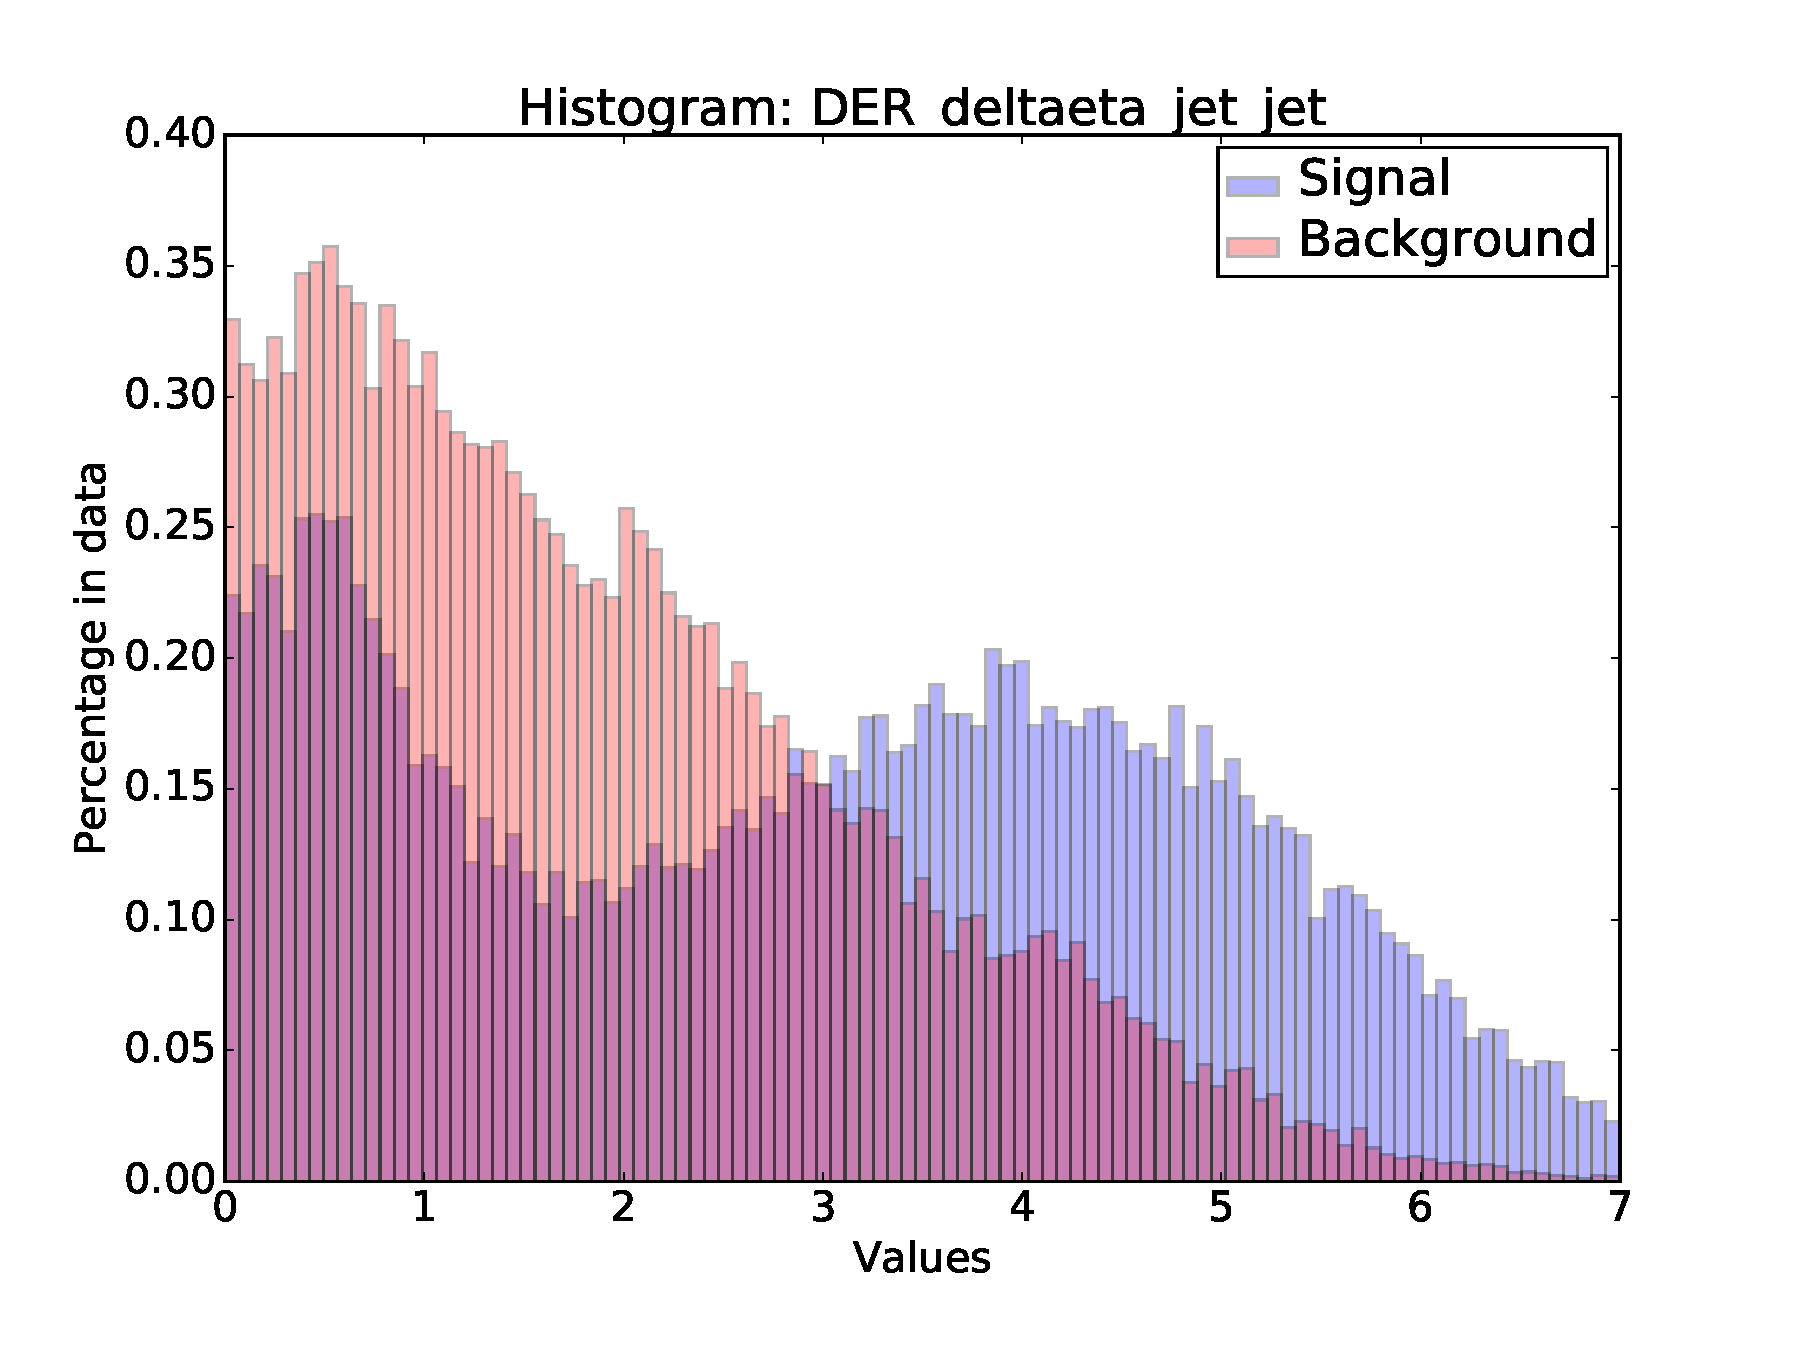
\includegraphics[width=\linewidth]{images/histogram.pdf}
  \captionof{figure}{Histogram of \emph{DER\_deltaeta\_jet\_jet}}
  \label{fig:hist1}
\end{minipage}%
\hspace{0.5em}
\begin{minipage}[t]{.49\textwidth}
  \centering
  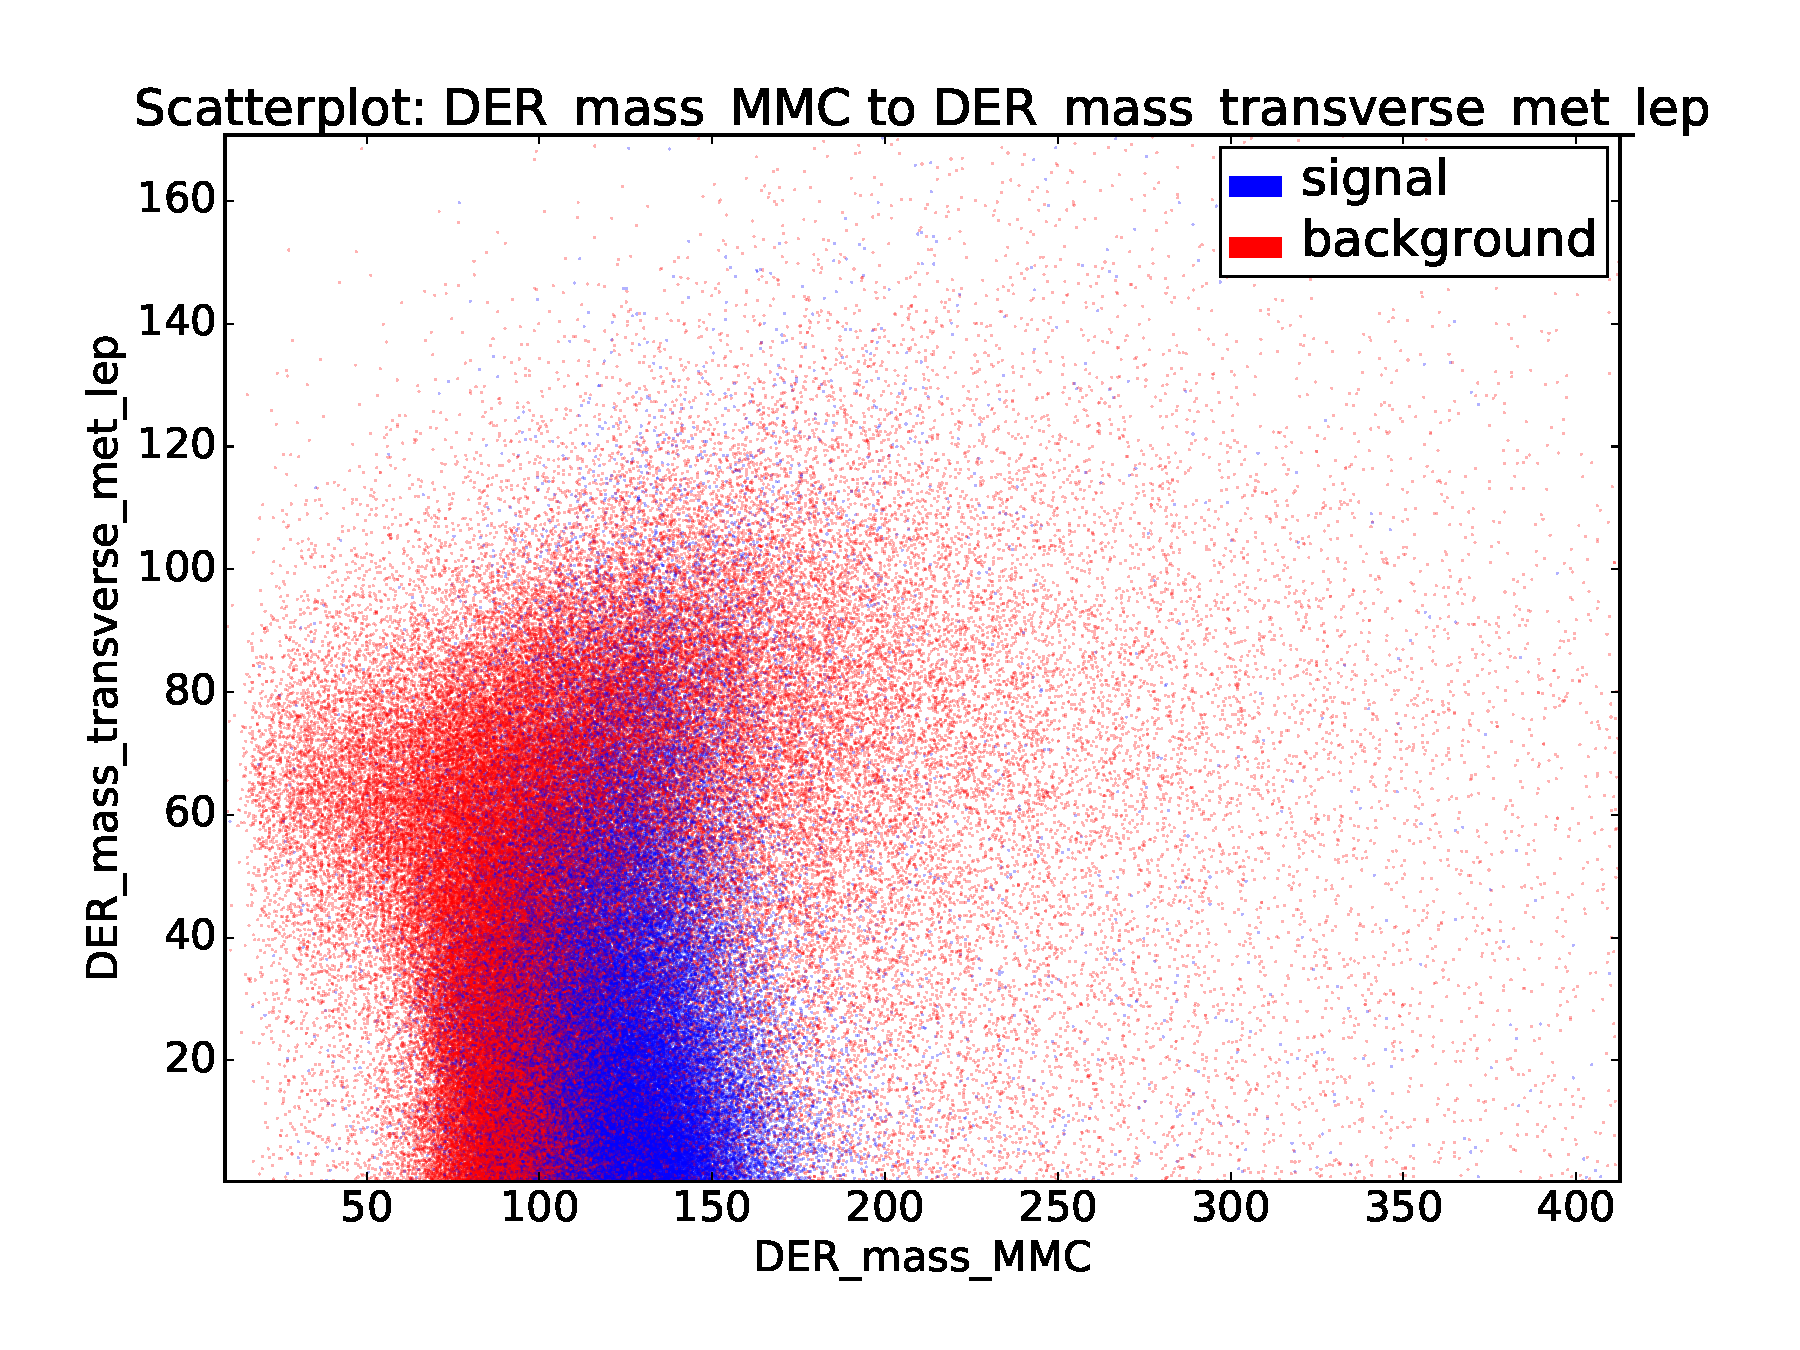
\includegraphics[width=\linewidth]{images/scatter.png}
  \captionof{figure}{Scatter plot of \emph{DER\_mass\_MMC} to \emph{DER\_mass\_transverse\_met\_lep}}
  \label{fig:scat1}
\end{minipage}
\end{figure}


\subsection{The formal problem}\label{sec:prob}
\subsection{The classification problem}\label{sec:prob}
We use the formal description of the challenge as in \cite{higgsPaper}.\\
Let $D = {(x_i,y_i,w_i)}, \ i \ \epsilon \ \{1,\ldots,n\}$ be the training sample with $n$ events, where:

\begin{itemize}
	\item $x_i \ \epsilon \ \mathbb{R}^{d}$ is a $d$-dimensional vector
	\item $y_i \ \epsilon$ \{b,s\} is the label
	\item and $w_i \ \epsilon \ \mathbb{R}^{+}$ is a non-negative weight.
\end{itemize}

The sum of signal weights
$$S = \sum_{y_i = s} w_i$$
and the sum of background weights
$$B = \sum_{y_i = b} w_i$$
represent the \emph{expected total number} of signal and background events, during the time of actual data recording.

Let a function $$g: \mathbb{R}^{d} \rightarrow \{b,s\}$$
be a binary classifier.
The set $$G_s = \{x : g(x) = s \}$$ is called the \emph{selection region}.

Our task is to find a function \emph{g} that maximizes the AMS, that we introduce in the next section.\\
For a given classifier \emph{g} we maintain an \emph{index set} 
$ \hat{G}_s = \{i : g(x_i) = s \} $ of training points that $g$ classifies as signal and an \emph{index set} $ \hat{G}_b = \{i : g(x_i) \neq s \} $. By definition each point can only be one index set, i.e. ($\hat{G}_s \cap \hat{G}_b = \emptyset$).

The index set can be turned into a submission file for the challenge, but requires to fit the following format.

\begin{verbatim}
EventId,RankOrder,Class
350000,2,b
350001,54493,s
...
899999,32455,b
\end{verbatim}

All events must have a prediction \texttt{b} or \texttt{s}. \texttt{RankOrder} shall state the probability of an event being the signal \texttt{s}, compared to all other events, e.g. rank \texttt{550000} is being considered as the most signal-like event. However, predicting the right event ranking was not necessary for the challenge.


\subsection{The evaluation}\label{sec:eval}
The evaluation of a single submission to the challenge is related to the common practice in particle physics to rate a discovery by its statistical significance, in this case 

%hier evtl mehr über die Entstehung?

\begin{equation}\label{eq:Z}
	Z = \sqrt{2 \left(n \ln{\left( \frac{n}{\mu_b} \right)} -
	n + \mu_b \right)}
\end{equation}

where $n$ is the total number of observed events and $\mu_b$ is the expected number of background-events.\\
Often in particle physics a significance of at least Z=5 (a five-sigma effect) is regarded as sufficient to claim a discovery \cite{higgsPaper}.

By estimating $n=s+b$ and $mu_b = b$ in Eq. \eqref{eq:Z}, we get the $Approximate$ $Median$ $Significance$ (AMS)

\begin{equation}\label{eq:AMS_1}
	AMS = \sqrt{2 \left( \left( s+b \right) \ln{ \left(1+ \frac{s}
	{b}  \right)} - s \right)}
\end{equation}

which is used by high-energy physicists for optimizing the selection region for stronger discovery significance \cite{higgsPaper}. 

For the challenge, a regularization-term $b_{reg}$ was introduced as an artificial shift to $b$ to decrease variance of the AMS, as this makes it easier to compare the participants if the optimal signal region was small. "The value $b_{reg}=10$ was determined using preliminary experiments." \cite{higgsPaper}

This addition to Eq. \eqref{eq:AMS_1} makes the final evaluation-formula complete:

\begin{equation}\label{eq:AMS_2}
	AMS_2 = \sqrt{2 \left( \left( s+b+b_{reg} \right) \ln{ \left(1+ \frac{s}
	{b+b_{reg}}  \right)} - s \right)}
\end{equation}

For simplicity, we will call it just AMS, as Eq. \eqref{eq:AMS_1} will not have further appearances in this thesis.

\subsubsection{The Leaderboards}
%testdata split in private and public set => KaggleSet
%weights are normalized => KaggleWeight
%compare public and private LB (graphic analysis on forums)

\subsubsection{Alternative objective functions}
For classification, a data scientist wants to train a classifier on an \textit{objective function}. Properties of the AMS (like using the logarithm) make it difficult to use it as objective function, some alternatives were proposed by the challenge-creators \cite{higgsPaper} and some challenge-participants via the Kaggle-Forum \cite{higgsForum}

\begin{itemize}
	\item alternative objective function: $ \frac{s}{\sqrt{b}} $
	\begin{itemize}
		\item only valid when $s \ll b \ and \ b \gg 1$
	\end{itemize}
\end{itemize}



\begin{equation}\label{eq:Z}
	Z = \sqrt{q_0} = \sqrt{2 \left(n \ln{\left( \frac{n}{\mu_b} \right)} -
	n + \mu_b \right)}
\end{equation}

\begin{equation}\label{eq:AMS_3}
	\frac{s}{\sqrt{b}}
\end{equation}



\eqref{eq:AMS_2}
\eqref{eq:AMS_3}
\eqref{eq:Z}



%




% Default to the notebook output style


% Inherit from the specified cell style.






    
\documentclass{article}

    
        
    
    \usepackage{graphicx} % Used to insert images
    \usepackage{adjustbox} % Used to constrain images to a maximum size 
    \usepackage{color} % Allow colors to be defined
    \usepackage{enumerate} % Needed for markdown enumerations to work
    \usepackage{geometry} % Used to adjust the document margins
    \usepackage{amsmath} % Equations
    \usepackage{amssymb} % Equations
    \usepackage{eurosym} % defines \euro
    \usepackage[mathletters]{ucs} % Extended unicode (utf-8) support
    \usepackage[utf8x]{inputenc} % Allow utf-8 characters in the tex document
    \usepackage{fancyvrb} % verbatim replacement that allows latex
    \usepackage{grffile} % extends the file name processing of package graphics 
                         % to support a larger range 
    % The hyperref package gives us a pdf with properly built
    % internal navigation ('pdf bookmarks' for the table of contents,
    % internal cross-reference links, web links for URLs, etc.)
    \usepackage{hyperref}
    \usepackage{longtable} % longtable support required by pandoc >1.10
    \usepackage{booktabs}  % table support for pandoc > 1.12.2
    

    \usepackage{tikz} % Needed to box output/input
    \usepackage{scrextend} % Used to indent output
    \usepackage{needspace} % Make prompts follow contents
    \usepackage{framed} % Used to draw output that spans multiple pages


    
    
    \definecolor{orange}{cmyk}{0,0.4,0.8,0.2}
    \definecolor{darkorange}{rgb}{.71,0.21,0.01}
    \definecolor{darkgreen}{rgb}{.12,.54,.11}
    \definecolor{myteal}{rgb}{.26, .44, .56}
    \definecolor{gray}{gray}{0.45}
    \definecolor{lightgray}{gray}{.95}
    \definecolor{mediumgray}{gray}{.8}
    \definecolor{inputbackground}{rgb}{.95, .95, .85}
    \definecolor{outputbackground}{rgb}{.95, .95, .95}
    \definecolor{traceback}{rgb}{1, .95, .95}
    % ansi colors
    \definecolor{red}{rgb}{.6,0,0}
    \definecolor{green}{rgb}{0,.65,0}
    \definecolor{brown}{rgb}{0.6,0.6,0}
    \definecolor{blue}{rgb}{0,.145,.698}
    \definecolor{purple}{rgb}{.698,.145,.698}
    \definecolor{cyan}{rgb}{0,.698,.698}
    \definecolor{lightgray}{gray}{0.5}
    
    % bright ansi colors
    \definecolor{darkgray}{gray}{0.25}
    \definecolor{lightred}{rgb}{1.0,0.39,0.28}
    \definecolor{lightgreen}{rgb}{0.48,0.99,0.0}
    \definecolor{lightblue}{rgb}{0.53,0.81,0.92}
    \definecolor{lightpurple}{rgb}{0.87,0.63,0.87}
    \definecolor{lightcyan}{rgb}{0.5,1.0,0.83}
    
    % commands and environments needed by pandoc snippets
    % extracted from the output of `pandoc -s`
    \providecommand{\tightlist}{%
      \setlength{\itemsep}{0pt}\setlength{\parskip}{0pt}}
    \DefineVerbatimEnvironment{Highlighting}{Verbatim}{commandchars=\\\{\}}
    % Add ',fontsize=\small' for more characters per line
    \newenvironment{Shaded}{}{}
    \newcommand{\KeywordTok}[1]{\textcolor[rgb]{0.00,0.44,0.13}{\textbf{{#1}}}}
    \newcommand{\DataTypeTok}[1]{\textcolor[rgb]{0.56,0.13,0.00}{{#1}}}
    \newcommand{\DecValTok}[1]{\textcolor[rgb]{0.25,0.63,0.44}{{#1}}}
    \newcommand{\BaseNTok}[1]{\textcolor[rgb]{0.25,0.63,0.44}{{#1}}}
    \newcommand{\FloatTok}[1]{\textcolor[rgb]{0.25,0.63,0.44}{{#1}}}
    \newcommand{\CharTok}[1]{\textcolor[rgb]{0.25,0.44,0.63}{{#1}}}
    \newcommand{\StringTok}[1]{\textcolor[rgb]{0.25,0.44,0.63}{{#1}}}
    \newcommand{\CommentTok}[1]{\textcolor[rgb]{0.38,0.63,0.69}{\textit{{#1}}}}
    \newcommand{\OtherTok}[1]{\textcolor[rgb]{0.00,0.44,0.13}{{#1}}}
    \newcommand{\AlertTok}[1]{\textcolor[rgb]{1.00,0.00,0.00}{\textbf{{#1}}}}
    \newcommand{\FunctionTok}[1]{\textcolor[rgb]{0.02,0.16,0.49}{{#1}}}
    \newcommand{\RegionMarkerTok}[1]{{#1}}
    \newcommand{\ErrorTok}[1]{\textcolor[rgb]{1.00,0.00,0.00}{\textbf{{#1}}}}
    \newcommand{\NormalTok}[1]{{#1}}
    
    % Define a nice break command that doesn't care if a line doesn't already
    % exist.
    \def\br{\hspace*{\fill} \\* }
    % Math Jax compatability definitions
    \def\gt{>}
    \def\lt{<}
    % Document parameters
    \title{noteAms}
    
    
    

    % Pygments definitions
    
\makeatletter
\def\PY@reset{\let\PY@it=\relax \let\PY@bf=\relax%
    \let\PY@ul=\relax \let\PY@tc=\relax%
    \let\PY@bc=\relax \let\PY@ff=\relax}
\def\PY@tok#1{\csname PY@tok@#1\endcsname}
\def\PY@toks#1+{\ifx\relax#1\empty\else%
    \PY@tok{#1}\expandafter\PY@toks\fi}
\def\PY@do#1{\PY@bc{\PY@tc{\PY@ul{%
    \PY@it{\PY@bf{\PY@ff{#1}}}}}}}
\def\PY#1#2{\PY@reset\PY@toks#1+\relax+\PY@do{#2}}

\expandafter\def\csname PY@tok@gt\endcsname{\def\PY@tc##1{\textcolor[rgb]{0.00,0.27,0.87}{##1}}}
\expandafter\def\csname PY@tok@w\endcsname{\def\PY@tc##1{\textcolor[rgb]{0.73,0.73,0.73}{##1}}}
\expandafter\def\csname PY@tok@mb\endcsname{\def\PY@tc##1{\textcolor[rgb]{0.40,0.40,0.40}{##1}}}
\expandafter\def\csname PY@tok@sh\endcsname{\def\PY@tc##1{\textcolor[rgb]{0.73,0.13,0.13}{##1}}}
\expandafter\def\csname PY@tok@go\endcsname{\def\PY@tc##1{\textcolor[rgb]{0.53,0.53,0.53}{##1}}}
\expandafter\def\csname PY@tok@mh\endcsname{\def\PY@tc##1{\textcolor[rgb]{0.40,0.40,0.40}{##1}}}
\expandafter\def\csname PY@tok@ow\endcsname{\let\PY@bf=\textbf\def\PY@tc##1{\textcolor[rgb]{0.67,0.13,1.00}{##1}}}
\expandafter\def\csname PY@tok@sx\endcsname{\def\PY@tc##1{\textcolor[rgb]{0.00,0.50,0.00}{##1}}}
\expandafter\def\csname PY@tok@mi\endcsname{\def\PY@tc##1{\textcolor[rgb]{0.40,0.40,0.40}{##1}}}
\expandafter\def\csname PY@tok@c\endcsname{\let\PY@it=\textit\def\PY@tc##1{\textcolor[rgb]{0.25,0.50,0.50}{##1}}}
\expandafter\def\csname PY@tok@s\endcsname{\def\PY@tc##1{\textcolor[rgb]{0.73,0.13,0.13}{##1}}}
\expandafter\def\csname PY@tok@nv\endcsname{\def\PY@tc##1{\textcolor[rgb]{0.10,0.09,0.49}{##1}}}
\expandafter\def\csname PY@tok@s2\endcsname{\def\PY@tc##1{\textcolor[rgb]{0.73,0.13,0.13}{##1}}}
\expandafter\def\csname PY@tok@kn\endcsname{\let\PY@bf=\textbf\def\PY@tc##1{\textcolor[rgb]{0.00,0.50,0.00}{##1}}}
\expandafter\def\csname PY@tok@sr\endcsname{\def\PY@tc##1{\textcolor[rgb]{0.73,0.40,0.53}{##1}}}
\expandafter\def\csname PY@tok@ss\endcsname{\def\PY@tc##1{\textcolor[rgb]{0.10,0.09,0.49}{##1}}}
\expandafter\def\csname PY@tok@ni\endcsname{\let\PY@bf=\textbf\def\PY@tc##1{\textcolor[rgb]{0.60,0.60,0.60}{##1}}}
\expandafter\def\csname PY@tok@sb\endcsname{\def\PY@tc##1{\textcolor[rgb]{0.73,0.13,0.13}{##1}}}
\expandafter\def\csname PY@tok@kc\endcsname{\let\PY@bf=\textbf\def\PY@tc##1{\textcolor[rgb]{0.00,0.50,0.00}{##1}}}
\expandafter\def\csname PY@tok@s1\endcsname{\def\PY@tc##1{\textcolor[rgb]{0.73,0.13,0.13}{##1}}}
\expandafter\def\csname PY@tok@gd\endcsname{\def\PY@tc##1{\textcolor[rgb]{0.63,0.00,0.00}{##1}}}
\expandafter\def\csname PY@tok@gh\endcsname{\let\PY@bf=\textbf\def\PY@tc##1{\textcolor[rgb]{0.00,0.00,0.50}{##1}}}
\expandafter\def\csname PY@tok@vc\endcsname{\def\PY@tc##1{\textcolor[rgb]{0.10,0.09,0.49}{##1}}}
\expandafter\def\csname PY@tok@gp\endcsname{\let\PY@bf=\textbf\def\PY@tc##1{\textcolor[rgb]{0.00,0.00,0.50}{##1}}}
\expandafter\def\csname PY@tok@c1\endcsname{\let\PY@it=\textit\def\PY@tc##1{\textcolor[rgb]{0.25,0.50,0.50}{##1}}}
\expandafter\def\csname PY@tok@kp\endcsname{\def\PY@tc##1{\textcolor[rgb]{0.00,0.50,0.00}{##1}}}
\expandafter\def\csname PY@tok@sc\endcsname{\def\PY@tc##1{\textcolor[rgb]{0.73,0.13,0.13}{##1}}}
\expandafter\def\csname PY@tok@nt\endcsname{\let\PY@bf=\textbf\def\PY@tc##1{\textcolor[rgb]{0.00,0.50,0.00}{##1}}}
\expandafter\def\csname PY@tok@vg\endcsname{\def\PY@tc##1{\textcolor[rgb]{0.10,0.09,0.49}{##1}}}
\expandafter\def\csname PY@tok@gu\endcsname{\let\PY@bf=\textbf\def\PY@tc##1{\textcolor[rgb]{0.50,0.00,0.50}{##1}}}
\expandafter\def\csname PY@tok@sd\endcsname{\let\PY@it=\textit\def\PY@tc##1{\textcolor[rgb]{0.73,0.13,0.13}{##1}}}
\expandafter\def\csname PY@tok@err\endcsname{\def\PY@bc##1{\setlength{\fboxsep}{0pt}\fcolorbox[rgb]{1.00,0.00,0.00}{1,1,1}{\strut ##1}}}
\expandafter\def\csname PY@tok@o\endcsname{\def\PY@tc##1{\textcolor[rgb]{0.40,0.40,0.40}{##1}}}
\expandafter\def\csname PY@tok@mo\endcsname{\def\PY@tc##1{\textcolor[rgb]{0.40,0.40,0.40}{##1}}}
\expandafter\def\csname PY@tok@gi\endcsname{\def\PY@tc##1{\textcolor[rgb]{0.00,0.63,0.00}{##1}}}
\expandafter\def\csname PY@tok@si\endcsname{\let\PY@bf=\textbf\def\PY@tc##1{\textcolor[rgb]{0.73,0.40,0.53}{##1}}}
\expandafter\def\csname PY@tok@kr\endcsname{\let\PY@bf=\textbf\def\PY@tc##1{\textcolor[rgb]{0.00,0.50,0.00}{##1}}}
\expandafter\def\csname PY@tok@mf\endcsname{\def\PY@tc##1{\textcolor[rgb]{0.40,0.40,0.40}{##1}}}
\expandafter\def\csname PY@tok@nc\endcsname{\let\PY@bf=\textbf\def\PY@tc##1{\textcolor[rgb]{0.00,0.00,1.00}{##1}}}
\expandafter\def\csname PY@tok@na\endcsname{\def\PY@tc##1{\textcolor[rgb]{0.49,0.56,0.16}{##1}}}
\expandafter\def\csname PY@tok@gr\endcsname{\def\PY@tc##1{\textcolor[rgb]{1.00,0.00,0.00}{##1}}}
\expandafter\def\csname PY@tok@ge\endcsname{\let\PY@it=\textit}
\expandafter\def\csname PY@tok@se\endcsname{\let\PY@bf=\textbf\def\PY@tc##1{\textcolor[rgb]{0.73,0.40,0.13}{##1}}}
\expandafter\def\csname PY@tok@nf\endcsname{\def\PY@tc##1{\textcolor[rgb]{0.00,0.00,1.00}{##1}}}
\expandafter\def\csname PY@tok@kt\endcsname{\def\PY@tc##1{\textcolor[rgb]{0.69,0.00,0.25}{##1}}}
\expandafter\def\csname PY@tok@cs\endcsname{\let\PY@it=\textit\def\PY@tc##1{\textcolor[rgb]{0.25,0.50,0.50}{##1}}}
\expandafter\def\csname PY@tok@gs\endcsname{\let\PY@bf=\textbf}
\expandafter\def\csname PY@tok@k\endcsname{\let\PY@bf=\textbf\def\PY@tc##1{\textcolor[rgb]{0.00,0.50,0.00}{##1}}}
\expandafter\def\csname PY@tok@vi\endcsname{\def\PY@tc##1{\textcolor[rgb]{0.10,0.09,0.49}{##1}}}
\expandafter\def\csname PY@tok@kd\endcsname{\let\PY@bf=\textbf\def\PY@tc##1{\textcolor[rgb]{0.00,0.50,0.00}{##1}}}
\expandafter\def\csname PY@tok@nl\endcsname{\def\PY@tc##1{\textcolor[rgb]{0.63,0.63,0.00}{##1}}}
\expandafter\def\csname PY@tok@ne\endcsname{\let\PY@bf=\textbf\def\PY@tc##1{\textcolor[rgb]{0.82,0.25,0.23}{##1}}}
\expandafter\def\csname PY@tok@bp\endcsname{\def\PY@tc##1{\textcolor[rgb]{0.00,0.50,0.00}{##1}}}
\expandafter\def\csname PY@tok@nb\endcsname{\def\PY@tc##1{\textcolor[rgb]{0.00,0.50,0.00}{##1}}}
\expandafter\def\csname PY@tok@il\endcsname{\def\PY@tc##1{\textcolor[rgb]{0.40,0.40,0.40}{##1}}}
\expandafter\def\csname PY@tok@nn\endcsname{\let\PY@bf=\textbf\def\PY@tc##1{\textcolor[rgb]{0.00,0.00,1.00}{##1}}}
\expandafter\def\csname PY@tok@no\endcsname{\def\PY@tc##1{\textcolor[rgb]{0.53,0.00,0.00}{##1}}}
\expandafter\def\csname PY@tok@nd\endcsname{\def\PY@tc##1{\textcolor[rgb]{0.67,0.13,1.00}{##1}}}
\expandafter\def\csname PY@tok@cp\endcsname{\def\PY@tc##1{\textcolor[rgb]{0.74,0.48,0.00}{##1}}}
\expandafter\def\csname PY@tok@cm\endcsname{\let\PY@it=\textit\def\PY@tc##1{\textcolor[rgb]{0.25,0.50,0.50}{##1}}}
\expandafter\def\csname PY@tok@m\endcsname{\def\PY@tc##1{\textcolor[rgb]{0.40,0.40,0.40}{##1}}}

\def\PYZbs{\char`\\}
\def\PYZus{\char`\_}
\def\PYZob{\char`\{}
\def\PYZcb{\char`\}}
\def\PYZca{\char`\^}
\def\PYZam{\char`\&}
\def\PYZlt{\char`\<}
\def\PYZgt{\char`\>}
\def\PYZsh{\char`\#}
\def\PYZpc{\char`\%}
\def\PYZdl{\char`\$}
\def\PYZhy{\char`\-}
\def\PYZsq{\char`\'}
\def\PYZdq{\char`\"}
\def\PYZti{\char`\~}
% for compatibility with earlier versions
\def\PYZat{@}
\def\PYZlb{[}
\def\PYZrb{]}
\makeatother


    % NB prompt colors
    \definecolor{nbframe-border}{rgb}{0.867,0.867,0.867}
    \definecolor{nbframe-bg}{rgb}{0.969,0.969,0.969}
    \definecolor{nbframe-in-prompt}{rgb}{0.0,0.0,0.502}
    \definecolor{nbframe-out-prompt}{rgb}{0.545,0.0,0.0}

    % NB prompt lengths
    \newlength{\inputpadding}
    \setlength{\inputpadding}{0.5em}
    \newlength{\cellleftmargin}
    \setlength{\cellleftmargin}{0.15\linewidth}
    \newlength{\borderthickness}
    \setlength{\borderthickness}{0.4pt}
    \newlength{\smallerfontscale}
    \setlength{\smallerfontscale}{9.5pt}

    % NB prompt font size
    \def\smaller{\fontsize{\smallerfontscale}{\smallerfontscale}\selectfont}

    % Define a background layer, in which the nb prompt shape is drawn
    \pgfdeclarelayer{background}
    \pgfsetlayers{background,main}
    \usetikzlibrary{calc}

    % define styles for the normal border and the torn border
    \tikzset{
      normal border/.style={draw=nbframe-border, fill=nbframe-bg,
        rectangle, rounded corners=2.5pt, line width=\borderthickness},
      torn border/.style={draw=white, fill=white, line width=\borderthickness}}

    % Macro to draw the shape behind the text, when it fits completly in the
    % page
    \def\notebookcellframe#1{%
    \tikz{%
      \node[inner sep=\inputpadding] (A) {#1};% Draw the text of the node
      \begin{pgfonlayer}{background}% Draw the shape behind
      \fill[normal border]%
            (A.south east) -- ($(A.south west)+(\cellleftmargin,0)$) -- 
            ($(A.north west)+(\cellleftmargin,0)$) -- (A.north east) -- cycle;
      \end{pgfonlayer}}}%

    % Macro to draw the shape, when the text will continue in next page
    \def\notebookcellframetop#1{%
    \tikz{%
      \node[inner sep=\inputpadding] (A) {#1};    % Draw the text of the node
      \begin{pgfonlayer}{background}    
      \fill[normal border]              % Draw the ``complete shape'' behind
            (A.south east) -- ($(A.south west)+(\cellleftmargin,0)$) -- 
            ($(A.north west)+(\cellleftmargin,0)$) -- (A.north east) -- cycle;
      \fill[torn border]                % Add the torn lower border
            ($(A.south east)-(0,.1)$) -- ($(A.south west)+(\cellleftmargin,-.1)$) -- 
            ($(A.south west)+(\cellleftmargin,.1)$) -- ($(A.south east)+(0,.1)$) -- cycle;
      \end{pgfonlayer}}}

    % Macro to draw the shape, when the text continues from previous page
    \def\notebookcellframebottom#1{%
    \tikz{%
      \node[inner sep=\inputpadding] (A) {#1};   % Draw the text of the node
      \begin{pgfonlayer}{background}   
      \fill[normal border]             % Draw the ``complete shape'' behind
            (A.south east) -- ($(A.south west)+(\cellleftmargin,0)$) -- 
            ($(A.north west)+(\cellleftmargin,0)$) -- (A.north east) -- cycle;
      \fill[torn border]               % Add the torn upper border
            ($(A.north east)-(0,.1)$) -- ($(A.north west)+(\cellleftmargin,-.1)$) -- 
            ($(A.north west)+(\cellleftmargin,.1)$) -- ($(A.north east)+(0,.1)$) -- cycle;
      \end{pgfonlayer}}}

    % Macro to draw the shape, when both the text continues from previous page
    % and it will continue in next page
    \def\notebookcellframemiddle#1{%
    \tikz{%
      \node[inner sep=\inputpadding] (A) {#1};   % Draw the text of the node
      \begin{pgfonlayer}{background}   
      \fill[normal border]             % Draw the ``complete shape'' behind
            (A.south east) -- ($(A.south west)+(\cellleftmargin,0)$) -- 
            ($(A.north west)+(\cellleftmargin,0)$) -- (A.north east) -- cycle;
      \fill[torn border]               % Add the torn lower border
            ($(A.south east)-(0,.1)$) -- ($(A.south west)+(\cellleftmargin,-.1)$) -- 
            ($(A.south west)+(\cellleftmargin,.1)$) -- ($(A.south east)+(0,.1)$) -- cycle;
      \fill[torn border]               % Add the torn upper border
            ($(A.north east)-(0,.1)$) -- ($(A.north west)+(\cellleftmargin,-.1)$) -- 
            ($(A.north west)+(\cellleftmargin,.1)$) -- ($(A.north east)+(0,.1)$) -- cycle;
      \end{pgfonlayer}}}

    % Define the environment which puts the frame
    % In this case, the environment also accepts an argument with an optional
    % title (which defaults to ``Example'', which is typeset in a box overlaid
    % on the top border
    \newenvironment{notebookcell}[1][0]{%
      \def\FrameCommand{\notebookcellframe}%
      \def\FirstFrameCommand{\notebookcellframetop}%
      \def\LastFrameCommand{\notebookcellframebottom}%
      \def\MidFrameCommand{\notebookcellframemiddle}%
      \par\vspace{1\baselineskip}%
      \MakeFramed {\FrameRestore}%
      \noindent\tikz\node[inner sep=0em] at ($(A.north west)-(0,0)$) {%
      
      }; 
      \par}%
    {\endMakeFramed}



    
    % Prevent overflowing lines due to hard-to-break entities
    \sloppy 
    % Setup hyperref package
    \hypersetup{
      breaklinks=true,  % so long urls are correctly broken across lines
      colorlinks=true,
      urlcolor=blue,
      linkcolor=darkorange,
      citecolor=darkgreen,
      }
    % Slightly bigger margins than the latex defaults
    
    \geometry{verbose,tmargin=1in,bmargin=1in,lmargin=1in,rmargin=1in}
    
    

    \begin{document}
    
    
    \maketitle
    
    

    %Date: 04.01.2016
    % Add contents below.

{\par%
\vspace{-1\baselineskip}%
\needspace{4\baselineskip}}%
\begin{notebookcell}[]%
\begin{addmargin}[\cellleftmargin]{0em}% left, right
{\smaller%
\par%
%
\vspace{-1\smallerfontscale}%
\begin{Verbatim}[commandchars=\\\{\}]
\PY{k+kn}{import} \PY{n+nn}{numpy} \PY{k}{as} \PY{n+nn}{np}
\PY{k+kn}{import} \PY{n+nn}{matplotlib}\PY{n+nn}{.}\PY{n+nn}{pyplot} \PY{k}{as} \PY{n+nn}{plt}
\PY{k+kn}{import} \PY{n+nn}{math}
\end{Verbatim}
%
\par%
\vspace{-1\smallerfontscale}}%
\end{addmargin}
\end{notebookcell}


    Approximate Median Significance (AMS) defined as:
\(AMS = \sqrt{2 { (s + b + b_r) log[1 + (s/(b+b_{reg}))] - s}}\)

where

\begin{itemize}
\tightlist
\item
  \(b_{reg} = 10\) is a regulization term (set by the contest),
\item
  \(b = \sum_{i=1}^{n} w_i, y_i=0\) is sum of weighted background
  (incorrectly classified as signal),
\item
  \(s = \sum_{i=1}^{n} w_i, y_i=1\) is sum of weighted signals
  (correctly classified as signal),
\item
  \(log\) is natural logarithm
\end{itemize}

    % Add contents below.

{\par%
\vspace{-1\baselineskip}%
\needspace{4\baselineskip}}%
\begin{notebookcell}[]%
\begin{addmargin}[\cellleftmargin]{0em}% left, right
{\smaller%
\par%
%
\vspace{-1\smallerfontscale}%
\begin{Verbatim}[commandchars=\\\{\}]
\PY{k}{def} \PY{n+nf}{calcAMS}\PY{p}{(}\PY{n}{s}\PY{p}{,}\PY{n}{b}\PY{p}{)}\PY{p}{:}    
    \PY{n}{br} \PY{o}{=} \PY{l+m+mf}{10.0}
    \PY{n}{radicand} \PY{o}{=} \PY{l+m+mi}{2} \PY{o}{*}\PY{p}{(} \PY{p}{(}\PY{n}{s}\PY{o}{+}\PY{n}{b}\PY{o}{+}\PY{n}{br}\PY{p}{)} \PY{o}{*} \PY{n}{math}\PY{o}{.}\PY{n}{log} \PY{p}{(}\PY{l+m+mf}{1.0} \PY{o}{+} \PY{n}{s}\PY{o}{/}\PY{p}{(}\PY{n}{b}\PY{o}{+}\PY{n}{br}\PY{p}{)}\PY{p}{)} \PY{o}{\PYZhy{}}\PY{n}{s}\PY{p}{)}
    \PY{k}{if} \PY{n}{radicand} \PY{o}{\PYZlt{}} \PY{l+m+mi}{0}\PY{p}{:}
        \PY{n+nb}{print}\PY{p}{(}\PY{l+s}{\PYZsq{}}\PY{l+s}{radicand is negative. Exiting}\PY{l+s}{\PYZsq{}}\PY{p}{)}
        \PY{n}{exit}\PY{p}{(}\PY{p}{)}
    \PY{k}{else}\PY{p}{:}
        \PY{n}{ams} \PY{o}{=} \PY{n}{math}\PY{o}{.}\PY{n}{sqrt}\PY{p}{(}\PY{n}{radicand}\PY{p}{)}
        \PY{n+nb}{print}\PY{p}{(}\PY{l+s}{\PYZdq{}}\PY{l+s}{AMS:}\PY{l+s}{\PYZdq{}}\PY{p}{,} \PY{n}{ams}\PY{p}{)}
        \PY{k}{return} \PY{n}{ams}
\end{Verbatim}
%
\par%
\vspace{-1\smallerfontscale}}%
\end{addmargin}
\end{notebookcell}


    Following this definition, we can derive a maximum AMS by simply summing
the weights of all positive labels.

    % Add contents below.

{\par%
\vspace{-1\baselineskip}%
\needspace{4\baselineskip}}%
\begin{notebookcell}[]%
\begin{addmargin}[\cellleftmargin]{0em}% left, right
{\smaller%
\par%
%
\vspace{-1\smallerfontscale}%
\begin{Verbatim}[commandchars=\\\{\}]
\PY{k}{def} \PY{n+nf}{calcWeightSums}\PY{p}{(}\PY{n}{weights}\PY{p}{,}\PY{n}{preds}\PY{p}{,}\PY{n}{labels}\PY{p}{)}\PY{p}{:}
    \PY{n}{s} \PY{o}{=} \PY{l+m+mi}{0}
    \PY{n}{b} \PY{o}{=} \PY{l+m+mi}{0}
    \PY{k}{for} \PY{n}{j} \PY{o+ow}{in} \PY{n+nb}{list}\PY{p}{(}\PY{n+nb}{range}\PY{p}{(}\PY{l+m+mi}{0}\PY{p}{,}\PY{n+nb}{len}\PY{p}{(}\PY{n}{preds}\PY{p}{)}\PY{p}{)}\PY{p}{)}\PY{p}{:}
        \PY{n}{pred} \PY{o}{=} \PY{n}{preds}\PY{p}{[}\PY{n}{j}\PY{p}{]}
        \PY{n}{label} \PY{o}{=} \PY{n}{labels}\PY{p}{[}\PY{n}{j}\PY{p}{]}
        \PY{n}{weight} \PY{o}{=} \PY{n}{weights}\PY{p}{[}\PY{n}{j}\PY{p}{]}
        \PY{k}{if} \PY{n}{pred} \PY{o}{\PYZgt{}} \PY{l+m+mf}{0.}\PY{p}{:}
            \PY{k}{if} \PY{n}{label} \PY{o}{\PYZgt{}} \PY{l+m+mf}{0.}\PY{p}{:}
                \PY{n}{s} \PY{o}{+}\PY{o}{=} \PY{n}{weight}
            \PY{k}{else}\PY{p}{:}
                \PY{n}{b} \PY{o}{+}\PY{o}{=} \PY{n}{weight}
    \PY{k}{return} \PY{n}{s}\PY{p}{,}\PY{n}{b}
\end{Verbatim}
%
\par%
\vspace{-1\smallerfontscale}}%
\end{addmargin}
\end{notebookcell}


    % Add contents below.

{\par%
\vspace{-1\baselineskip}%
\needspace{4\baselineskip}}%
\begin{notebookcell}[]%
\begin{addmargin}[\cellleftmargin]{0em}% left, right
{\smaller%
\par%
%
\vspace{-1\smallerfontscale}%
\begin{Verbatim}[commandchars=\\\{\}]
\PY{k}{def} \PY{n+nf}{calcMaxAMS}\PY{p}{(}\PY{n}{weights}\PY{p}{,}\PY{n}{labels}\PY{p}{)}\PY{p}{:}
    \PY{n}{s}\PY{p}{,}\PY{n}{b} \PY{o}{=} \PY{n}{calcWeightSums}\PY{p}{(}\PY{n}{weights}\PY{p}{,}\PY{n}{labels}\PY{p}{,}\PY{n}{labels}\PY{p}{)}
    \PY{n}{ams} \PY{o}{=} \PY{n}{calcAMS}\PY{p}{(}\PY{n}{s}\PY{p}{,}\PY{n}{b}\PY{p}{)}
    \PY{n+nb}{print}\PY{p}{(}\PY{l+s}{\PYZdq{}}\PY{l+s}{Found}\PY{l+s}{\PYZdq{}}\PY{p}{,} \PY{n+nb}{int}\PY{p}{(}\PY{n}{labels}\PY{o}{.}\PY{n}{cumsum}\PY{p}{(}\PY{p}{)}\PY{p}{[}\PY{o}{\PYZhy{}}\PY{l+m+mi}{1}\PY{p}{]}\PY{p}{)}\PY{p}{,} \PY{l+s}{\PYZdq{}}\PY{l+s}{signals.}\PY{l+s}{\PYZdq{}}\PY{p}{)}
    \PY{n+nb}{print}\PY{p}{(}\PY{l+s}{\PYZdq{}}\PY{l+s}{Weightsums signal:}\PY{l+s}{\PYZdq{}}\PY{p}{,} \PY{n}{s}\PY{p}{,} \PY{l+s}{\PYZdq{}}\PY{l+s}{| background:}\PY{l+s}{\PYZdq{}}\PY{p}{,} \PY{n}{b}\PY{p}{)}
    \PY{n+nb}{print}\PY{p}{(}\PY{l+s}{\PYZdq{}}\PY{l+s}{Maximum AMS possible with this Data:}\PY{l+s}{\PYZdq{}}\PY{p}{,} \PY{n}{ams}\PY{p}{)}
    \PY{k}{return} \PY{n}{ams}
\end{Verbatim}
%
\par%
\vspace{-1\smallerfontscale}}%
\end{addmargin}
\end{notebookcell}


    We generate AMS with good seperable toy-data, starting with the maximum
AMS. The data of the actual challenge is weighted to punish
wrong-identified signals significantly harder than wrong background. Our
toy-data will do so by using its signal-probability as weight, the
features are randomized by normal distributions.

    % Add contents below.

{\par%
\vspace{-1\baselineskip}%
\needspace{4\baselineskip}}%
\begin{notebookcell}[]%
\begin{addmargin}[\cellleftmargin]{0em}% left, right
{\smaller%
\par%
%
\vspace{-1\smallerfontscale}%
\begin{Verbatim}[commandchars=\\\{\}]
\PY{k}{def} \PY{n+nf}{generateFeature}\PY{p}{(}\PY{n}{label}\PY{p}{,} \PY{n}{mu\PYZus{}s}\PY{p}{,} \PY{n}{mu\PYZus{}b}\PY{p}{,} \PY{n}{sigma\PYZus{}s}\PY{o}{=}\PY{l+m+mi}{5}\PY{p}{,} \PY{n}{sigma\PYZus{}b}\PY{o}{=}\PY{l+m+mi}{5}\PY{p}{)}\PY{p}{:}
    \PY{k}{if} \PY{n}{label} \PY{o+ow}{is} \PY{l+m+mi}{1}\PY{p}{:}
        \PY{n}{mu} \PY{o}{=} \PY{n}{mu\PYZus{}s}
        \PY{n}{sigma} \PY{o}{=} \PY{n}{sigma\PYZus{}s}
    \PY{k}{else}\PY{p}{:}
        \PY{n}{mu} \PY{o}{=} \PY{n}{mu\PYZus{}b}
        \PY{n}{sigma} \PY{o}{=} \PY{n}{sigma\PYZus{}b}
    \PY{k}{return} \PY{n}{np}\PY{o}{.}\PY{n}{random}\PY{o}{.}\PY{n}{normal}\PY{p}{(}\PY{n}{mu}\PY{p}{,}\PY{n}{sigma}\PY{p}{)}
\end{Verbatim}
%
\par%
\vspace{-1\smallerfontscale}}%
\end{addmargin}
\end{notebookcell}


    % Add contents below.

{\par%
\vspace{-1\baselineskip}%
\needspace{4\baselineskip}}%
\begin{notebookcell}[]%
\begin{addmargin}[\cellleftmargin]{0em}% left, right
{\smaller%
\par%
%
\vspace{-1\smallerfontscale}%
\begin{Verbatim}[commandchars=\\\{\}]
\PY{k}{def} \PY{n+nf}{createToyData}\PY{p}{(}\PY{n}{n} \PY{o}{=} \PY{l+m+mi}{100}\PY{p}{,}\PY{n}{dim} \PY{o}{=} \PY{l+m+mi}{3}\PY{p}{,}\PY{n}{s\PYZus{}prob} \PY{o}{=} \PY{l+m+mf}{0.05}\PY{p}{)}\PY{p}{:}
    \PY{n}{data}\PY{o}{=} \PY{n}{np}\PY{o}{.}\PY{n}{zeros}\PY{p}{(}\PY{n}{shape} \PY{o}{=} \PY{p}{(}\PY{n}{n}\PY{p}{,}\PY{n}{dim}\PY{p}{)}\PY{p}{,}\PY{n}{dtype}\PY{o}{=}\PY{n+nb}{float}\PY{p}{)}
    \PY{k}{if} \PY{n}{dim} \PY{o}{\PYZlt{}} \PY{l+m+mi}{3}\PY{p}{:}
        \PY{n+nb}{print}\PY{p}{(}\PY{l+s}{\PYZdq{}}\PY{l+s}{Operation canceled.}\PY{l+s}{\PYZdq{}}\PY{p}{,}
              \PY{l+s}{\PYZdq{}}\PY{l+s}{Data should have at least one}\PY{l+s}{\PYZdq{}}\PY{p}{,}
              \PY{l+s}{\PYZdq{}}\PY{l+s}{additional dimension besides weights and labels.}\PY{l+s}{\PYZdq{}}\PY{p}{,}
              \PY{l+s}{\PYZdq{}}\PY{l+s}{(dim \PYZgt{}=3)}\PY{l+s}{\PYZdq{}}\PY{p}{)}
        \PY{k}{return} \PY{k}{None}
    \PY{n}{data}\PY{p}{[}\PY{p}{:}\PY{p}{,}\PY{l+m+mi}{0}\PY{p}{]} \PY{o}{=} \PY{n}{np}\PY{o}{.}\PY{n}{random}\PY{o}{.}\PY{n}{rand}\PY{p}{(}\PY{n}{n}\PY{p}{)} \PY{c}{\PYZsh{}weights}
    \PY{k}{for} \PY{n}{i} \PY{o+ow}{in} \PY{n+nb}{range}\PY{p}{(}\PY{l+m+mi}{0}\PY{p}{,}\PY{n}{n}\PY{p}{)}\PY{p}{:}
        \PY{k}{if} \PY{n}{data}\PY{p}{[}\PY{n}{i}\PY{p}{,}\PY{l+m+mi}{0}\PY{p}{]} \PY{o}{\PYZlt{}}\PY{o}{=} \PY{n}{s\PYZus{}prob}\PY{p}{:} \PY{c}{\PYZsh{} label\PYZhy{}determination}
            \PY{n}{label} \PY{o}{=} \PY{l+m+mi}{1}
        \PY{k}{else}\PY{p}{:}
            \PY{n}{label} \PY{o}{=} \PY{l+m+mi}{0}
        \PY{n}{data}\PY{p}{[}\PY{n}{i}\PY{p}{,}\PY{l+m+mi}{1}\PY{p}{]} \PY{o}{=} \PY{n}{label}
        \PY{k}{for} \PY{n}{j} \PY{o+ow}{in} \PY{n+nb}{range}\PY{p}{(}\PY{l+m+mi}{2}\PY{p}{,}\PY{n}{dim}\PY{p}{)}\PY{p}{:}
            \PY{c}{\PYZsh{}mu\PYZus{}s=j*5}
            \PY{c}{\PYZsh{}mu\PYZus{}b=j*20}
            \PY{n}{data}\PY{p}{[}\PY{n}{i}\PY{p}{,}\PY{n}{j}\PY{p}{]}\PY{o}{=}\PY{n}{generateFeature}\PY{p}{(}\PY{n}{label}\PY{p}{,}\PY{n}{mu\PYZus{}s}\PY{o}{=}\PY{p}{(}\PY{n}{j}\PY{o}{\PYZhy{}}\PY{l+m+mi}{1}\PY{p}{)}\PY{o}{*}\PY{l+m+mi}{5}\PY{p}{,}\PY{n}{mu\PYZus{}b}\PY{o}{=}\PY{p}{(}\PY{n}{j}\PY{o}{\PYZhy{}}\PY{l+m+mi}{1}\PY{p}{)}\PY{o}{*}\PY{l+m+mi}{20}\PY{p}{)}
    \PY{k}{return} \PY{n}{data}
\end{Verbatim}
%
\par%
\vspace{-1\smallerfontscale}}%
\end{addmargin}
\end{notebookcell}


    % Add contents below.

{\par%
\vspace{-1\baselineskip}%
\needspace{4\baselineskip}}%
\begin{notebookcell}[]%
\begin{addmargin}[\cellleftmargin]{0em}% left, right
{\smaller%
\par%
%
\vspace{-1\smallerfontscale}%
\begin{Verbatim}[commandchars=\\\{\}]
\PY{n}{n} \PY{o}{=} \PY{l+m+mi}{100000}
\PY{n}{prob} \PY{o}{=} \PY{l+m+mf}{0.05}
\PY{n}{data} \PY{o}{=} \PY{n}{createToyData}\PY{p}{(}\PY{n}{n}\PY{p}{,}\PY{n}{dim}\PY{o}{=}\PY{l+m+mi}{10}\PY{p}{,}\PY{n}{s\PYZus{}prob}\PY{o}{=}\PY{n}{prob}\PY{p}{)}
\end{Verbatim}
%
\par%
\vspace{-1\smallerfontscale}}%
\end{addmargin}
\end{notebookcell}


    % Add contents below.

{\par%
\vspace{-1\baselineskip}%
\needspace{4\baselineskip}}%
\begin{notebookcell}[]%
\begin{addmargin}[\cellleftmargin]{0em}% left, right
{\smaller%
\par%
%
\vspace{-1\smallerfontscale}%
\begin{Verbatim}[commandchars=\\\{\}]
\PY{n}{weights} \PY{o}{=} \PY{n}{data}\PY{p}{[}\PY{p}{:}\PY{p}{,}\PY{l+m+mi}{0}\PY{p}{]}
\PY{n}{labels} \PY{o}{=} \PY{n}{data}\PY{p}{[}\PY{p}{:}\PY{p}{,}\PY{l+m+mi}{1}\PY{p}{]}
\PY{n}{calcMaxAMS}\PY{p}{(}\PY{n}{weights}\PY{p}{,}\PY{n}{labels}\PY{p}{)}\PY{p}{;}
\end{Verbatim}
%
\par%
\vspace{-1\smallerfontscale}}%
\end{addmargin}
\end{notebookcell}


    We randomly guess labels for a solution for a second AMS with knowledge
about the toydatas signal-probability.

    % Add contents below.

{\par%
\vspace{-1\baselineskip}%
\needspace{4\baselineskip}}%
\begin{notebookcell}[]%
\begin{addmargin}[\cellleftmargin]{0em}% left, right
{\smaller%
\par%
%
\vspace{-1\smallerfontscale}%
\begin{Verbatim}[commandchars=\\\{\}]
\PY{n}{sol\PYZus{}weights} \PY{o}{=} \PY{n}{np}\PY{o}{.}\PY{n}{random}\PY{o}{.}\PY{n}{rand}\PY{p}{(}\PY{n}{n}\PY{p}{)}
\PY{n}{sol} \PY{o}{=} \PY{n}{np}\PY{o}{.}\PY{n}{zeros}\PY{p}{(}\PY{n}{n}\PY{p}{)}
\PY{k}{for} \PY{n}{i} \PY{o+ow}{in} \PY{n+nb}{range}\PY{p}{(}\PY{l+m+mi}{0}\PY{p}{,}\PY{n}{n}\PY{p}{)}\PY{p}{:}
    \PY{k}{if} \PY{n}{sol\PYZus{}weights}\PY{p}{[}\PY{n}{i}\PY{p}{]} \PY{o}{\PYZlt{}}\PY{o}{=} \PY{n}{prob}\PY{p}{:} \PY{c}{\PYZsh{} label\PYZhy{}determination}
        \PY{n}{sol}\PY{p}{[}\PY{n}{i}\PY{p}{]} \PY{o}{=} \PY{l+m+mi}{1}
    \PY{k}{else}\PY{p}{:}
        \PY{n}{sol}\PY{p}{[}\PY{n}{i}\PY{p}{]} \PY{o}{=} \PY{l+m+mi}{0}
\end{Verbatim}
%
\par%
\vspace{-1\smallerfontscale}}%
\end{addmargin}
\end{notebookcell}


    % Add contents below.

{\par%
\vspace{-1\baselineskip}%
\needspace{4\baselineskip}}%
\begin{notebookcell}[]%
\begin{addmargin}[\cellleftmargin]{0em}% left, right
{\smaller%
\par%
%
\vspace{-1\smallerfontscale}%
\begin{Verbatim}[commandchars=\\\{\}]
\PY{n}{s}\PY{p}{,}\PY{n}{b} \PY{o}{=} \PY{n}{calcWeightSums}\PY{p}{(}\PY{n}{weights}\PY{p}{,}\PY{n}{sol}\PY{p}{,}\PY{n}{labels}\PY{p}{)}
\PY{n}{calcAMS}\PY{p}{(}\PY{n}{s}\PY{p}{,}\PY{n}{b}\PY{p}{)}\PY{p}{;}
\end{Verbatim}
%
\par%
\vspace{-1\smallerfontscale}}%
\end{addmargin}
\end{notebookcell}



    % Add a bibliography block to the postdoc
    
    
    
    \end{document}

\pagebreak

\ifthenelse{ \( \equal{\zweiseitig}{twoside} \and \not \isodd{\value{page}} \)}
	{\pagebreak \thispagestyle{empty} \cleardoublepage}{\clearpage}
\section{Methods of classification}\raggedbottom
\subsection{Logistic regression}
% Add contents below.

{\par%
\vspace{-1\baselineskip}%
\needspace{4\baselineskip}}%
\begin{notebookcell}[]%
\begin{addmargin}[\cellleftmargin]{0em}% left, right
{\smaller%
\par%
%
\vspace{-1\smallerfontscale}%
\begin{Verbatim}[commandchars=\\\{\}]
\PY{k+kn}{import} \PY{n+nn}{numpy} \PY{k}{as} \PY{n+nn}{np}
\PY{k+kn}{import} \PY{n+nn}{matplotlib}\PY{n+nn}{.}\PY{n+nn}{pyplot} \PY{k}{as} \PY{n+nn}{plt}
\PY{k+kn}{import} \PY{n+nn}{math}
\PY{k+kn}{from} \PY{n+nn}{sklearn} \PY{k}{import} \PY{n}{linear\PYZus{}model} \PY{k}{as} \PY{n}{linMod}
\end{Verbatim}
%
\par%
\vspace{-1\smallerfontscale}}%
\end{addmargin}
\end{notebookcell}


    Data shall have the form of \([w,y,x_1,x_2]\) where

\begin{itemize}
\tightlist
\item
  \(w\) is a weight in the intervall \([0,1)\)
\item
  \(y\) is the label ``0'' for ``background'' or ``1'' for ``signal''
\item
  \(x_n\) are randomly generated features with respect to the label
\end{itemize}

    % Add contents below.

{\par%
\vspace{-1\baselineskip}%
\needspace{4\baselineskip}}%
\begin{notebookcell}[]%
\begin{addmargin}[\cellleftmargin]{0em}% left, right
{\smaller%
\par%
%
\vspace{-1\smallerfontscale}%
\begin{Verbatim}[commandchars=\\\{\}]
\PY{k}{def} \PY{n+nf}{generateFeature}\PY{p}{(}\PY{n}{label}\PY{p}{,} \PY{n}{mu\PYZus{}s}\PY{p}{,} \PY{n}{mu\PYZus{}b}\PY{p}{,} \PY{n}{sigma\PYZus{}s}\PY{o}{=}\PY{l+m+mi}{5}\PY{p}{,} \PY{n}{sigma\PYZus{}b}\PY{o}{=}\PY{l+m+mi}{5}\PY{p}{)}\PY{p}{:}
    \PY{k}{if} \PY{n}{label} \PY{o+ow}{is} \PY{l+m+mi}{1}\PY{p}{:}
        \PY{n}{mu} \PY{o}{=} \PY{n}{mu\PYZus{}s}
        \PY{n}{sigma} \PY{o}{=} \PY{n}{sigma\PYZus{}s}
    \PY{k}{else}\PY{p}{:}
        \PY{n}{mu} \PY{o}{=} \PY{n}{mu\PYZus{}b}
        \PY{n}{sigma} \PY{o}{=} \PY{n}{sigma\PYZus{}b}
    \PY{k}{return} \PY{n}{np}\PY{o}{.}\PY{n}{random}\PY{o}{.}\PY{n}{normal}\PY{p}{(}\PY{n}{mu}\PY{p}{,}\PY{n}{sigma}\PY{p}{)}
\end{Verbatim}
%
\par%
\vspace{-1\smallerfontscale}}%
\end{addmargin}
\end{notebookcell}


    Approximate Median Significance (AMS) defined as:

\[AMS = \sqrt{2 { (s + b + b_r) log[1 + (s/(b+b_{reg}))] - s}}\]

where

\begin{itemize}
\tightlist
\item
  \(b_{reg} = 10\) is a regulization term (set by the contest),
\item
  \(b = \sum_{i=1}^{n} w_i, y_i=0\) is sum of weighted background
  (incorrectly classified as signal),
\item
  \(s = \sum_{i=1}^{n} w_i, y_i=1\) is sum of weighted signals
  (correctly classified as signal),
\item
  \(log\) is natural logarithm
\end{itemize}

    % Add contents below.

{\par%
\vspace{-1\baselineskip}%
\needspace{4\baselineskip}}%
\begin{notebookcell}[]%
\begin{addmargin}[\cellleftmargin]{0em}% left, right
{\smaller%
\par%
%
\vspace{-1\smallerfontscale}%
\begin{Verbatim}[commandchars=\\\{\}]
\PY{k}{def} \PY{n+nf}{calcAMS}\PY{p}{(}\PY{n}{s}\PY{p}{,}\PY{n}{b}\PY{p}{)}\PY{p}{:}    
    \PY{n}{br} \PY{o}{=} \PY{l+m+mf}{10.0}
    \PY{n}{radicand} \PY{o}{=} \PY{l+m+mi}{2} \PY{o}{*}\PY{p}{(} \PY{p}{(}\PY{n}{s}\PY{o}{+}\PY{n}{b}\PY{o}{+}\PY{n}{br}\PY{p}{)} \PY{o}{*} \PY{n}{math}\PY{o}{.}\PY{n}{log} \PY{p}{(}\PY{l+m+mf}{1.0} \PY{o}{+} \PY{n}{s}\PY{o}{/}\PY{p}{(}\PY{n}{b}\PY{o}{+}\PY{n}{br}\PY{p}{)}\PY{p}{)} \PY{o}{\PYZhy{}}\PY{n}{s}\PY{p}{)}
    \PY{k}{if} \PY{n}{radicand} \PY{o}{\PYZlt{}} \PY{l+m+mi}{0}\PY{p}{:}
        \PY{n+nb}{print}\PY{p}{(}\PY{l+s}{\PYZsq{}}\PY{l+s}{radicand is negative. Exiting}\PY{l+s}{\PYZsq{}}\PY{p}{)}
        \PY{n}{exit}\PY{p}{(}\PY{p}{)}
    \PY{k}{else}\PY{p}{:}
        \PY{k}{return} \PY{n}{math}\PY{o}{.}\PY{n}{sqrt}\PY{p}{(}\PY{n}{radicand}\PY{p}{)}
\end{Verbatim}
%
\par%
\vspace{-1\smallerfontscale}}%
\end{addmargin}
\end{notebookcell}


    % Add contents below.

{\par%
\vspace{-1\baselineskip}%
\needspace{4\baselineskip}}%
\begin{notebookcell}[]%
\begin{addmargin}[\cellleftmargin]{0em}% left, right
{\smaller%
\par%
%
\vspace{-1\smallerfontscale}%
\begin{Verbatim}[commandchars=\\\{\}]
\PY{k}{def} \PY{n+nf}{calcWeightSums}\PY{p}{(}\PY{n}{weights}\PY{p}{,}\PY{n}{preds}\PY{p}{,}\PY{n}{labels}\PY{p}{)}\PY{p}{:}
    \PY{n}{s} \PY{o}{=} \PY{l+m+mi}{0}
    \PY{n}{b} \PY{o}{=} \PY{l+m+mi}{0}
    \PY{k}{for} \PY{n}{j} \PY{o+ow}{in} \PY{n+nb}{list}\PY{p}{(}\PY{n+nb}{range}\PY{p}{(}\PY{l+m+mi}{0}\PY{p}{,}\PY{n+nb}{len}\PY{p}{(}\PY{n}{preds}\PY{p}{)}\PY{p}{)}\PY{p}{)}\PY{p}{:}
        \PY{n}{pred} \PY{o}{=} \PY{n}{preds}\PY{p}{[}\PY{n}{j}\PY{p}{]}
        \PY{n}{label} \PY{o}{=} \PY{n}{labels}\PY{p}{[}\PY{n}{j}\PY{p}{]}
        \PY{n}{weight} \PY{o}{=} \PY{n}{weights}\PY{p}{[}\PY{n}{j}\PY{p}{]}
        \PY{k}{if} \PY{n}{pred} \PY{o}{\PYZgt{}} \PY{l+m+mf}{0.}\PY{p}{:}
            \PY{k}{if} \PY{n}{label} \PY{o}{\PYZgt{}} \PY{l+m+mf}{0.}\PY{p}{:}
                \PY{n}{s} \PY{o}{+}\PY{o}{=} \PY{n}{weight}
            \PY{k}{else}\PY{p}{:}
                \PY{n}{b} \PY{o}{+}\PY{o}{=} \PY{n}{weight}
    \PY{k}{return} \PY{n}{s}\PY{p}{,}\PY{n}{b}
\end{Verbatim}
%
\par%
\vspace{-1\smallerfontscale}}%
\end{addmargin}
\end{notebookcell}


    actually generate data

    % Add contents below.

{\par%
\vspace{-1\baselineskip}%
\needspace{4\baselineskip}}%
\begin{notebookcell}[]%
\begin{addmargin}[\cellleftmargin]{0em}% left, right
{\smaller%
\par%
%
\vspace{-1\smallerfontscale}%
\begin{Verbatim}[commandchars=\\\{\}]
\PY{c}{\PYZsh{}toydata shall have n vectors with 5 dimensions}
\PY{n}{n} \PY{o}{=} \PY{l+m+mi}{100000}
\PY{c}{\PYZsh{}probability for signal\PYZhy{}label}
\PY{n}{s\PYZus{}prob} \PY{o}{=} \PY{l+m+mf}{0.05}
\PY{c}{\PYZsh{}random values will be used as weights for evaluation later}
\PY{n}{weights} \PY{o}{=} \PY{n}{np}\PY{o}{.}\PY{n}{random}\PY{o}{.}\PY{n}{rand}\PY{p}{(}\PY{n}{n}\PY{p}{)}
\PY{n}{labels} \PY{o}{=} \PY{n}{np}\PY{o}{.}\PY{n}{zeros}\PY{p}{(}\PY{n}{n}\PY{p}{)}
\PY{n}{x\PYZus{}1} \PY{o}{=} \PY{n}{np}\PY{o}{.}\PY{n}{zeros}\PY{p}{(}\PY{n}{n}\PY{p}{)}
\PY{n}{x\PYZus{}2} \PY{o}{=} \PY{n}{np}\PY{o}{.}\PY{n}{zeros}\PY{p}{(}\PY{n}{n}\PY{p}{)}

\PY{k}{for} \PY{n}{i} \PY{o+ow}{in} \PY{n+nb}{range}\PY{p}{(}\PY{l+m+mi}{0}\PY{p}{,}\PY{n}{n}\PY{p}{)}\PY{p}{:}
    \PY{k}{if} \PY{n}{weights}\PY{p}{[}\PY{n}{i}\PY{p}{]} \PY{o}{\PYZlt{}}\PY{o}{=} \PY{n}{s\PYZus{}prob}\PY{p}{:}
        \PY{n}{label} \PY{o}{=} \PY{l+m+mi}{1}
    \PY{k}{else}\PY{p}{:}
        \PY{n}{label} \PY{o}{=} \PY{l+m+mi}{0}
    \PY{n}{labels}\PY{p}{[}\PY{n}{i}\PY{p}{]} \PY{o}{=} \PY{n}{label}
    \PY{n}{x\PYZus{}1}\PY{p}{[}\PY{n}{i}\PY{p}{]}\PY{o}{=}\PY{n}{generateFeature}\PY{p}{(}\PY{n}{label}\PY{p}{,}\PY{n}{mu\PYZus{}s}\PY{o}{=}\PY{l+m+mi}{5}\PY{p}{,}\PY{n}{mu\PYZus{}b}\PY{o}{=}\PY{l+m+mi}{20}\PY{p}{)}
    \PY{n}{x\PYZus{}2}\PY{p}{[}\PY{n}{i}\PY{p}{]}\PY{o}{=}\PY{n}{generateFeature}\PY{p}{(}\PY{n}{label}\PY{p}{,}\PY{n}{mu\PYZus{}s}\PY{o}{=}\PY{l+m+mi}{5}\PY{p}{,}\PY{n}{mu\PYZus{}b}\PY{o}{=}\PY{l+m+mi}{25}\PY{p}{)}
\end{Verbatim}
%
\par%
\vspace{-1\smallerfontscale}}%
\end{addmargin}
\end{notebookcell}


    visualize

    % Add contents below.

{\par%
\vspace{-1\baselineskip}%
\needspace{4\baselineskip}}%
\begin{notebookcell}[]%
\begin{addmargin}[\cellleftmargin]{0em}% left, right
{\smaller%
\par%
%
\vspace{-1\smallerfontscale}%
\begin{Verbatim}[commandchars=\\\{\}]
\PY{o}{\PYZpc{}}\PY{k}{pylab} inline
\PY{n}{plt}\PY{o}{.}\PY{n}{scatter}\PY{p}{(}\PY{n}{x\PYZus{}1}\PY{p}{,} \PY{n}{x\PYZus{}2}\PY{p}{,} \PY{n}{edgecolor}\PY{o}{=}\PY{l+s}{\PYZdq{}}\PY{l+s}{\PYZdq{}}\PY{p}{,} \PY{n}{c}\PY{o}{=}\PY{n}{labels}\PY{p}{,} \PY{n}{alpha}\PY{o}{=}\PY{l+m+mf}{0.5}\PY{p}{)}
\end{Verbatim}
%
\par%
\vspace{-1\smallerfontscale}}%
\end{addmargin}
\end{notebookcell}


    % Add contents below.

{\par%
\vspace{-1\baselineskip}%
\needspace{4\baselineskip}}%
\begin{notebookcell}[]%
\begin{addmargin}[\cellleftmargin]{0em}% left, right
{\smaller%
\par%
%
\vspace{-1\smallerfontscale}%
\begin{Verbatim}[commandchars=\\\{\}]
\PY{k}{def} \PY{n+nf}{splitList}\PY{p}{(}\PY{n}{xList}\PY{p}{,}\PY{n}{n}\PY{p}{)}\PY{p}{:}
    \PY{n}{aList} \PY{o}{=} \PY{n}{xList}\PY{p}{[}\PY{p}{:}\PY{n}{n}\PY{p}{]}
    \PY{n}{bList} \PY{o}{=} \PY{n}{xList}\PY{p}{[}\PY{n}{n}\PY{p}{:}\PY{p}{]}
    \PY{k}{return} \PY{n}{aList}\PY{p}{,}\PY{n}{bList}
\end{Verbatim}
%
\par%
\vspace{-1\smallerfontscale}}%
\end{addmargin}
\end{notebookcell}


    split toydata into training- and testset for the classifier

    % Add contents below.

{\par%
\vspace{-1\baselineskip}%
\needspace{4\baselineskip}}%
\begin{notebookcell}[]%
\begin{addmargin}[\cellleftmargin]{0em}% left, right
{\smaller%
\par%
%
\vspace{-1\smallerfontscale}%
\begin{Verbatim}[commandchars=\\\{\}]
\PY{n}{n\PYZus{}train} \PY{o}{=} \PY{n+nb}{int}\PY{p}{(}\PY{n}{n}\PY{o}{/}\PY{l+m+mi}{10}\PY{p}{)}

\PY{n}{train\PYZus{}x\PYZus{}1}\PY{p}{,}\PY{n}{test\PYZus{}x\PYZus{}1} \PY{o}{=} \PY{n}{splitList}\PY{p}{(}\PY{n}{x\PYZus{}1}\PY{p}{,}\PY{n}{n\PYZus{}train}\PY{p}{)}
\PY{n}{train\PYZus{}x\PYZus{}2}\PY{p}{,}\PY{n}{test\PYZus{}x\PYZus{}2} \PY{o}{=} \PY{n}{splitList}\PY{p}{(}\PY{n}{x\PYZus{}2}\PY{p}{,}\PY{n}{n\PYZus{}train}\PY{p}{)}
\PY{n}{train\PYZus{}labels}\PY{p}{,}\PY{n}{test\PYZus{}labels} \PY{o}{=} \PY{n}{splitList}\PY{p}{(}\PY{n}{labels}\PY{p}{,}\PY{n}{n\PYZus{}train}\PY{p}{)}
\PY{n}{test\PYZus{}weights} \PY{o}{=} \PY{n}{splitList}\PY{p}{(}\PY{n}{weights}\PY{p}{,}\PY{n}{n\PYZus{}train}\PY{p}{)}\PY{p}{[}\PY{l+m+mi}{1}\PY{p}{]}
\end{Verbatim}
%
\par%
\vspace{-1\smallerfontscale}}%
\end{addmargin}
\end{notebookcell}


    For Comparison, we calculate the best possible AMS\\
(case: every signal correctly detected)

    % Add contents below.

{\par%
\vspace{-1\baselineskip}%
\needspace{4\baselineskip}}%
\begin{notebookcell}[]%
\begin{addmargin}[\cellleftmargin]{0em}% left, right
{\smaller%
\par%
%
\vspace{-1\smallerfontscale}%
\begin{Verbatim}[commandchars=\\\{\}]
\PY{k}{def} \PY{n+nf}{calcMaxAMS}\PY{p}{(}\PY{n}{weights}\PY{p}{,}\PY{n}{labels}\PY{p}{)}\PY{p}{:}
    \PY{n}{s}\PY{p}{,}\PY{n}{b} \PY{o}{=} \PY{n}{calcWeightSums}\PY{p}{(}\PY{n}{weights}\PY{p}{,}\PY{n}{labels}\PY{p}{,}\PY{n}{labels}\PY{p}{)}
    \PY{n}{ams} \PY{o}{=} \PY{n}{calcAMS}\PY{p}{(}\PY{n}{s}\PY{p}{,}\PY{n}{b}\PY{p}{)}
    \PY{n+nb}{print}\PY{p}{(}\PY{l+s}{\PYZdq{}}\PY{l+s}{Maximum AMS possible with this Data:}\PY{l+s}{\PYZdq{}}\PY{p}{,} \PY{n}{ams}\PY{p}{)}
    \PY{k}{return} \PY{n}{ams}
\end{Verbatim}
%
\par%
\vspace{-1\smallerfontscale}}%
\end{addmargin}
\end{notebookcell}


    % Add contents below.

{\par%
\vspace{-1\baselineskip}%
\needspace{4\baselineskip}}%
\begin{notebookcell}[]%
\begin{addmargin}[\cellleftmargin]{0em}% left, right
{\smaller%
\par%
%
\vspace{-1\smallerfontscale}%
\begin{Verbatim}[commandchars=\\\{\}]
\PY{n}{calcMaxAMS}\PY{p}{(}\PY{n}{test\PYZus{}weights}\PY{p}{,}\PY{n}{test\PYZus{}labels}\PY{p}{)}\PY{p}{;}
\end{Verbatim}
%
\par%
\vspace{-1\smallerfontscale}}%
\end{addmargin}
\end{notebookcell}


    we initialize the Logistic Regression Classifier, shape the input-data
and fit the model

    % Add contents below.

{\par%
\vspace{-1\baselineskip}%
\needspace{4\baselineskip}}%
\begin{notebookcell}[]%
\begin{addmargin}[\cellleftmargin]{0em}% left, right
{\smaller%
\par%
%
\vspace{-1\smallerfontscale}%
\begin{Verbatim}[commandchars=\\\{\}]
\PY{n}{logReg} \PY{o}{=} \PY{n}{linMod}\PY{o}{.}\PY{n}{LogisticRegression}\PY{p}{(}\PY{n}{C}\PY{o}{=}\PY{l+m+mi}{1}\PY{n}{e5}\PY{p}{)}

\PY{n}{train\PYZus{}x} \PY{o}{=} \PY{n}{np}\PY{o}{.}\PY{n}{array}\PY{p}{(}\PY{p}{[}\PY{n}{train\PYZus{}x\PYZus{}1}\PY{p}{,}\PY{n}{train\PYZus{}x\PYZus{}2}\PY{p}{]}\PY{p}{)}\PY{o}{.}\PY{n}{transpose}\PY{p}{(}\PY{p}{)}
\PY{n}{test\PYZus{}x} \PY{o}{=} \PY{n}{np}\PY{o}{.}\PY{n}{array}\PY{p}{(}\PY{p}{[}\PY{n}{test\PYZus{}x\PYZus{}1}\PY{p}{,}\PY{n}{test\PYZus{}x\PYZus{}2}\PY{p}{]}\PY{p}{)}\PY{o}{.}\PY{n}{transpose}\PY{p}{(}\PY{p}{)}
\PY{n}{train\PYZus{}labels} \PY{o}{=} \PY{n}{np}\PY{o}{.}\PY{n}{array}\PY{p}{(}\PY{n}{train\PYZus{}labels}\PY{p}{)}\PY{o}{.}\PY{n}{transpose}\PY{p}{(}\PY{p}{)}
\PY{n}{test\PYZus{}labels} \PY{o}{=} \PY{n}{np}\PY{o}{.}\PY{n}{array}\PY{p}{(}\PY{n}{test\PYZus{}labels}\PY{p}{)}\PY{o}{.}\PY{n}{transpose}\PY{p}{(}\PY{p}{)}

\PY{n}{logReg}\PY{o}{.}\PY{n}{fit}\PY{p}{(}\PY{n}{train\PYZus{}x}\PY{p}{,}\PY{n}{train\PYZus{}labels}\PY{p}{)}

\PY{n}{logReg}\PY{o}{.}\PY{n}{sparsify}\PY{p}{(}\PY{p}{)}

\PY{n}{predProb} \PY{o}{=} \PY{n}{logReg}\PY{o}{.}\PY{n}{predict\PYZus{}proba}\PY{p}{(}\PY{n}{test\PYZus{}x}\PY{p}{)}
\PY{n}{pred} \PY{o}{=} \PY{n}{logReg}\PY{o}{.}\PY{n}{predict}\PY{p}{(}\PY{n}{test\PYZus{}x}\PY{p}{)}
\PY{n}{score} \PY{o}{=} \PY{n}{logReg}\PY{o}{.}\PY{n}{score}\PY{p}{(}\PY{n}{test\PYZus{}x}\PY{p}{,}\PY{n}{test\PYZus{}labels}\PY{p}{)}

\PY{n+nb}{print}\PY{p}{(}\PY{l+s}{\PYZdq{}}\PY{l+s}{Score:}\PY{l+s}{\PYZdq{}}\PY{p}{,} \PY{n}{score}\PY{p}{)}
\end{Verbatim}
%
\par%
\vspace{-1\smallerfontscale}}%
\end{addmargin}
\end{notebookcell}


    % Add contents below.

{\par%
\vspace{-1\baselineskip}%
\needspace{4\baselineskip}}%
\begin{notebookcell}[]%
\begin{addmargin}[\cellleftmargin]{0em}% left, right
{\smaller%
\par%
%
\vspace{-1\smallerfontscale}%
\begin{Verbatim}[commandchars=\\\{\}]
\PY{n}{s}\PY{p}{,}\PY{n}{b} \PY{o}{=} \PY{n}{calcWeightSums}\PY{p}{(}\PY{n}{test\PYZus{}weights}\PY{p}{,}\PY{n}{pred}\PY{p}{,}\PY{n}{test\PYZus{}labels}\PY{p}{)}
\PY{n}{calcAMS}\PY{p}{(}\PY{n}{s}\PY{p}{,}\PY{n}{b}\PY{p}{)}
\end{Verbatim}
%
\par%
\vspace{-1\smallerfontscale}}%
\end{addmargin}
\end{notebookcell}


    We successfully tested logistic Regression, now let's use it on actual
CERN-Data.

    % Add contents below.

{\par%
\vspace{-1\baselineskip}%
\needspace{4\baselineskip}}%
\begin{notebookcell}[]%
\begin{addmargin}[\cellleftmargin]{0em}% left, right
{\smaller%
\par%
%
\vspace{-1\smallerfontscale}%
\begin{Verbatim}[commandchars=\\\{\}]
\PY{k+kn}{import} \PY{n+nn}{KaggleData}\PY{p}{;}
\end{Verbatim}
%
\par%
\vspace{-1\smallerfontscale}}%
\end{addmargin}
\end{notebookcell}


    % Add contents below.

{\par%
\vspace{-1\baselineskip}%
\needspace{4\baselineskip}}%
\begin{notebookcell}[]%
\begin{addmargin}[\cellleftmargin]{0em}% left, right
{\smaller%
\par%
%
\vspace{-1\smallerfontscale}%
\begin{Verbatim}[commandchars=\\\{\}]
\PY{n}{csvDict}\PY{p}{,}\PY{n}{header} \PY{o}{=} \PY{n}{KaggleData}\PY{o}{.}\PY{n}{createCsvDictionary}\PY{p}{(}\PY{p}{)}
\end{Verbatim}
%
\par%
\vspace{-1\smallerfontscale}}%
\end{addmargin}
\end{notebookcell}


    Trainingset has key ``t''\\
Public Testset has key ``p'' (note: ``p'' won't work, using private
Testset (``v''))

    % Add contents below.

{\par%
\vspace{-1\baselineskip}%
\needspace{4\baselineskip}}%
\begin{notebookcell}[]%
\begin{addmargin}[\cellleftmargin]{0em}% left, right
{\smaller%
\par%
%
\vspace{-1\smallerfontscale}%
\begin{Verbatim}[commandchars=\\\{\}]
\PY{k}{def} \PY{n+nf}{getFeatureSets}\PY{p}{(}\PY{n}{featureName}\PY{p}{)}\PY{p}{:}
    \PY{n}{trainFeature} \PY{o}{=} \PY{n}{KaggleData}\PY{o}{.}\PY{n}{getFeatureAsNpArray}\PY{p}{(}
        \PY{n}{csvDict}\PY{p}{,}\PY{n}{header}\PY{p}{,}\PY{n}{featureName}\PY{p}{,}\PY{p}{[}\PY{l+s}{\PYZdq{}}\PY{l+s}{t}\PY{l+s}{\PYZdq{}}\PY{p}{]}\PY{p}{,}\PY{n}{hasErrorValues} \PY{o}{=} \PY{k}{True}\PY{p}{)}
    \PY{n}{testFeature} \PY{o}{=} \PY{n}{KaggleData}\PY{o}{.}\PY{n}{getFeatureAsNpArray}\PY{p}{(}
        \PY{n}{csvDict}\PY{p}{,}\PY{n}{header}\PY{p}{,}\PY{n}{featureName}\PY{p}{,}\PY{p}{[}\PY{l+s}{\PYZdq{}}\PY{l+s}{v}\PY{l+s}{\PYZdq{}}\PY{p}{]}\PY{p}{,}\PY{n}{hasErrorValues} \PY{o}{=} \PY{k}{True}\PY{p}{)}
    \PY{k}{return} \PY{n}{trainFeature}\PY{p}{,} \PY{n}{testFeature}
\end{Verbatim}
%
\par%
\vspace{-1\smallerfontscale}}%
\end{addmargin}
\end{notebookcell}


    % Add contents below.

{\par%
\vspace{-1\baselineskip}%
\needspace{4\baselineskip}}%
\begin{notebookcell}[]%
\begin{addmargin}[\cellleftmargin]{0em}% left, right
{\smaller%
\par%
%
\vspace{-1\smallerfontscale}%
\begin{Verbatim}[commandchars=\\\{\}]
\PY{n}{train\PYZus{}eventList}\PY{p}{,}\PY{n}{test\PYZus{}eventList} \PY{o}{=} \PY{n}{getFeatureSets}\PY{p}{(}\PY{l+s}{\PYZdq{}}\PY{l+s}{EventId}\PY{l+s}{\PYZdq{}}\PY{p}{)}
\PY{n}{train\PYZus{}labels}\PY{p}{,}\PY{n}{test\PYZus{}labels} \PY{o}{=} \PY{n}{getFeatureSets}\PY{p}{(}\PY{l+s}{\PYZdq{}}\PY{l+s}{Label}\PY{l+s}{\PYZdq{}}\PY{p}{)}
\PY{n}{test\PYZus{}weights} \PY{o}{=} \PY{n}{getFeatureSets}\PY{p}{(}\PY{l+s}{\PYZdq{}}\PY{l+s}{KaggleWeight}\PY{l+s}{\PYZdq{}}\PY{p}{)}\PY{p}{[}\PY{l+m+mi}{1}\PY{p}{]}
\end{Verbatim}
%
\par%
\vspace{-1\smallerfontscale}}%
\end{addmargin}
\end{notebookcell}


    We observe the relation Label \textless{}=\textgreater{} Weight

    % Add contents below.

{\par%
\vspace{-1\baselineskip}%
\needspace{4\baselineskip}}%
\begin{notebookcell}[]%
\begin{addmargin}[\cellleftmargin]{0em}% left, right
{\smaller%
\par%
%
\vspace{-1\smallerfontscale}%
\begin{Verbatim}[commandchars=\\\{\}]
\PY{n}{signal\PYZus{}sum} \PY{o}{=} \PY{n+nb}{int}\PY{p}{(}\PY{n}{test\PYZus{}labels}\PY{o}{.}\PY{n}{cumsum}\PY{p}{(}\PY{p}{)}\PY{p}{[}\PY{o}{\PYZhy{}}\PY{l+m+mi}{1}\PY{p}{]}\PY{p}{)}
\PY{n}{background\PYZus{}sum} \PY{o}{=} \PY{n+nb}{int}\PY{p}{(}\PY{n+nb}{len}\PY{p}{(}\PY{n}{test\PYZus{}labels}\PY{p}{)}\PY{o}{\PYZhy{}}\PY{n}{signal\PYZus{}sum}\PY{p}{)}
\PY{n}{signal\PYZus{}weight} \PY{o}{=} \PY{l+m+mi}{0}
\PY{n}{background\PYZus{}weight} \PY{o}{=} \PY{l+m+mi}{0}
\PY{k}{for} \PY{n}{i} \PY{o+ow}{in} \PY{n+nb}{range}\PY{p}{(}\PY{l+m+mi}{0}\PY{p}{,}\PY{n+nb}{len}\PY{p}{(}\PY{n}{test\PYZus{}labels}\PY{p}{)}\PY{p}{)}\PY{p}{:}
    \PY{k}{if} \PY{n}{test\PYZus{}labels}\PY{p}{[}\PY{n}{i}\PY{p}{]} \PY{o}{\PYZgt{}} \PY{l+m+mi}{0}\PY{p}{:}
        \PY{n}{signal\PYZus{}weight} \PY{o}{+}\PY{o}{=} \PY{n}{test\PYZus{}weights}\PY{p}{[}\PY{n}{i}\PY{p}{]}
    \PY{k}{else}\PY{p}{:}
        \PY{n}{background\PYZus{}weight} \PY{o}{+}\PY{o}{=} \PY{n}{test\PYZus{}weights}\PY{p}{[}\PY{n}{i}\PY{p}{]}
\PY{n+nb}{print}\PY{p}{(}\PY{n}{background\PYZus{}weight}\PY{o}{/}\PY{n}{background\PYZus{}sum}\PY{p}{)}
\PY{n+nb}{print}\PY{p}{(}\PY{n}{signal\PYZus{}weight}\PY{o}{/}\PY{n}{signal\PYZus{}sum}\PY{p}{)}
\end{Verbatim}
%
\par%
\vspace{-1\smallerfontscale}}%
\end{addmargin}
\end{notebookcell}


    We can observe, that False signals will be weighted a lot heavier than
True signals.

If a classifier achieved a higher AMS while detecting less signals,\\
we can make statements about the usabilty of the features, the
classifier used.

We choose features with beneficial properties for classifying.

    % Add contents below.

{\par%
\vspace{-1\baselineskip}%
\needspace{4\baselineskip}}%
\begin{notebookcell}[]%
\begin{addmargin}[\cellleftmargin]{0em}% left, right
{\smaller%
\par%
%
\vspace{-1\smallerfontscale}%
\begin{Verbatim}[commandchars=\\\{\}]
\PY{p}{(}\PY{n}{train\PYZus{}DER\PYZus{}met\PYZus{}phi\PYZus{}centrality}\PY{p}{,}
 \PY{n}{test\PYZus{}DER\PYZus{}met\PYZus{}phi\PYZus{}centrality}\PY{p}{)} \PY{o}{=} \PY{n}{getFeatureSets}\PY{p}{(}\PY{l+s}{\PYZdq{}}\PY{l+s}{DER\PYZus{}met\PYZus{}phi\PYZus{}centrality}\PY{l+s}{\PYZdq{}}\PY{p}{)}
\PY{p}{(}\PY{n}{train\PYZus{}DER\PYZus{}pt\PYZus{}ratio\PYZus{}lep\PYZus{}tau}\PY{p}{,}
 \PY{n}{test\PYZus{}DER\PYZus{}pt\PYZus{}ratio\PYZus{}lep\PYZus{}tau}\PY{p}{)} \PY{o}{=} \PY{n}{getFeatureSets}\PY{p}{(}\PY{l+s}{\PYZdq{}}\PY{l+s}{DER\PYZus{}pt\PYZus{}ratio\PYZus{}lep\PYZus{}tau}\PY{l+s}{\PYZdq{}}\PY{p}{)}
\end{Verbatim}
%
\par%
\vspace{-1\smallerfontscale}}%
\end{addmargin}
\end{notebookcell}


    Using DER\_mass\_MMC was not allowed in the former contest, we use it
here anyway to test our classifier

    % Add contents below.

{\par%
\vspace{-1\baselineskip}%
\needspace{4\baselineskip}}%
\begin{notebookcell}[]%
\begin{addmargin}[\cellleftmargin]{0em}% left, right
{\smaller%
\par%
%
\vspace{-1\smallerfontscale}%
\begin{Verbatim}[commandchars=\\\{\}]
\PY{p}{(}\PY{n}{train\PYZus{}DER\PYZus{}mass\PYZus{}MMC}\PY{p}{,}
 \PY{n}{test\PYZus{}DER\PYZus{}mass\PYZus{}MMC}\PY{p}{)} \PY{o}{=} \PY{n}{getFeatureSets}\PY{p}{(}\PY{l+s}{\PYZdq{}}\PY{l+s}{DER\PYZus{}mass\PYZus{}MMC}\PY{l+s}{\PYZdq{}}\PY{p}{)}
\end{Verbatim}
%
\par%
\vspace{-1\smallerfontscale}}%
\end{addmargin}
\end{notebookcell}


    % Add contents below.

{\par%
\vspace{-1\baselineskip}%
\needspace{4\baselineskip}}%
\begin{notebookcell}[]%
\begin{addmargin}[\cellleftmargin]{0em}% left, right
{\smaller%
\par%
%
\vspace{-1\smallerfontscale}%
\begin{Verbatim}[commandchars=\\\{\}]
\PY{n}{train\PYZus{}labels} \PY{o}{=} \PY{n}{np}\PY{o}{.}\PY{n}{array}\PY{p}{(}\PY{n}{train\PYZus{}labels}\PY{p}{)}\PY{o}{.}\PY{n}{transpose}\PY{p}{(}\PY{p}{)}
\PY{n}{test\PYZus{}labels} \PY{o}{=} \PY{n}{np}\PY{o}{.}\PY{n}{array}\PY{p}{(}\PY{n}{test\PYZus{}labels}\PY{p}{)}\PY{o}{.}\PY{n}{transpose}\PY{p}{(}\PY{p}{)}
\end{Verbatim}
%
\par%
\vspace{-1\smallerfontscale}}%
\end{addmargin}
\end{notebookcell}


    % Add contents below.

{\par%
\vspace{-1\baselineskip}%
\needspace{4\baselineskip}}%
\begin{notebookcell}[]%
\begin{addmargin}[\cellleftmargin]{0em}% left, right
{\smaller%
\par%
%
\vspace{-1\smallerfontscale}%
\begin{Verbatim}[commandchars=\\\{\}]
\PY{n}{calcMaxAMS}\PY{p}{(}\PY{n}{test\PYZus{}weights}\PY{p}{,}\PY{n}{test\PYZus{}labels}\PY{p}{)}
\PY{n+nb}{print}\PY{p}{(}\PY{l+s}{\PYZdq{}}\PY{l+s}{True Signals:}\PY{l+s}{\PYZdq{}}\PY{p}{,}\PY{n+nb}{int}\PY{p}{(}\PY{n}{test\PYZus{}labels}\PY{o}{.}\PY{n}{cumsum}\PY{p}{(}\PY{p}{)}\PY{p}{[}\PY{o}{\PYZhy{}}\PY{l+m+mi}{1}\PY{p}{]}\PY{p}{)}\PY{p}{)}
\end{Verbatim}
%
\par%
\vspace{-1\smallerfontscale}}%
\end{addmargin}
\end{notebookcell}


    We start with one feature and add more with every regression to see
improvement of the AMS

    % Add contents below.

{\par%
\vspace{-1\baselineskip}%
\needspace{4\baselineskip}}%
\begin{notebookcell}[]%
\begin{addmargin}[\cellleftmargin]{0em}% left, right
{\smaller%
\par%
%
\vspace{-1\smallerfontscale}%
\begin{Verbatim}[commandchars=\\\{\}]
\PY{k}{def} \PY{n+nf}{logisticReg}\PY{p}{(}\PY{n}{train\PYZus{}x}\PY{p}{,}\PY{n}{train\PYZus{}labels}\PY{p}{,}\PY{n}{test\PYZus{}x}\PY{p}{,}\PY{n}{test\PYZus{}labels}\PY{p}{)}\PY{p}{:}
    \PY{n}{logReg} \PY{o}{=} \PY{k}{None}
    \PY{n}{logReg} \PY{o}{=} \PY{n}{linMod}\PY{o}{.}\PY{n}{LogisticRegression}\PY{p}{(}\PY{n}{C}\PY{o}{=}\PY{l+m+mi}{1}\PY{n}{e5}\PY{p}{)}
    \PY{n}{logReg}\PY{o}{.}\PY{n}{fit}\PY{p}{(}\PY{n}{train\PYZus{}x}\PY{p}{,}\PY{n}{train\PYZus{}labels}\PY{p}{)}
    \PY{n}{logReg}\PY{o}{.}\PY{n}{sparsify}\PY{p}{(}\PY{p}{)}
    \PY{n}{predProb} \PY{o}{=} \PY{n}{logReg}\PY{o}{.}\PY{n}{predict\PYZus{}proba}\PY{p}{(}\PY{n}{test\PYZus{}x}\PY{p}{)}
    \PY{n}{pred} \PY{o}{=} \PY{n}{logReg}\PY{o}{.}\PY{n}{predict}\PY{p}{(}\PY{n}{test\PYZus{}x}\PY{p}{)}
    \PY{n}{signals} \PY{o}{=} \PY{n+nb}{int}\PY{p}{(}\PY{n}{pred}\PY{o}{.}\PY{n}{cumsum}\PY{p}{(}\PY{p}{)}\PY{p}{[}\PY{o}{\PYZhy{}}\PY{l+m+mi}{1}\PY{p}{]}\PY{p}{)}  
    \PY{n+nb}{print}\PY{p}{(}\PY{l+s}{\PYZdq{}}\PY{l+s}{signals read:}\PY{l+s}{\PYZdq{}}\PY{p}{,} \PY{n}{signals}\PY{p}{)}
    \PY{k}{if} \PY{n}{signals} \PY{o+ow}{is} \PY{o+ow}{not} \PY{l+m+mi}{0}\PY{p}{:}
        \PY{n}{s}\PY{p}{,}\PY{n}{b} \PY{o}{=} \PY{n}{calcWeightSums}\PY{p}{(}\PY{n}{test\PYZus{}weights}\PY{p}{,}\PY{n}{pred}\PY{p}{,}\PY{n}{test\PYZus{}labels}\PY{p}{)}
        \PY{n}{ams} \PY{o}{=} \PY{n}{calcAMS}\PY{p}{(}\PY{n}{s}\PY{p}{,}\PY{n}{b}\PY{p}{)}
    \PY{k}{else}\PY{p}{:}
        \PY{n}{ams} \PY{o}{=} \PY{l+m+mi}{0}
    \PY{n+nb}{print}\PY{p}{(}\PY{l+s}{\PYZdq{}}\PY{l+s}{AMS:}\PY{l+s}{\PYZdq{}}\PY{p}{,}\PY{n}{ams}\PY{p}{)}
    \PY{k}{return} \PY{n}{predProb}\PY{p}{,}\PY{n}{pred}\PY{p}{,}\PY{n}{score}
\end{Verbatim}
%
\par%
\vspace{-1\smallerfontscale}}%
\end{addmargin}
\end{notebookcell}


    % Add contents below.

{\par%
\vspace{-1\baselineskip}%
\needspace{4\baselineskip}}%
\begin{notebookcell}[]%
\begin{addmargin}[\cellleftmargin]{0em}% left, right
{\smaller%
\par%
%
\vspace{-1\smallerfontscale}%
\begin{Verbatim}[commandchars=\\\{\}]
\PY{n}{train\PYZus{}x} \PY{o}{=} \PY{n}{np}\PY{o}{.}\PY{n}{array}\PY{p}{(}
    \PY{p}{[}\PY{n}{train\PYZus{}DER\PYZus{}met\PYZus{}phi\PYZus{}centrality}\PY{p}{,}
     \PY{n}{train\PYZus{}DER\PYZus{}pt\PYZus{}ratio\PYZus{}lep\PYZus{}tau}\PY{p}{]}\PY{p}{)}\PY{o}{.}\PY{n}{transpose}\PY{p}{(}\PY{p}{)}
\PY{n}{test\PYZus{}x} \PY{o}{=} \PY{n}{np}\PY{o}{.}\PY{n}{array}\PY{p}{(}
    \PY{p}{[}\PY{n}{test\PYZus{}DER\PYZus{}met\PYZus{}phi\PYZus{}centrality}\PY{p}{,}
     \PY{n}{test\PYZus{}DER\PYZus{}pt\PYZus{}ratio\PYZus{}lep\PYZus{}tau}\PY{p}{]}\PY{p}{)}\PY{o}{.}\PY{n}{transpose}\PY{p}{(}\PY{p}{)}
\PY{n}{pred} \PY{o}{=} \PY{n}{logisticReg}\PY{p}{(}
    \PY{n}{train\PYZus{}x}\PY{p}{,}\PY{n}{train\PYZus{}labels}\PY{p}{,}
    \PY{n}{test\PYZus{}x}\PY{p}{,}\PY{n}{test\PYZus{}labels}\PY{p}{)}\PY{p}{[}\PY{l+m+mi}{1}\PY{p}{]}\PY{p}{;}
\PY{n}{pred}\PY{o}{.}\PY{n}{cumsum}\PY{p}{(}\PY{p}{)}
\end{Verbatim}
%
\par%
\vspace{-1\smallerfontscale}}%
\end{addmargin}
\end{notebookcell}


    % Add contents below.

{\par%
\vspace{-1\baselineskip}%
\needspace{4\baselineskip}}%
\begin{notebookcell}[]%
\begin{addmargin}[\cellleftmargin]{0em}% left, right
{\smaller%
\par%
%
\vspace{-1\smallerfontscale}%
\begin{Verbatim}[commandchars=\\\{\}]
\PY{k}{def} \PY{n+nf}{logRegFor}\PY{p}{(}\PY{n}{fList}\PY{p}{)}\PY{p}{:}
    \PY{k}{for} \PY{n}{feature} \PY{o+ow}{in} \PY{n}{fList}\PY{p}{:}
        \PY{n+nb}{print}\PY{p}{(}\PY{l+s}{\PYZdq{}}\PY{l+s}{Feature:}\PY{l+s}{\PYZdq{}}\PY{p}{,}\PY{n}{feature}\PY{p}{)}
        \PY{n}{trainList\PYZus{}x}\PY{p}{,}\PY{n}{testList\PYZus{}x} \PY{o}{=} \PY{n}{getFeatureSets}\PY{p}{(}\PY{n}{feature}\PY{p}{)}
        \PY{n}{train\PYZus{}x} \PY{o}{=} \PY{n}{np}\PY{o}{.}\PY{n}{array}\PY{p}{(}\PY{p}{[}\PY{n}{trainList\PYZus{}x}\PY{p}{]}\PY{p}{)}\PY{o}{.}\PY{n}{transpose}\PY{p}{(}\PY{p}{)}
        \PY{n}{test\PYZus{}x} \PY{o}{=} \PY{n}{np}\PY{o}{.}\PY{n}{array}\PY{p}{(}\PY{p}{[}\PY{n}{testList\PYZus{}x}\PY{p}{]}\PY{p}{)}\PY{o}{.}\PY{n}{transpose}\PY{p}{(}\PY{p}{)}
        \PY{n}{logisticReg}\PY{p}{(}\PY{n}{train\PYZus{}x}\PY{p}{,}\PY{n}{train\PYZus{}labels}\PY{p}{,}\PY{n}{test\PYZus{}x}\PY{p}{,}\PY{n}{test\PYZus{}labels}\PY{p}{)}\PY{p}{[}\PY{l+m+mi}{1}\PY{p}{]}\PY{p}{;}
\end{Verbatim}
%
\par%
\vspace{-1\smallerfontscale}}%
\end{addmargin}
\end{notebookcell}


    % Add contents below.

{\par%
\vspace{-1\baselineskip}%
\needspace{4\baselineskip}}%
\begin{notebookcell}[]%
\begin{addmargin}[\cellleftmargin]{0em}% left, right
{\smaller%
\par%
%
\vspace{-1\smallerfontscale}%
\begin{Verbatim}[commandchars=\\\{\}]
\PY{p}{(}\PY{n}{train\PYZus{}PRI\PYZus{}tau\PYZus{}pt}\PY{p}{,}
 \PY{n}{test\PYZus{}PRI\PYZus{}tau\PYZus{}pt}\PY{p}{)} \PY{o}{=} \PY{n}{getFeatureSets}\PY{p}{(}\PY{l+s}{\PYZdq{}}\PY{l+s}{PRI\PYZus{}tau\PYZus{}pt}\PY{l+s}{\PYZdq{}}\PY{p}{)}
\PY{p}{(}\PY{n}{train\PYZus{}DER\PYZus{}met\PYZus{}phi\PYZus{}centrality}\PY{p}{,}
 \PY{n}{test\PYZus{}DER\PYZus{}met\PYZus{}phi\PYZus{}centrality}\PY{p}{)} \PY{o}{=} \PY{n}{getFeatureSets}\PY{p}{(}\PY{l+s}{\PYZdq{}}\PY{l+s}{DER\PYZus{}met\PYZus{}phi\PYZus{}centrality}\PY{l+s}{\PYZdq{}}\PY{p}{)}
\PY{p}{(}\PY{n}{train\PYZus{}DER\PYZus{}pt\PYZus{}h}\PY{p}{,}
 \PY{n}{test\PYZus{}DER\PYZus{}pt\PYZus{}h}\PY{p}{)} \PY{o}{=} \PY{n}{getFeatureSets}\PY{p}{(}\PY{l+s}{\PYZdq{}}\PY{l+s}{DER\PYZus{}pt\PYZus{}h}\PY{l+s}{\PYZdq{}}\PY{p}{)}
\PY{p}{(}\PY{n}{train\PYZus{}DER\PYZus{}pt\PYZus{}ratio\PYZus{}lep\PYZus{}tau}\PY{p}{,}
 \PY{n}{test\PYZus{}DER\PYZus{}pt\PYZus{}ratio\PYZus{}lep\PYZus{}tau}\PY{p}{)} \PY{o}{=} \PY{n}{getFeatureSets}\PY{p}{(}\PY{l+s}{\PYZdq{}}\PY{l+s}{DER\PYZus{}pt\PYZus{}ratio\PYZus{}lep\PYZus{}tau}\PY{l+s}{\PYZdq{}}\PY{p}{)}
\PY{p}{(}\PY{n}{train\PYZus{}DER\PYZus{}mass\PYZus{}transverse\PYZus{}met\PYZus{}lep}\PY{p}{,}
 \PY{n}{test\PYZus{}DER\PYZus{}mass\PYZus{}transverse\PYZus{}met\PYZus{}lep}\PY{p}{)} \PY{o}{=} \PY{n}{getFeatureSets}\PY{p}{(}\PY{l+s}{\PYZdq{}}\PY{l+s}{DER\PYZus{}mass\PYZus{}transverse\PYZus{}met\PYZus{}lep}\PY{l+s}{\PYZdq{}}\PY{p}{)}
\end{Verbatim}
%
\par%
\vspace{-1\smallerfontscale}}%
\end{addmargin}
\end{notebookcell}


    we are able to achieve a higher AMS by adjusting the decision-threshold
(around 0.25)

    % Add contents below.

{\par%
\vspace{-1\baselineskip}%
\needspace{4\baselineskip}}%
\begin{notebookcell}[]%
\begin{addmargin}[\cellleftmargin]{0em}% left, right
{\smaller%
\par%
%
\vspace{-1\smallerfontscale}%
\begin{Verbatim}[commandchars=\\\{\}]
\PY{k}{def} \PY{n+nf}{bestThreshold}\PY{p}{(}\PY{n}{predProb}\PY{p}{)}\PY{p}{:}
    \PY{n}{thresh} \PY{o}{=} \PY{l+m+mi}{0}
    \PY{n}{maxAMS} \PY{o}{=} \PY{l+m+mi}{0}
    \PY{n}{maxThresh} \PY{o}{=} \PY{l+m+mi}{0}
    \PY{k}{for} \PY{n}{thresh} \PY{o+ow}{in} \PY{n}{np}\PY{o}{.}\PY{n}{linspace}\PY{p}{(}\PY{l+m+mf}{0.2}\PY{p}{,}\PY{l+m+mf}{1.0}\PY{p}{,}\PY{l+m+mi}{100}\PY{p}{)}\PY{p}{:}
        \PY{n}{newPred} \PY{o}{=} \PY{n}{np}\PY{o}{.}\PY{n}{zeros}\PY{p}{(}\PY{n+nb}{len}\PY{p}{(}\PY{n}{predProb}\PY{p}{)}\PY{p}{)}
        \PY{k}{for} \PY{n}{i} \PY{o+ow}{in} \PY{n+nb}{range}\PY{p}{(}\PY{l+m+mi}{0}\PY{p}{,}\PY{n+nb}{len}\PY{p}{(}\PY{n}{predProb}\PY{p}{)}\PY{p}{)}\PY{p}{:}
            \PY{k}{if} \PY{n}{predProb}\PY{p}{[}\PY{n}{i}\PY{p}{]}\PY{p}{[}\PY{l+m+mi}{1}\PY{p}{]} \PY{o}{\PYZgt{}} \PY{n}{thresh}\PY{p}{:}
                \PY{n}{newPred}\PY{p}{[}\PY{n}{i}\PY{p}{]}\PY{o}{=}\PY{l+m+mi}{1}
        \PY{n}{s}\PY{p}{,}\PY{n}{b} \PY{o}{=} \PY{n}{calcWeightSums}\PY{p}{(}\PY{n}{test\PYZus{}weights}\PY{p}{,}\PY{n}{newPred}\PY{p}{,}\PY{n}{test\PYZus{}labels}\PY{p}{)}
        \PY{n}{ams} \PY{o}{=} \PY{n}{calcAMS}\PY{p}{(}\PY{n}{s}\PY{p}{,}\PY{n}{b}\PY{p}{)}
        \PY{k}{if} \PY{n}{ams} \PY{o}{\PYZgt{}} \PY{n}{maxAMS}\PY{p}{:}
            \PY{n}{maxThresh} \PY{o}{=} \PY{n}{thresh}
            \PY{n}{maxAMS} \PY{o}{=} \PY{n}{ams}
            \PY{n}{signals} \PY{o}{=} \PY{n+nb}{int}\PY{p}{(}\PY{n}{newPred}\PY{o}{.}\PY{n}{cumsum}\PY{p}{(}\PY{p}{)}\PY{p}{[}\PY{o}{\PYZhy{}}\PY{l+m+mi}{1}\PY{p}{]}\PY{p}{)}
    \PY{n+nb}{print}\PY{p}{(}\PY{l+s}{\PYZdq{}}\PY{l+s}{Maximum AMS:}\PY{l+s}{\PYZdq{}}\PY{p}{,}\PY{n}{maxAMS}\PY{p}{,} \PY{l+s}{\PYZdq{}}\PY{l+s}{with threshold}\PY{l+s}{\PYZdq{}}\PY{p}{,} \PY{n}{maxThresh}\PY{p}{)}
    \PY{n+nb}{print}\PY{p}{(}\PY{l+s}{\PYZdq{}}\PY{l+s}{Signals read:}\PY{l+s}{\PYZdq{}}\PY{p}{,} \PY{n}{signals}\PY{p}{)}
\end{Verbatim}
%
\par%
\vspace{-1\smallerfontscale}}%
\end{addmargin}
\end{notebookcell}


    % Add contents below.

{\par%
\vspace{-1\baselineskip}%
\needspace{4\baselineskip}}%
\begin{notebookcell}[]%
\begin{addmargin}[\cellleftmargin]{0em}% left, right
{\smaller%
\par%
%
\vspace{-1\smallerfontscale}%
\begin{Verbatim}[commandchars=\\\{\}]
\PY{n}{train\PYZus{}x} \PY{o}{=} \PY{n}{np}\PY{o}{.}\PY{n}{array}\PY{p}{(}
    \PY{p}{[}\PY{n}{train\PYZus{}PRI\PYZus{}tau\PYZus{}pt}\PY{p}{,}
     \PY{n}{train\PYZus{}DER\PYZus{}met\PYZus{}phi\PYZus{}centrality}\PY{p}{,}
     \PY{n}{train\PYZus{}DER\PYZus{}pt\PYZus{}h}\PY{p}{,}
     \PY{n}{train\PYZus{}DER\PYZus{}pt\PYZus{}ratio\PYZus{}lep\PYZus{}tau}\PY{p}{]}\PY{p}{)}\PY{o}{.}\PY{n}{transpose}\PY{p}{(}\PY{p}{)}
\PY{n}{test\PYZus{}x} \PY{o}{=} \PY{n}{np}\PY{o}{.}\PY{n}{array}\PY{p}{(}
    \PY{p}{[}\PY{n}{test\PYZus{}PRI\PYZus{}tau\PYZus{}pt}\PY{p}{,}
     \PY{n}{test\PYZus{}DER\PYZus{}met\PYZus{}phi\PYZus{}centrality}\PY{p}{,}
     \PY{n}{test\PYZus{}DER\PYZus{}pt\PYZus{}h}\PY{p}{,}
     \PY{n}{test\PYZus{}DER\PYZus{}pt\PYZus{}ratio\PYZus{}lep\PYZus{}tau}\PY{p}{]}\PY{p}{)}\PY{o}{.}\PY{n}{transpose}\PY{p}{(}\PY{p}{)}
\PY{p}{(}\PY{n}{predProb}\PY{p}{,}
 \PY{n}{pred}\PY{p}{)} \PY{o}{=} \PY{n}{logisticReg}\PY{p}{(}
    \PY{n}{train\PYZus{}x}\PY{p}{,}
    \PY{n}{train\PYZus{}labels}\PY{p}{,}
    \PY{n}{test\PYZus{}x}\PY{p}{,}
    \PY{n}{test\PYZus{}labels}\PY{p}{)}\PY{p}{[}\PY{l+m+mi}{0}\PY{p}{:}\PY{l+m+mi}{2}\PY{p}{]}\PY{p}{;}
\PY{n}{bestThreshold}\PY{p}{(}\PY{n}{predProb}\PY{p}{)}
\end{Verbatim}
%
\par%
\vspace{-1\smallerfontscale}}%
\end{addmargin}
\end{notebookcell}


    % Add contents below.

{\par%
\vspace{-1\baselineskip}%
\needspace{4\baselineskip}}%
\begin{notebookcell}[]%
\begin{addmargin}[\cellleftmargin]{0em}% left, right
{\smaller%
\par%
%
\vspace{-1\smallerfontscale}%
\begin{Verbatim}[commandchars=\\\{\}]
\PY{n}{train\PYZus{}x} \PY{o}{=} \PY{n}{np}\PY{o}{.}\PY{n}{array}\PY{p}{(}
    \PY{p}{[}\PY{n}{train\PYZus{}PRI\PYZus{}tau\PYZus{}pt}\PY{p}{,}
     \PY{n}{train\PYZus{}DER\PYZus{}met\PYZus{}phi\PYZus{}centrality}\PY{p}{]}\PY{p}{)}\PY{o}{.}\PY{n}{transpose}\PY{p}{(}\PY{p}{)}
\PY{n}{test\PYZus{}x} \PY{o}{=} \PY{n}{np}\PY{o}{.}\PY{n}{array}\PY{p}{(}
    \PY{p}{[}\PY{n}{test\PYZus{}PRI\PYZus{}tau\PYZus{}pt}\PY{p}{,}
     \PY{n}{test\PYZus{}DER\PYZus{}met\PYZus{}phi\PYZus{}centrality}\PY{p}{]}\PY{p}{)}\PY{o}{.}\PY{n}{transpose}\PY{p}{(}\PY{p}{)}
\PY{n}{predProb}\PY{p}{,}\PY{n}{pred} \PY{o}{=} \PY{n}{logisticReg}\PY{p}{(}
    \PY{n}{train\PYZus{}x}\PY{p}{,}
    \PY{n}{train\PYZus{}labels}\PY{p}{,}
    \PY{n}{test\PYZus{}x}\PY{p}{,}
    \PY{n}{test\PYZus{}labels}\PY{p}{)}\PY{p}{[}\PY{l+m+mi}{0}\PY{p}{:}\PY{l+m+mi}{2}\PY{p}{]}\PY{p}{;}
\PY{n}{bestThreshold}\PY{p}{(}\PY{n}{predProb}\PY{p}{)}
\end{Verbatim}
%
\par%
\vspace{-1\smallerfontscale}}%
\end{addmargin}
\end{notebookcell}


    % Add contents below.

{\par%
\vspace{-1\baselineskip}%
\needspace{1\baselineskip}}%
\begin{notebookcell}[]%
\begin{addmargin}[\cellleftmargin]{0em}% left, right
{\smaller%
\par%
%
\vspace{-1\smallerfontscale}%
\begin{Verbatim}[commandchars=\\\{\}]
\PY{n}{train\PYZus{}x} \PY{o}{=} \PY{n}{np}\PY{o}{.}\PY{n}{array}\PY{p}{(}
    \PY{p}{[}\PY{n}{train\PYZus{}DER\PYZus{}met\PYZus{}phi\PYZus{}centrality}\PY{p}{,}
     \PY{n}{train\PYZus{}DER\PYZus{}pt\PYZus{}ratio\PYZus{}lep\PYZus{}tau}\PY{p}{]}\PY{p}{)}\PY{o}{.}\PY{n}{transpose}\PY{p}{(}\PY{p}{)}
\PY{n}{test\PYZus{}x} \PY{o}{=} \PY{n}{np}\PY{o}{.}\PY{n}{array}\PY{p}{(}
    \PY{p}{[}\PY{n}{test\PYZus{}DER\PYZus{}met\PYZus{}phi\PYZus{}centrality}\PY{p}{,}
     \PY{n}{test\PYZus{}DER\PYZus{}pt\PYZus{}ratio\PYZus{}lep\PYZus{}tau}\PY{p}{]}\PY{p}{)}\PY{o}{.}\PY{n}{transpose}\PY{p}{(}\PY{p}{)}
\PY{n}{predProb}\PY{p}{,}\PY{n}{pred} \PY{o}{=} \PY{n}{logisticReg}\PY{p}{(}
    \PY{n}{train\PYZus{}x}\PY{p}{,}\PY{n}{train\PYZus{}labels}\PY{p}{,}
    \PY{n}{test\PYZus{}x}\PY{p}{,}
    \PY{n}{test\PYZus{}labels}\PY{p}{)}\PY{p}{[}\PY{l+m+mi}{0}\PY{p}{:}\PY{l+m+mi}{2}\PY{p}{]}\PY{p}{;}
\PY{n}{bestThreshold}\PY{p}{(}\PY{n}{predProb}\PY{p}{)}
\end{Verbatim}
%
\par%
\vspace{-1\smallerfontscale}}%
\end{addmargin}
\end{notebookcell}


    % Add contents below.

{\par%
\vspace{1\baselineskip}%
\needspace{4\baselineskip}}%
\begin{notebookcell}[]%
\begin{addmargin}[\cellleftmargin]{0em}% left, right
{\smaller%
\par%
%
\vspace{-1\smallerfontscale}%
\begin{Verbatim}[commandchars=\\\{\}]
\PY{n}{train\PYZus{}x} \PY{o}{=} \PY{n}{np}\PY{o}{.}\PY{n}{array}\PY{p}{(}
    \PY{p}{[}\PY{n}{train\PYZus{}DER\PYZus{}met\PYZus{}phi\PYZus{}centrality}\PY{p}{,}
     \PY{n}{train\PYZus{}PRI\PYZus{}tau\PYZus{}pt}\PY{p}{]}\PY{p}{)}\PY{o}{.}\PY{n}{transpose}\PY{p}{(}\PY{p}{)}
\PY{n}{test\PYZus{}x} \PY{o}{=} \PY{n}{np}\PY{o}{.}\PY{n}{array}\PY{p}{(}
    \PY{p}{[}\PY{n}{test\PYZus{}DER\PYZus{}met\PYZus{}phi\PYZus{}centrality}\PY{p}{,}
     \PY{n}{test\PYZus{}PRI\PYZus{}tau\PYZus{}pt}\PY{p}{]}\PY{p}{)}\PY{o}{.}\PY{n}{transpose}\PY{p}{(}\PY{p}{)}
\PY{n}{predProb}\PY{p}{,}\PY{n}{pred} \PY{o}{=} \PY{n}{logisticReg}\PY{p}{(}
    \PY{n}{train\PYZus{}x}\PY{p}{,}
    \PY{n}{train\PYZus{}labels}\PY{p}{,}
    \PY{n}{test\PYZus{}x}\PY{p}{,}\PY{n}{test\PYZus{}labels}\PY{p}{)}\PY{p}{[}\PY{l+m+mi}{0}\PY{p}{:}\PY{l+m+mi}{2}\PY{p}{]}\PY{p}{;}
\end{Verbatim}
%
\par%
\vspace{-1\smallerfontscale}}%
\end{addmargin}
\end{notebookcell}
\subsection{k-nn classification}
\subsection{The winning methods}
\subsubsection{Neural networks}
\subsubsection{Regularized greedy forest}
\subsubsection{XGBoost}
\pagebreak

%%%%%%%%%%%%%%%%%%%%%%%%%%%%%%%%%%%%%%%%%%%%%%%%%%%%%%%%%%%%%%%%%%%%%
% Leerseite bei zweiseitigem Druck
%%%%%%%%%%%%%%%%%%%%%%%%%%%%%%%%%%%%%%%%%%%%%%%%%%%%%%%%%%%%%%%%%%%%%
\ifthenelse{ \( \equal{\zweiseitig}{twoside} \and \not \isodd{\value{page}} \)}
	{\pagebreak \thispagestyle{empty} \cleardoublepage}{\clearpage}
\section{Discussion}\label{ch:disc}\raggedbottom
\pagebreak


\subsection{Impact of the Challenge}
Use \cite{HEPml}!

\begin{itemize}
	\item Ersetzen von AMS durch weighted AUC (papers) \cite{diaz14}
	\begin{itemize}
		\item video bei flavour of physics
	\end{itemize}
	\item XGBoost and Kaggle 
	\item weitere CERN-Challenges
\end{itemize}

\cite{diaz14}


%%%%%%%%%%%%%%%%%%%%%%%%%%%%%%%%%%%%%%%%%%%%%%%%%%%%%%%%%%%%%%%%%%%%%
% Leerseite bei zweiseitigem Druck
%%%%%%%%%%%%%%%%%%%%%%%%%%%%%%%%%%%%%%%%%%%%%%%%%%%%%%%%%%%%%%%%%%%%%
\ifthenelse{ \( \equal{\zweiseitig}{twoside} \and \not \isodd{\value{page}} \)}
	{\pagebreak \thispagestyle{empty} \cleardoublepage}{\clearpage}
\section{Conclusion}\label{ch:conc}
As this is the last chapter, I will briefly summarize the key statements of the whole work.
After reviewing the main take-away for Kaggle and data science in physics, I close with my own, personal thoughts regarding this thesis.

\subsection{Summary}
After a bief introduction to the ATLAS experiment and the discovery of the Higgs Boson, we learnt about data analysis at CERN and the process of \emph{event selection}. This topic was connected to Kaggle and \emph{The Higgs Boson Machine Learning Challenge}, which is the works central topic.
We formalized the challenges task: Label the data as signal or background events and rank them in order of signal probability, rank 550000 being the the event that most likely produced the Higgs Boson. A prediction for every single event contained in a test set shall be submitted to Kaggle and is evaluated via an estimation function, called the AMS. To succeed in the challenge, maximizing this AMS is the main goal.
We prepared a first approach by presenting basic data science methods to optimize classification models in general. As we considered diverse requirements to the methods and limitations to our resources, we set up two approaches to the challenge based on the scikit learn package for Python. We started with Logistic Regression Classification, which performed poorly in the challenge. Our other approach was K Nearest Neigbhbors and was able to surpass three of five benchmarks provided by the challenges organizers. As only the  model in this thesis, kNN profited significantly from careful feature selection.
After our approaches we described Neural Networks, as the winning model used this type of learning method to generate the best submission, and ended Chap. \ref{ch:methods} with XGBoost, which was acknowledged by CERN with a special award. This package was easy to use and achieved high AMS in short runtimes in comparison to other methods that ended up in top ranks on the leaderboards. It was concluded that the special \emph{HEP meets ML Award} was justified.
The fourth chapter of this thesis summarized the results of our approaches and compared these to the other methods presented before. It discussed further developments after the challenge regarding Kaggle and CERN. This included goals of CERN that the challenge fulfilled and expectations it did not satisfy.

\subsection{Learned lessons regarding Kaggle}
In general, ensemble methods seem to dominate most Kaggle challenges. This trend can be expected to continue as computational resources are constantly growing, allowing bigger ensembles to be run on home computers. Neural Networks will continue growing as important learning mechanism for data science and collaborating sciences. From a technical perspective, more experimentation with parallelizing known methods is reasonable.
In several challenges, the evaluation metric fails to create the public leaderboard as good representation of the private leaderboard. The two-leaderboard system prevents models from succeeding, when they are actually overfitted, but also it does not give a reliable prediction of the private score. Good use of cross-validation(cv) counteracts this effect. If possible, the evaluation metric should be used for calculating the cv score to achieve optimal model fitting. However, cv can not prevent overfitting if not used properly. Competitors stated overfitting as main threat in this challenge\cite{melis-1st,blog}.
One key property of Kaggle is its active community. Though the participants of a challenge are usually competing for monetized prizes, it is still considered as scientific collaboration by many teams. However, the higher the prize money is, the less the Kaggle forum is used for discussing different approaches.

\subsection{Regarding data science in physics}
As future computer hardware will improve further, many methods notorious for their high demand in computational resources will become more viable for CERN research. Especially the \emph{triggers}, which filter LHC data for the most interesting information, rely on their efficiency in data processing. If more complex models enable a more precise data selection in the same time, follow-up data analysis will benefit of higher quality data sets with less background events.
In other experiments, like ALICE and LHCb, more efficient models are even more critical, as these experiments use the majority of data. They do not distinguish between signals and background, but classify most events for different purposes in later analysis\cite{glig14}. With the challenge, CERN was able to learn about design of these complex methods and most importantly promote the collaboration of data science and high energy physics.\\
To continue its current success and make important discoveries in physics CERN needs experts for both, physics \emph{and} data science.

\subsection{Own thoughts}
I was surprised by the fact, that the winning model itself actually did not have any impact on data analysis at CERN, its code was not even able to be compiled. As I discovered Balázs Kégl's\footnote{Balázs Kégl is a Research Scientist at \emph{The French National Centre for Scientific Research}(CNRS) and stated in the Kaggle forums to be one of the initiators of the Challenge.} blog near the end of the deadline for this work and read his perspective on this challenge, I found its outcome to be the opposite of my own  expectations.

Regarding the results of my approaches: With 1785 submissions in total, among them many submitted by professional data scientist and particle physicists with years of experience, the competition in this challenge is big. Considering the small difference of the top submissions\footnote{The AMS difference of the winning and rank 500 submission  is 0.16933, which resembles less than 4.5\% of the winning score.}, the possibility of achieving a top 100 submission with an own approach is unrealistic for an undergraduate.\\
However, in my personal view, this thesis can be considered as a success for me. As main take-away from this project, I learned to investigate data science problems further before rushing to just try any classification models. Though a benefit from reading scientific papers is obvious, the importance of \emph{comparing} papers was known to me, but never practised.

The plan for the future is to participate in actual, running Kaggle competitions and to obtain more experience, but this might be a topic for another day.
%%%%%%%%%%%%%%%%%%%%%%%%%%%%%%%%%%%%%%%%%%%%%%%%%%%%%%%%%%%%%%%%%%%%%
% Leerseite bei zweiseitigem Druck
%%%%%%%%%%%%%%%%%%%%%%%%%%%%%%%%%%%%%%%%%%%%%%%%%%%%%%%%%%%%%%%%%%%%%
\ifthenelse{ \( \equal{\zweiseitig}{twoside} \and \not \isodd{\value{page}} \)}
	{\pagebreak \thispagestyle{empty} \cleardoublepage}{\clearpage}

%%%%%%%%%%%%%%%%%%%%%%%%%%%%%%%%%%%%%%%%%%%%%%%%%%%%%%%%%%%%%%%%%%%%%%%%
%%%% ENDE TEXTTEIL %%%%%%%%%%%%%%%%%%%%%%%%%%%%%%%%%%%%%%%%%%%%%%%%%%%%%
%%%%%%%%%%%%%%%%%%%%%%%%%%%%%%%%%%%%%%%%%%%%%%%%%%%%%%%%%%%%%%%%%%%%%%%%

\clearpage

% Entfernen Sie das Kommentar aus der nachfolgenden Zeile, falls Sie einen Anhang in der Arbeit verwenden wollen. Beachten Sie, dass Sie sich im Verlauf der Arbeit mit \ref{...} (z.B. \ref{anhang:zusatz1}) auf den Anhang beziehen.
%\newpage
\appendix
\section{Anhang}

\subsection*{Zusatzteil 1} \label{anhang:zusatz1}

Dies ist ein Anhang.

\clearpage

\bibliography{references}

\bibliographystyle{alphadin}
%\bibliographystyle{abbrv}
%\bibliographystyle{alpha}
%\bibliographystyle{unsrt}
%\vspace*{\fill}

\clearpage

\listoffigures

\listoftables

%




% Default to the notebook output style


% Inherit from the specified cell style.






    
\documentclass{article}

    
        
    
    \usepackage{graphicx} % Used to insert images
    \usepackage{adjustbox} % Used to constrain images to a maximum size 
    \usepackage{color} % Allow colors to be defined
    \usepackage{enumerate} % Needed for markdown enumerations to work
    \usepackage{geometry} % Used to adjust the document margins
    \usepackage{amsmath} % Equations
    \usepackage{amssymb} % Equations
    \usepackage{eurosym} % defines \euro
    \usepackage[mathletters]{ucs} % Extended unicode (utf-8) support
    \usepackage[utf8x]{inputenc} % Allow utf-8 characters in the tex document
    \usepackage{fancyvrb} % verbatim replacement that allows latex
    \usepackage{grffile} % extends the file name processing of package graphics 
                         % to support a larger range 
    % The hyperref package gives us a pdf with properly built
    % internal navigation ('pdf bookmarks' for the table of contents,
    % internal cross-reference links, web links for URLs, etc.)
    \usepackage{hyperref}
    \usepackage{longtable} % longtable support required by pandoc >1.10
    \usepackage{booktabs}  % table support for pandoc > 1.12.2
    

    \usepackage{tikz} % Needed to box output/input
    \usepackage{scrextend} % Used to indent output
    \usepackage{needspace} % Make prompts follow contents
    \usepackage{framed} % Used to draw output that spans multiple pages


    
    
    \definecolor{orange}{cmyk}{0,0.4,0.8,0.2}
    \definecolor{darkorange}{rgb}{.71,0.21,0.01}
    \definecolor{darkgreen}{rgb}{.12,.54,.11}
    \definecolor{myteal}{rgb}{.26, .44, .56}
    \definecolor{gray}{gray}{0.45}
    \definecolor{lightgray}{gray}{.95}
    \definecolor{mediumgray}{gray}{.8}
    \definecolor{inputbackground}{rgb}{.95, .95, .85}
    \definecolor{outputbackground}{rgb}{.95, .95, .95}
    \definecolor{traceback}{rgb}{1, .95, .95}
    % ansi colors
    \definecolor{red}{rgb}{.6,0,0}
    \definecolor{green}{rgb}{0,.65,0}
    \definecolor{brown}{rgb}{0.6,0.6,0}
    \definecolor{blue}{rgb}{0,.145,.698}
    \definecolor{purple}{rgb}{.698,.145,.698}
    \definecolor{cyan}{rgb}{0,.698,.698}
    \definecolor{lightgray}{gray}{0.5}
    
    % bright ansi colors
    \definecolor{darkgray}{gray}{0.25}
    \definecolor{lightred}{rgb}{1.0,0.39,0.28}
    \definecolor{lightgreen}{rgb}{0.48,0.99,0.0}
    \definecolor{lightblue}{rgb}{0.53,0.81,0.92}
    \definecolor{lightpurple}{rgb}{0.87,0.63,0.87}
    \definecolor{lightcyan}{rgb}{0.5,1.0,0.83}
    
    % commands and environments needed by pandoc snippets
    % extracted from the output of `pandoc -s`
    \providecommand{\tightlist}{%
      \setlength{\itemsep}{0pt}\setlength{\parskip}{0pt}}
    \DefineVerbatimEnvironment{Highlighting}{Verbatim}{commandchars=\\\{\}}
    % Add ',fontsize=\small' for more characters per line
    \newenvironment{Shaded}{}{}
    \newcommand{\KeywordTok}[1]{\textcolor[rgb]{0.00,0.44,0.13}{\textbf{{#1}}}}
    \newcommand{\DataTypeTok}[1]{\textcolor[rgb]{0.56,0.13,0.00}{{#1}}}
    \newcommand{\DecValTok}[1]{\textcolor[rgb]{0.25,0.63,0.44}{{#1}}}
    \newcommand{\BaseNTok}[1]{\textcolor[rgb]{0.25,0.63,0.44}{{#1}}}
    \newcommand{\FloatTok}[1]{\textcolor[rgb]{0.25,0.63,0.44}{{#1}}}
    \newcommand{\CharTok}[1]{\textcolor[rgb]{0.25,0.44,0.63}{{#1}}}
    \newcommand{\StringTok}[1]{\textcolor[rgb]{0.25,0.44,0.63}{{#1}}}
    \newcommand{\CommentTok}[1]{\textcolor[rgb]{0.38,0.63,0.69}{\textit{{#1}}}}
    \newcommand{\OtherTok}[1]{\textcolor[rgb]{0.00,0.44,0.13}{{#1}}}
    \newcommand{\AlertTok}[1]{\textcolor[rgb]{1.00,0.00,0.00}{\textbf{{#1}}}}
    \newcommand{\FunctionTok}[1]{\textcolor[rgb]{0.02,0.16,0.49}{{#1}}}
    \newcommand{\RegionMarkerTok}[1]{{#1}}
    \newcommand{\ErrorTok}[1]{\textcolor[rgb]{1.00,0.00,0.00}{\textbf{{#1}}}}
    \newcommand{\NormalTok}[1]{{#1}}
    
    % Define a nice break command that doesn't care if a line doesn't already
    % exist.
    \def\br{\hspace*{\fill} \\* }
    % Math Jax compatability definitions
    \def\gt{>}
    \def\lt{<}
    % Document parameters
    \title{noteAms}
    
    
    

    % Pygments definitions
    
\makeatletter
\def\PY@reset{\let\PY@it=\relax \let\PY@bf=\relax%
    \let\PY@ul=\relax \let\PY@tc=\relax%
    \let\PY@bc=\relax \let\PY@ff=\relax}
\def\PY@tok#1{\csname PY@tok@#1\endcsname}
\def\PY@toks#1+{\ifx\relax#1\empty\else%
    \PY@tok{#1}\expandafter\PY@toks\fi}
\def\PY@do#1{\PY@bc{\PY@tc{\PY@ul{%
    \PY@it{\PY@bf{\PY@ff{#1}}}}}}}
\def\PY#1#2{\PY@reset\PY@toks#1+\relax+\PY@do{#2}}

\expandafter\def\csname PY@tok@gt\endcsname{\def\PY@tc##1{\textcolor[rgb]{0.00,0.27,0.87}{##1}}}
\expandafter\def\csname PY@tok@w\endcsname{\def\PY@tc##1{\textcolor[rgb]{0.73,0.73,0.73}{##1}}}
\expandafter\def\csname PY@tok@mb\endcsname{\def\PY@tc##1{\textcolor[rgb]{0.40,0.40,0.40}{##1}}}
\expandafter\def\csname PY@tok@sh\endcsname{\def\PY@tc##1{\textcolor[rgb]{0.73,0.13,0.13}{##1}}}
\expandafter\def\csname PY@tok@go\endcsname{\def\PY@tc##1{\textcolor[rgb]{0.53,0.53,0.53}{##1}}}
\expandafter\def\csname PY@tok@mh\endcsname{\def\PY@tc##1{\textcolor[rgb]{0.40,0.40,0.40}{##1}}}
\expandafter\def\csname PY@tok@ow\endcsname{\let\PY@bf=\textbf\def\PY@tc##1{\textcolor[rgb]{0.67,0.13,1.00}{##1}}}
\expandafter\def\csname PY@tok@sx\endcsname{\def\PY@tc##1{\textcolor[rgb]{0.00,0.50,0.00}{##1}}}
\expandafter\def\csname PY@tok@mi\endcsname{\def\PY@tc##1{\textcolor[rgb]{0.40,0.40,0.40}{##1}}}
\expandafter\def\csname PY@tok@c\endcsname{\let\PY@it=\textit\def\PY@tc##1{\textcolor[rgb]{0.25,0.50,0.50}{##1}}}
\expandafter\def\csname PY@tok@s\endcsname{\def\PY@tc##1{\textcolor[rgb]{0.73,0.13,0.13}{##1}}}
\expandafter\def\csname PY@tok@nv\endcsname{\def\PY@tc##1{\textcolor[rgb]{0.10,0.09,0.49}{##1}}}
\expandafter\def\csname PY@tok@s2\endcsname{\def\PY@tc##1{\textcolor[rgb]{0.73,0.13,0.13}{##1}}}
\expandafter\def\csname PY@tok@kn\endcsname{\let\PY@bf=\textbf\def\PY@tc##1{\textcolor[rgb]{0.00,0.50,0.00}{##1}}}
\expandafter\def\csname PY@tok@sr\endcsname{\def\PY@tc##1{\textcolor[rgb]{0.73,0.40,0.53}{##1}}}
\expandafter\def\csname PY@tok@ss\endcsname{\def\PY@tc##1{\textcolor[rgb]{0.10,0.09,0.49}{##1}}}
\expandafter\def\csname PY@tok@ni\endcsname{\let\PY@bf=\textbf\def\PY@tc##1{\textcolor[rgb]{0.60,0.60,0.60}{##1}}}
\expandafter\def\csname PY@tok@sb\endcsname{\def\PY@tc##1{\textcolor[rgb]{0.73,0.13,0.13}{##1}}}
\expandafter\def\csname PY@tok@kc\endcsname{\let\PY@bf=\textbf\def\PY@tc##1{\textcolor[rgb]{0.00,0.50,0.00}{##1}}}
\expandafter\def\csname PY@tok@s1\endcsname{\def\PY@tc##1{\textcolor[rgb]{0.73,0.13,0.13}{##1}}}
\expandafter\def\csname PY@tok@gd\endcsname{\def\PY@tc##1{\textcolor[rgb]{0.63,0.00,0.00}{##1}}}
\expandafter\def\csname PY@tok@gh\endcsname{\let\PY@bf=\textbf\def\PY@tc##1{\textcolor[rgb]{0.00,0.00,0.50}{##1}}}
\expandafter\def\csname PY@tok@vc\endcsname{\def\PY@tc##1{\textcolor[rgb]{0.10,0.09,0.49}{##1}}}
\expandafter\def\csname PY@tok@gp\endcsname{\let\PY@bf=\textbf\def\PY@tc##1{\textcolor[rgb]{0.00,0.00,0.50}{##1}}}
\expandafter\def\csname PY@tok@c1\endcsname{\let\PY@it=\textit\def\PY@tc##1{\textcolor[rgb]{0.25,0.50,0.50}{##1}}}
\expandafter\def\csname PY@tok@kp\endcsname{\def\PY@tc##1{\textcolor[rgb]{0.00,0.50,0.00}{##1}}}
\expandafter\def\csname PY@tok@sc\endcsname{\def\PY@tc##1{\textcolor[rgb]{0.73,0.13,0.13}{##1}}}
\expandafter\def\csname PY@tok@nt\endcsname{\let\PY@bf=\textbf\def\PY@tc##1{\textcolor[rgb]{0.00,0.50,0.00}{##1}}}
\expandafter\def\csname PY@tok@vg\endcsname{\def\PY@tc##1{\textcolor[rgb]{0.10,0.09,0.49}{##1}}}
\expandafter\def\csname PY@tok@gu\endcsname{\let\PY@bf=\textbf\def\PY@tc##1{\textcolor[rgb]{0.50,0.00,0.50}{##1}}}
\expandafter\def\csname PY@tok@sd\endcsname{\let\PY@it=\textit\def\PY@tc##1{\textcolor[rgb]{0.73,0.13,0.13}{##1}}}
\expandafter\def\csname PY@tok@err\endcsname{\def\PY@bc##1{\setlength{\fboxsep}{0pt}\fcolorbox[rgb]{1.00,0.00,0.00}{1,1,1}{\strut ##1}}}
\expandafter\def\csname PY@tok@o\endcsname{\def\PY@tc##1{\textcolor[rgb]{0.40,0.40,0.40}{##1}}}
\expandafter\def\csname PY@tok@mo\endcsname{\def\PY@tc##1{\textcolor[rgb]{0.40,0.40,0.40}{##1}}}
\expandafter\def\csname PY@tok@gi\endcsname{\def\PY@tc##1{\textcolor[rgb]{0.00,0.63,0.00}{##1}}}
\expandafter\def\csname PY@tok@si\endcsname{\let\PY@bf=\textbf\def\PY@tc##1{\textcolor[rgb]{0.73,0.40,0.53}{##1}}}
\expandafter\def\csname PY@tok@kr\endcsname{\let\PY@bf=\textbf\def\PY@tc##1{\textcolor[rgb]{0.00,0.50,0.00}{##1}}}
\expandafter\def\csname PY@tok@mf\endcsname{\def\PY@tc##1{\textcolor[rgb]{0.40,0.40,0.40}{##1}}}
\expandafter\def\csname PY@tok@nc\endcsname{\let\PY@bf=\textbf\def\PY@tc##1{\textcolor[rgb]{0.00,0.00,1.00}{##1}}}
\expandafter\def\csname PY@tok@na\endcsname{\def\PY@tc##1{\textcolor[rgb]{0.49,0.56,0.16}{##1}}}
\expandafter\def\csname PY@tok@gr\endcsname{\def\PY@tc##1{\textcolor[rgb]{1.00,0.00,0.00}{##1}}}
\expandafter\def\csname PY@tok@ge\endcsname{\let\PY@it=\textit}
\expandafter\def\csname PY@tok@se\endcsname{\let\PY@bf=\textbf\def\PY@tc##1{\textcolor[rgb]{0.73,0.40,0.13}{##1}}}
\expandafter\def\csname PY@tok@nf\endcsname{\def\PY@tc##1{\textcolor[rgb]{0.00,0.00,1.00}{##1}}}
\expandafter\def\csname PY@tok@kt\endcsname{\def\PY@tc##1{\textcolor[rgb]{0.69,0.00,0.25}{##1}}}
\expandafter\def\csname PY@tok@cs\endcsname{\let\PY@it=\textit\def\PY@tc##1{\textcolor[rgb]{0.25,0.50,0.50}{##1}}}
\expandafter\def\csname PY@tok@gs\endcsname{\let\PY@bf=\textbf}
\expandafter\def\csname PY@tok@k\endcsname{\let\PY@bf=\textbf\def\PY@tc##1{\textcolor[rgb]{0.00,0.50,0.00}{##1}}}
\expandafter\def\csname PY@tok@vi\endcsname{\def\PY@tc##1{\textcolor[rgb]{0.10,0.09,0.49}{##1}}}
\expandafter\def\csname PY@tok@kd\endcsname{\let\PY@bf=\textbf\def\PY@tc##1{\textcolor[rgb]{0.00,0.50,0.00}{##1}}}
\expandafter\def\csname PY@tok@nl\endcsname{\def\PY@tc##1{\textcolor[rgb]{0.63,0.63,0.00}{##1}}}
\expandafter\def\csname PY@tok@ne\endcsname{\let\PY@bf=\textbf\def\PY@tc##1{\textcolor[rgb]{0.82,0.25,0.23}{##1}}}
\expandafter\def\csname PY@tok@bp\endcsname{\def\PY@tc##1{\textcolor[rgb]{0.00,0.50,0.00}{##1}}}
\expandafter\def\csname PY@tok@nb\endcsname{\def\PY@tc##1{\textcolor[rgb]{0.00,0.50,0.00}{##1}}}
\expandafter\def\csname PY@tok@il\endcsname{\def\PY@tc##1{\textcolor[rgb]{0.40,0.40,0.40}{##1}}}
\expandafter\def\csname PY@tok@nn\endcsname{\let\PY@bf=\textbf\def\PY@tc##1{\textcolor[rgb]{0.00,0.00,1.00}{##1}}}
\expandafter\def\csname PY@tok@no\endcsname{\def\PY@tc##1{\textcolor[rgb]{0.53,0.00,0.00}{##1}}}
\expandafter\def\csname PY@tok@nd\endcsname{\def\PY@tc##1{\textcolor[rgb]{0.67,0.13,1.00}{##1}}}
\expandafter\def\csname PY@tok@cp\endcsname{\def\PY@tc##1{\textcolor[rgb]{0.74,0.48,0.00}{##1}}}
\expandafter\def\csname PY@tok@cm\endcsname{\let\PY@it=\textit\def\PY@tc##1{\textcolor[rgb]{0.25,0.50,0.50}{##1}}}
\expandafter\def\csname PY@tok@m\endcsname{\def\PY@tc##1{\textcolor[rgb]{0.40,0.40,0.40}{##1}}}

\def\PYZbs{\char`\\}
\def\PYZus{\char`\_}
\def\PYZob{\char`\{}
\def\PYZcb{\char`\}}
\def\PYZca{\char`\^}
\def\PYZam{\char`\&}
\def\PYZlt{\char`\<}
\def\PYZgt{\char`\>}
\def\PYZsh{\char`\#}
\def\PYZpc{\char`\%}
\def\PYZdl{\char`\$}
\def\PYZhy{\char`\-}
\def\PYZsq{\char`\'}
\def\PYZdq{\char`\"}
\def\PYZti{\char`\~}
% for compatibility with earlier versions
\def\PYZat{@}
\def\PYZlb{[}
\def\PYZrb{]}
\makeatother


    % NB prompt colors
    \definecolor{nbframe-border}{rgb}{0.867,0.867,0.867}
    \definecolor{nbframe-bg}{rgb}{0.969,0.969,0.969}
    \definecolor{nbframe-in-prompt}{rgb}{0.0,0.0,0.502}
    \definecolor{nbframe-out-prompt}{rgb}{0.545,0.0,0.0}

    % NB prompt lengths
    \newlength{\inputpadding}
    \setlength{\inputpadding}{0.5em}
    \newlength{\cellleftmargin}
    \setlength{\cellleftmargin}{0.15\linewidth}
    \newlength{\borderthickness}
    \setlength{\borderthickness}{0.4pt}
    \newlength{\smallerfontscale}
    \setlength{\smallerfontscale}{9.5pt}

    % NB prompt font size
    \def\smaller{\fontsize{\smallerfontscale}{\smallerfontscale}\selectfont}

    % Define a background layer, in which the nb prompt shape is drawn
    \pgfdeclarelayer{background}
    \pgfsetlayers{background,main}
    \usetikzlibrary{calc}

    % define styles for the normal border and the torn border
    \tikzset{
      normal border/.style={draw=nbframe-border, fill=nbframe-bg,
        rectangle, rounded corners=2.5pt, line width=\borderthickness},
      torn border/.style={draw=white, fill=white, line width=\borderthickness}}

    % Macro to draw the shape behind the text, when it fits completly in the
    % page
    \def\notebookcellframe#1{%
    \tikz{%
      \node[inner sep=\inputpadding] (A) {#1};% Draw the text of the node
      \begin{pgfonlayer}{background}% Draw the shape behind
      \fill[normal border]%
            (A.south east) -- ($(A.south west)+(\cellleftmargin,0)$) -- 
            ($(A.north west)+(\cellleftmargin,0)$) -- (A.north east) -- cycle;
      \end{pgfonlayer}}}%

    % Macro to draw the shape, when the text will continue in next page
    \def\notebookcellframetop#1{%
    \tikz{%
      \node[inner sep=\inputpadding] (A) {#1};    % Draw the text of the node
      \begin{pgfonlayer}{background}    
      \fill[normal border]              % Draw the ``complete shape'' behind
            (A.south east) -- ($(A.south west)+(\cellleftmargin,0)$) -- 
            ($(A.north west)+(\cellleftmargin,0)$) -- (A.north east) -- cycle;
      \fill[torn border]                % Add the torn lower border
            ($(A.south east)-(0,.1)$) -- ($(A.south west)+(\cellleftmargin,-.1)$) -- 
            ($(A.south west)+(\cellleftmargin,.1)$) -- ($(A.south east)+(0,.1)$) -- cycle;
      \end{pgfonlayer}}}

    % Macro to draw the shape, when the text continues from previous page
    \def\notebookcellframebottom#1{%
    \tikz{%
      \node[inner sep=\inputpadding] (A) {#1};   % Draw the text of the node
      \begin{pgfonlayer}{background}   
      \fill[normal border]             % Draw the ``complete shape'' behind
            (A.south east) -- ($(A.south west)+(\cellleftmargin,0)$) -- 
            ($(A.north west)+(\cellleftmargin,0)$) -- (A.north east) -- cycle;
      \fill[torn border]               % Add the torn upper border
            ($(A.north east)-(0,.1)$) -- ($(A.north west)+(\cellleftmargin,-.1)$) -- 
            ($(A.north west)+(\cellleftmargin,.1)$) -- ($(A.north east)+(0,.1)$) -- cycle;
      \end{pgfonlayer}}}

    % Macro to draw the shape, when both the text continues from previous page
    % and it will continue in next page
    \def\notebookcellframemiddle#1{%
    \tikz{%
      \node[inner sep=\inputpadding] (A) {#1};   % Draw the text of the node
      \begin{pgfonlayer}{background}   
      \fill[normal border]             % Draw the ``complete shape'' behind
            (A.south east) -- ($(A.south west)+(\cellleftmargin,0)$) -- 
            ($(A.north west)+(\cellleftmargin,0)$) -- (A.north east) -- cycle;
      \fill[torn border]               % Add the torn lower border
            ($(A.south east)-(0,.1)$) -- ($(A.south west)+(\cellleftmargin,-.1)$) -- 
            ($(A.south west)+(\cellleftmargin,.1)$) -- ($(A.south east)+(0,.1)$) -- cycle;
      \fill[torn border]               % Add the torn upper border
            ($(A.north east)-(0,.1)$) -- ($(A.north west)+(\cellleftmargin,-.1)$) -- 
            ($(A.north west)+(\cellleftmargin,.1)$) -- ($(A.north east)+(0,.1)$) -- cycle;
      \end{pgfonlayer}}}

    % Define the environment which puts the frame
    % In this case, the environment also accepts an argument with an optional
    % title (which defaults to ``Example'', which is typeset in a box overlaid
    % on the top border
    \newenvironment{notebookcell}[1][0]{%
      \def\FrameCommand{\notebookcellframe}%
      \def\FirstFrameCommand{\notebookcellframetop}%
      \def\LastFrameCommand{\notebookcellframebottom}%
      \def\MidFrameCommand{\notebookcellframemiddle}%
      \par\vspace{1\baselineskip}%
      \MakeFramed {\FrameRestore}%
      \noindent\tikz\node[inner sep=0em] at ($(A.north west)-(0,0)$) {%
      
      }; 
      \par}%
    {\endMakeFramed}



    
    % Prevent overflowing lines due to hard-to-break entities
    \sloppy 
    % Setup hyperref package
    \hypersetup{
      breaklinks=true,  % so long urls are correctly broken across lines
      colorlinks=true,
      urlcolor=blue,
      linkcolor=darkorange,
      citecolor=darkgreen,
      }
    % Slightly bigger margins than the latex defaults
    
    \geometry{verbose,tmargin=1in,bmargin=1in,lmargin=1in,rmargin=1in}
    
    

    \begin{document}
    
    
    \maketitle
    
    

    %Date: 04.01.2016
    % Add contents below.

{\par%
\vspace{-1\baselineskip}%
\needspace{4\baselineskip}}%
\begin{notebookcell}[]%
\begin{addmargin}[\cellleftmargin]{0em}% left, right
{\smaller%
\par%
%
\vspace{-1\smallerfontscale}%
\begin{Verbatim}[commandchars=\\\{\}]
\PY{k+kn}{import} \PY{n+nn}{numpy} \PY{k}{as} \PY{n+nn}{np}
\PY{k+kn}{import} \PY{n+nn}{matplotlib}\PY{n+nn}{.}\PY{n+nn}{pyplot} \PY{k}{as} \PY{n+nn}{plt}
\PY{k+kn}{import} \PY{n+nn}{math}
\end{Verbatim}
%
\par%
\vspace{-1\smallerfontscale}}%
\end{addmargin}
\end{notebookcell}


    Approximate Median Significance (AMS) defined as:
\(AMS = \sqrt{2 { (s + b + b_r) log[1 + (s/(b+b_{reg}))] - s}}\)

where

\begin{itemize}
\tightlist
\item
  \(b_{reg} = 10\) is a regulization term (set by the contest),
\item
  \(b = \sum_{i=1}^{n} w_i, y_i=0\) is sum of weighted background
  (incorrectly classified as signal),
\item
  \(s = \sum_{i=1}^{n} w_i, y_i=1\) is sum of weighted signals
  (correctly classified as signal),
\item
  \(log\) is natural logarithm
\end{itemize}

    % Add contents below.

{\par%
\vspace{-1\baselineskip}%
\needspace{4\baselineskip}}%
\begin{notebookcell}[]%
\begin{addmargin}[\cellleftmargin]{0em}% left, right
{\smaller%
\par%
%
\vspace{-1\smallerfontscale}%
\begin{Verbatim}[commandchars=\\\{\}]
\PY{k}{def} \PY{n+nf}{calcAMS}\PY{p}{(}\PY{n}{s}\PY{p}{,}\PY{n}{b}\PY{p}{)}\PY{p}{:}    
    \PY{n}{br} \PY{o}{=} \PY{l+m+mf}{10.0}
    \PY{n}{radicand} \PY{o}{=} \PY{l+m+mi}{2} \PY{o}{*}\PY{p}{(} \PY{p}{(}\PY{n}{s}\PY{o}{+}\PY{n}{b}\PY{o}{+}\PY{n}{br}\PY{p}{)} \PY{o}{*} \PY{n}{math}\PY{o}{.}\PY{n}{log} \PY{p}{(}\PY{l+m+mf}{1.0} \PY{o}{+} \PY{n}{s}\PY{o}{/}\PY{p}{(}\PY{n}{b}\PY{o}{+}\PY{n}{br}\PY{p}{)}\PY{p}{)} \PY{o}{\PYZhy{}}\PY{n}{s}\PY{p}{)}
    \PY{k}{if} \PY{n}{radicand} \PY{o}{\PYZlt{}} \PY{l+m+mi}{0}\PY{p}{:}
        \PY{n+nb}{print}\PY{p}{(}\PY{l+s}{\PYZsq{}}\PY{l+s}{radicand is negative. Exiting}\PY{l+s}{\PYZsq{}}\PY{p}{)}
        \PY{n}{exit}\PY{p}{(}\PY{p}{)}
    \PY{k}{else}\PY{p}{:}
        \PY{n}{ams} \PY{o}{=} \PY{n}{math}\PY{o}{.}\PY{n}{sqrt}\PY{p}{(}\PY{n}{radicand}\PY{p}{)}
        \PY{n+nb}{print}\PY{p}{(}\PY{l+s}{\PYZdq{}}\PY{l+s}{AMS:}\PY{l+s}{\PYZdq{}}\PY{p}{,} \PY{n}{ams}\PY{p}{)}
        \PY{k}{return} \PY{n}{ams}
\end{Verbatim}
%
\par%
\vspace{-1\smallerfontscale}}%
\end{addmargin}
\end{notebookcell}


    Following this definition, we can derive a maximum AMS by simply summing
the weights of all positive labels.

    % Add contents below.

{\par%
\vspace{-1\baselineskip}%
\needspace{4\baselineskip}}%
\begin{notebookcell}[]%
\begin{addmargin}[\cellleftmargin]{0em}% left, right
{\smaller%
\par%
%
\vspace{-1\smallerfontscale}%
\begin{Verbatim}[commandchars=\\\{\}]
\PY{k}{def} \PY{n+nf}{calcWeightSums}\PY{p}{(}\PY{n}{weights}\PY{p}{,}\PY{n}{preds}\PY{p}{,}\PY{n}{labels}\PY{p}{)}\PY{p}{:}
    \PY{n}{s} \PY{o}{=} \PY{l+m+mi}{0}
    \PY{n}{b} \PY{o}{=} \PY{l+m+mi}{0}
    \PY{k}{for} \PY{n}{j} \PY{o+ow}{in} \PY{n+nb}{list}\PY{p}{(}\PY{n+nb}{range}\PY{p}{(}\PY{l+m+mi}{0}\PY{p}{,}\PY{n+nb}{len}\PY{p}{(}\PY{n}{preds}\PY{p}{)}\PY{p}{)}\PY{p}{)}\PY{p}{:}
        \PY{n}{pred} \PY{o}{=} \PY{n}{preds}\PY{p}{[}\PY{n}{j}\PY{p}{]}
        \PY{n}{label} \PY{o}{=} \PY{n}{labels}\PY{p}{[}\PY{n}{j}\PY{p}{]}
        \PY{n}{weight} \PY{o}{=} \PY{n}{weights}\PY{p}{[}\PY{n}{j}\PY{p}{]}
        \PY{k}{if} \PY{n}{pred} \PY{o}{\PYZgt{}} \PY{l+m+mf}{0.}\PY{p}{:}
            \PY{k}{if} \PY{n}{label} \PY{o}{\PYZgt{}} \PY{l+m+mf}{0.}\PY{p}{:}
                \PY{n}{s} \PY{o}{+}\PY{o}{=} \PY{n}{weight}
            \PY{k}{else}\PY{p}{:}
                \PY{n}{b} \PY{o}{+}\PY{o}{=} \PY{n}{weight}
    \PY{k}{return} \PY{n}{s}\PY{p}{,}\PY{n}{b}
\end{Verbatim}
%
\par%
\vspace{-1\smallerfontscale}}%
\end{addmargin}
\end{notebookcell}


    % Add contents below.

{\par%
\vspace{-1\baselineskip}%
\needspace{4\baselineskip}}%
\begin{notebookcell}[]%
\begin{addmargin}[\cellleftmargin]{0em}% left, right
{\smaller%
\par%
%
\vspace{-1\smallerfontscale}%
\begin{Verbatim}[commandchars=\\\{\}]
\PY{k}{def} \PY{n+nf}{calcMaxAMS}\PY{p}{(}\PY{n}{weights}\PY{p}{,}\PY{n}{labels}\PY{p}{)}\PY{p}{:}
    \PY{n}{s}\PY{p}{,}\PY{n}{b} \PY{o}{=} \PY{n}{calcWeightSums}\PY{p}{(}\PY{n}{weights}\PY{p}{,}\PY{n}{labels}\PY{p}{,}\PY{n}{labels}\PY{p}{)}
    \PY{n}{ams} \PY{o}{=} \PY{n}{calcAMS}\PY{p}{(}\PY{n}{s}\PY{p}{,}\PY{n}{b}\PY{p}{)}
    \PY{n+nb}{print}\PY{p}{(}\PY{l+s}{\PYZdq{}}\PY{l+s}{Found}\PY{l+s}{\PYZdq{}}\PY{p}{,} \PY{n+nb}{int}\PY{p}{(}\PY{n}{labels}\PY{o}{.}\PY{n}{cumsum}\PY{p}{(}\PY{p}{)}\PY{p}{[}\PY{o}{\PYZhy{}}\PY{l+m+mi}{1}\PY{p}{]}\PY{p}{)}\PY{p}{,} \PY{l+s}{\PYZdq{}}\PY{l+s}{signals.}\PY{l+s}{\PYZdq{}}\PY{p}{)}
    \PY{n+nb}{print}\PY{p}{(}\PY{l+s}{\PYZdq{}}\PY{l+s}{Weightsums signal:}\PY{l+s}{\PYZdq{}}\PY{p}{,} \PY{n}{s}\PY{p}{,} \PY{l+s}{\PYZdq{}}\PY{l+s}{| background:}\PY{l+s}{\PYZdq{}}\PY{p}{,} \PY{n}{b}\PY{p}{)}
    \PY{n+nb}{print}\PY{p}{(}\PY{l+s}{\PYZdq{}}\PY{l+s}{Maximum AMS possible with this Data:}\PY{l+s}{\PYZdq{}}\PY{p}{,} \PY{n}{ams}\PY{p}{)}
    \PY{k}{return} \PY{n}{ams}
\end{Verbatim}
%
\par%
\vspace{-1\smallerfontscale}}%
\end{addmargin}
\end{notebookcell}


    We generate AMS with good seperable toy-data, starting with the maximum
AMS. The data of the actual challenge is weighted to punish
wrong-identified signals significantly harder than wrong background. Our
toy-data will do so by using its signal-probability as weight, the
features are randomized by normal distributions.

    % Add contents below.

{\par%
\vspace{-1\baselineskip}%
\needspace{4\baselineskip}}%
\begin{notebookcell}[]%
\begin{addmargin}[\cellleftmargin]{0em}% left, right
{\smaller%
\par%
%
\vspace{-1\smallerfontscale}%
\begin{Verbatim}[commandchars=\\\{\}]
\PY{k}{def} \PY{n+nf}{generateFeature}\PY{p}{(}\PY{n}{label}\PY{p}{,} \PY{n}{mu\PYZus{}s}\PY{p}{,} \PY{n}{mu\PYZus{}b}\PY{p}{,} \PY{n}{sigma\PYZus{}s}\PY{o}{=}\PY{l+m+mi}{5}\PY{p}{,} \PY{n}{sigma\PYZus{}b}\PY{o}{=}\PY{l+m+mi}{5}\PY{p}{)}\PY{p}{:}
    \PY{k}{if} \PY{n}{label} \PY{o+ow}{is} \PY{l+m+mi}{1}\PY{p}{:}
        \PY{n}{mu} \PY{o}{=} \PY{n}{mu\PYZus{}s}
        \PY{n}{sigma} \PY{o}{=} \PY{n}{sigma\PYZus{}s}
    \PY{k}{else}\PY{p}{:}
        \PY{n}{mu} \PY{o}{=} \PY{n}{mu\PYZus{}b}
        \PY{n}{sigma} \PY{o}{=} \PY{n}{sigma\PYZus{}b}
    \PY{k}{return} \PY{n}{np}\PY{o}{.}\PY{n}{random}\PY{o}{.}\PY{n}{normal}\PY{p}{(}\PY{n}{mu}\PY{p}{,}\PY{n}{sigma}\PY{p}{)}
\end{Verbatim}
%
\par%
\vspace{-1\smallerfontscale}}%
\end{addmargin}
\end{notebookcell}


    % Add contents below.

{\par%
\vspace{-1\baselineskip}%
\needspace{4\baselineskip}}%
\begin{notebookcell}[]%
\begin{addmargin}[\cellleftmargin]{0em}% left, right
{\smaller%
\par%
%
\vspace{-1\smallerfontscale}%
\begin{Verbatim}[commandchars=\\\{\}]
\PY{k}{def} \PY{n+nf}{createToyData}\PY{p}{(}\PY{n}{n} \PY{o}{=} \PY{l+m+mi}{100}\PY{p}{,}\PY{n}{dim} \PY{o}{=} \PY{l+m+mi}{3}\PY{p}{,}\PY{n}{s\PYZus{}prob} \PY{o}{=} \PY{l+m+mf}{0.05}\PY{p}{)}\PY{p}{:}
    \PY{n}{data}\PY{o}{=} \PY{n}{np}\PY{o}{.}\PY{n}{zeros}\PY{p}{(}\PY{n}{shape} \PY{o}{=} \PY{p}{(}\PY{n}{n}\PY{p}{,}\PY{n}{dim}\PY{p}{)}\PY{p}{,}\PY{n}{dtype}\PY{o}{=}\PY{n+nb}{float}\PY{p}{)}
    \PY{k}{if} \PY{n}{dim} \PY{o}{\PYZlt{}} \PY{l+m+mi}{3}\PY{p}{:}
        \PY{n+nb}{print}\PY{p}{(}\PY{l+s}{\PYZdq{}}\PY{l+s}{Operation canceled.}\PY{l+s}{\PYZdq{}}\PY{p}{,}
              \PY{l+s}{\PYZdq{}}\PY{l+s}{Data should have at least one}\PY{l+s}{\PYZdq{}}\PY{p}{,}
              \PY{l+s}{\PYZdq{}}\PY{l+s}{additional dimension besides weights and labels.}\PY{l+s}{\PYZdq{}}\PY{p}{,}
              \PY{l+s}{\PYZdq{}}\PY{l+s}{(dim \PYZgt{}=3)}\PY{l+s}{\PYZdq{}}\PY{p}{)}
        \PY{k}{return} \PY{k}{None}
    \PY{n}{data}\PY{p}{[}\PY{p}{:}\PY{p}{,}\PY{l+m+mi}{0}\PY{p}{]} \PY{o}{=} \PY{n}{np}\PY{o}{.}\PY{n}{random}\PY{o}{.}\PY{n}{rand}\PY{p}{(}\PY{n}{n}\PY{p}{)} \PY{c}{\PYZsh{}weights}
    \PY{k}{for} \PY{n}{i} \PY{o+ow}{in} \PY{n+nb}{range}\PY{p}{(}\PY{l+m+mi}{0}\PY{p}{,}\PY{n}{n}\PY{p}{)}\PY{p}{:}
        \PY{k}{if} \PY{n}{data}\PY{p}{[}\PY{n}{i}\PY{p}{,}\PY{l+m+mi}{0}\PY{p}{]} \PY{o}{\PYZlt{}}\PY{o}{=} \PY{n}{s\PYZus{}prob}\PY{p}{:} \PY{c}{\PYZsh{} label\PYZhy{}determination}
            \PY{n}{label} \PY{o}{=} \PY{l+m+mi}{1}
        \PY{k}{else}\PY{p}{:}
            \PY{n}{label} \PY{o}{=} \PY{l+m+mi}{0}
        \PY{n}{data}\PY{p}{[}\PY{n}{i}\PY{p}{,}\PY{l+m+mi}{1}\PY{p}{]} \PY{o}{=} \PY{n}{label}
        \PY{k}{for} \PY{n}{j} \PY{o+ow}{in} \PY{n+nb}{range}\PY{p}{(}\PY{l+m+mi}{2}\PY{p}{,}\PY{n}{dim}\PY{p}{)}\PY{p}{:}
            \PY{c}{\PYZsh{}mu\PYZus{}s=j*5}
            \PY{c}{\PYZsh{}mu\PYZus{}b=j*20}
            \PY{n}{data}\PY{p}{[}\PY{n}{i}\PY{p}{,}\PY{n}{j}\PY{p}{]}\PY{o}{=}\PY{n}{generateFeature}\PY{p}{(}\PY{n}{label}\PY{p}{,}\PY{n}{mu\PYZus{}s}\PY{o}{=}\PY{p}{(}\PY{n}{j}\PY{o}{\PYZhy{}}\PY{l+m+mi}{1}\PY{p}{)}\PY{o}{*}\PY{l+m+mi}{5}\PY{p}{,}\PY{n}{mu\PYZus{}b}\PY{o}{=}\PY{p}{(}\PY{n}{j}\PY{o}{\PYZhy{}}\PY{l+m+mi}{1}\PY{p}{)}\PY{o}{*}\PY{l+m+mi}{20}\PY{p}{)}
    \PY{k}{return} \PY{n}{data}
\end{Verbatim}
%
\par%
\vspace{-1\smallerfontscale}}%
\end{addmargin}
\end{notebookcell}


    % Add contents below.

{\par%
\vspace{-1\baselineskip}%
\needspace{4\baselineskip}}%
\begin{notebookcell}[]%
\begin{addmargin}[\cellleftmargin]{0em}% left, right
{\smaller%
\par%
%
\vspace{-1\smallerfontscale}%
\begin{Verbatim}[commandchars=\\\{\}]
\PY{n}{n} \PY{o}{=} \PY{l+m+mi}{100000}
\PY{n}{prob} \PY{o}{=} \PY{l+m+mf}{0.05}
\PY{n}{data} \PY{o}{=} \PY{n}{createToyData}\PY{p}{(}\PY{n}{n}\PY{p}{,}\PY{n}{dim}\PY{o}{=}\PY{l+m+mi}{10}\PY{p}{,}\PY{n}{s\PYZus{}prob}\PY{o}{=}\PY{n}{prob}\PY{p}{)}
\end{Verbatim}
%
\par%
\vspace{-1\smallerfontscale}}%
\end{addmargin}
\end{notebookcell}


    % Add contents below.

{\par%
\vspace{-1\baselineskip}%
\needspace{4\baselineskip}}%
\begin{notebookcell}[]%
\begin{addmargin}[\cellleftmargin]{0em}% left, right
{\smaller%
\par%
%
\vspace{-1\smallerfontscale}%
\begin{Verbatim}[commandchars=\\\{\}]
\PY{n}{weights} \PY{o}{=} \PY{n}{data}\PY{p}{[}\PY{p}{:}\PY{p}{,}\PY{l+m+mi}{0}\PY{p}{]}
\PY{n}{labels} \PY{o}{=} \PY{n}{data}\PY{p}{[}\PY{p}{:}\PY{p}{,}\PY{l+m+mi}{1}\PY{p}{]}
\PY{n}{calcMaxAMS}\PY{p}{(}\PY{n}{weights}\PY{p}{,}\PY{n}{labels}\PY{p}{)}\PY{p}{;}
\end{Verbatim}
%
\par%
\vspace{-1\smallerfontscale}}%
\end{addmargin}
\end{notebookcell}


    We randomly guess labels for a solution for a second AMS with knowledge
about the toydatas signal-probability.

    % Add contents below.

{\par%
\vspace{-1\baselineskip}%
\needspace{4\baselineskip}}%
\begin{notebookcell}[]%
\begin{addmargin}[\cellleftmargin]{0em}% left, right
{\smaller%
\par%
%
\vspace{-1\smallerfontscale}%
\begin{Verbatim}[commandchars=\\\{\}]
\PY{n}{sol\PYZus{}weights} \PY{o}{=} \PY{n}{np}\PY{o}{.}\PY{n}{random}\PY{o}{.}\PY{n}{rand}\PY{p}{(}\PY{n}{n}\PY{p}{)}
\PY{n}{sol} \PY{o}{=} \PY{n}{np}\PY{o}{.}\PY{n}{zeros}\PY{p}{(}\PY{n}{n}\PY{p}{)}
\PY{k}{for} \PY{n}{i} \PY{o+ow}{in} \PY{n+nb}{range}\PY{p}{(}\PY{l+m+mi}{0}\PY{p}{,}\PY{n}{n}\PY{p}{)}\PY{p}{:}
    \PY{k}{if} \PY{n}{sol\PYZus{}weights}\PY{p}{[}\PY{n}{i}\PY{p}{]} \PY{o}{\PYZlt{}}\PY{o}{=} \PY{n}{prob}\PY{p}{:} \PY{c}{\PYZsh{} label\PYZhy{}determination}
        \PY{n}{sol}\PY{p}{[}\PY{n}{i}\PY{p}{]} \PY{o}{=} \PY{l+m+mi}{1}
    \PY{k}{else}\PY{p}{:}
        \PY{n}{sol}\PY{p}{[}\PY{n}{i}\PY{p}{]} \PY{o}{=} \PY{l+m+mi}{0}
\end{Verbatim}
%
\par%
\vspace{-1\smallerfontscale}}%
\end{addmargin}
\end{notebookcell}


    % Add contents below.

{\par%
\vspace{-1\baselineskip}%
\needspace{4\baselineskip}}%
\begin{notebookcell}[]%
\begin{addmargin}[\cellleftmargin]{0em}% left, right
{\smaller%
\par%
%
\vspace{-1\smallerfontscale}%
\begin{Verbatim}[commandchars=\\\{\}]
\PY{n}{s}\PY{p}{,}\PY{n}{b} \PY{o}{=} \PY{n}{calcWeightSums}\PY{p}{(}\PY{n}{weights}\PY{p}{,}\PY{n}{sol}\PY{p}{,}\PY{n}{labels}\PY{p}{)}
\PY{n}{calcAMS}\PY{p}{(}\PY{n}{s}\PY{p}{,}\PY{n}{b}\PY{p}{)}\PY{p}{;}
\end{Verbatim}
%
\par%
\vspace{-1\smallerfontscale}}%
\end{addmargin}
\end{notebookcell}



    % Add a bibliography block to the postdoc
    
    
    
    \end{document}

\pagebreak

\ifthenelse{ \( \equal{\zweiseitig}{twoside} \and \not \isodd{\value{page}} \)}
	{\pagebreak \thispagestyle{empty} \cleardoublepage}{\clearpage}
	
\appendix
%\section{The Code used for this thesis}\label{app:code}
The code can be accessed on Github via the URL \url{https://github.com/gargi/BA_git/}. All original code is placed in this repository's directory \texttt{scripts/python/}.

To run any code it is required to unpack the data provided by opendata.cern. The file \texttt{atlas-higgs-challenge-2014-v2.csv.gz} is found in the directory \texttt{data}. Unpacking this file in place is sufficient.

\subsection*{Requirements}
The functionality of the majority of the code has been successfully tested for Windows 8.1 64bit and Linux MINT 17.2 Rafaela. Code directly related to the xgboost package was only tested on Windows 8.1 64bit.

The Github release requires at least 500 mb free hard disk space.

\subsubsection*{Software dependencies}
Any code for this thesis was created for following software dependencies, functionality for other versions has not been tested:

\begin{center}
\begin{tabular}{| l | c | l |}
	\hline
	Software & Version used & Needed for \\
	\hline
	\hline
	Python & 3.4.4 & everything\\
	\hline
	jupyter & 4.0.6 & working with IPython notebooks\\
	\hline
	\hline
	\multicolumn{3}{ |l| }{Python packages} \\
	\hline
	numpy & 1.10.1 & everything\\
	\hline
	matplotlib & 1.5.1 & plotting\\
	\hline
	scikit-learn & 0.17 & all classification but xgboost\\
	\hline
	graphviz & 2.38.0 & plotting decision trees of xgboost\\
	\hline
	xgboost & 0.47 & classification with xgboost\\
	\hline	
\end{tabular}
\end{center}

An installation guide for xgboost is provided within the package's documentation \cite{xgbdoc}.

\subsection*{Showcases}
With the notebook format, IPython provides a great way for explaining code stepwise. Since Github is able to render this format online in repositories an increasing number of public repositories use this way to introduce new users to their code.

Several notebooks had been created as showcases for the code created and used in this thesis. They can be accessed and read directly on Github. They can be found in the directory \texttt{scripts/python/} and be run using jupyter and Python. PDF versions of each showcase are provided in the directory \texttt{docs/showcases/}, these files had been generated with jupyters \texttt{nbconvert} tool.

Following order is recommended:

\begin{enumerate}
	\item \texttt{showcase\_kaggleData.ipynb}\\
			As most functionality is used in some way on data, this showcase presents simple methods to access data relevant to Kaggle and \emph{The Higgs Boson Machine Learning Challenge}.
	\item \texttt{showcase\_toolbox.ipynb}\\
			We introduce further tools that are used in the rest of showcases. This includes functionality important for Kaggle competitions, like building a submission file.
	\item \texttt{showcase\_figures.ipynb}\\
			This showcase combines the tools we introduced in 1. and 2. to reproduce figures used in this thesis. Figures \ref{fig:knnams} and \ref{fig:knnspeed} are excluded as they were created using the raster graphics editor Paint.NET.\\Fig. \ref{fig:tree} is reproduced in \texttt{showcase\_xgboost.ipynb} and Fig. \ref{fig:xgb-speed} is cited from another work \cite{chen14}.
	\item \texttt{showcase\_sklearn.ipynb}\\
			We perform classification with scikit-learn and reproduce best submission files. This includes the creation of recording mechanics we used in testing.
	\item \texttt{showcase\_xgboost.ipynb}\\
			XGBoost is presented independent of the other classification methods.
\end{enumerate}

\subsection*{opendata.cern starting kit}
With the opendata release CERN provides software examples, which can be accessed under \url{http://opendata.cern.ch/record/331}.
This includes a Python script to perform AMS scoring like performed by the challenge's leaderboards. To confirm evaluation scores we calculated for our submissions, we used a slightly edited version of \texttt{higgsml\_opendata\_kaggle.py}.

The original, unedited Python scripts provided by CERN can be found in the directory \texttt{scripts/python/HiggsML2014}.
%\section{The Code used for this Thesis}

%\pagebreak

%\printindex
\end{document}
